% Memoria del Trabajo Fin de Grado del proyecto SavePoint.
% Autor: Felipe Peña Núñez. Escuela Técnica Superior de Ingeniería Informática,
% Universidad de Sevilla. Convocatoria de octubre, curso 2025/2026.

\documentclass[12pt]{report}

% Paquetes LaTeX y estilos globales
\usepackage[utf8]{inputenc}
\usepackage{multicol}
\usepackage{xcolor}
\usepackage{subfigure}
\usepackage[spanish,es-tabla]{babel}
\usepackage{graphicx}
\usepackage{titlesec}
\usepackage[bookmarks,breaklinks,colorlinks=true,allcolors=blue]{hyperref}
\usepackage{listings}
\usepackage{inconsolata}
\usepackage{float}
\usepackage{mathpazo} % Fuente Palatino
\usepackage[labelfont=bf]{caption}

\usepackage[square,numbers]{natbib}
\usepackage[nottoc,notlof,notlot]{tocbibind}  % Mete la bibliografía como capítulo en la TOC, los parámetros excluyen los otros índices de aparecer también
\usepackage{geometry}
\usepackage{amsmath}
\usepackage{parskip}
\usepackage[official]{eurosym}
\usepackage{todonotes}
\usepackage{csquotes}
\usepackage{tocbasic}  % Estilos de la TOC
\usepackage{array}     % Columnas con alineación y ajuste personalizado
\usepackage{tabularx}  % Tablas que se ajustan al ancho de texto disponible

% Diagramas vectoriales (arquitectura, modelo de dominio, casos de uso, ciclo
% GSD, flujo de despliegue) dibujados directamente en LaTeX, sin depender de
% una herramienta externa ni de una imagen binaria versionada aparte.
\usepackage{tikz}
\usetikzlibrary{arrows.meta, positioning, shapes.geometric, shapes.multipart, fit, backgrounds, calc}

% Formato del título de capítulos y secciones
\titleformat{\chapter}[block]{\normalfont\huge\bfseries}{\thechapter.}{.5em}{\Huge}[\vspace{2pt}{\titlerule[2pt]}]

\titlespacing*{\chapter}{0pt}{-19pt}{25pt}

\titleformat{\section}[block]{\normalfont\Large\bfseries}{\thesection.}{.5em}{\Large}

\titleformat{\part}[block]{\titlerule[2pt]\normalfont\Huge\bfseries\centering}{Parte \Roman{part}\\\vspace{15pt}}{0pt}{\Huge}[\vspace{2pt}{\titlerule[2pt]}]

% Tamaños y estilos de elementos en la TOC
\DeclareTOCStyleEntry[
    linefill=\bfseries\TOCLineLeaderFill,
    beforeskip=12pt,
    entrynumberformat=\chapterprefixintoc,
    entryformat=\chaptertocformat,
    pagenumberformat=\chaptertocformat,
    dynnumwidth
]{tocline}{chapter}

\DeclareTOCStyleEntry[
    % linefill=\bfseries\TOCLineLeaderFill,
    beforeskip=30pt,
    entrynumberformat=\chapterprefixintoc,
    entryformat=\parttocformat,
    pagenumberformat=\partpagetocformat,
    numwidth=0pt
]{tocline}{part}

\newcommand\chaptertocformat[1]{\large{\textbf{#1}}}%
\newcommand\chapterprefixintoc[1]{#1}%
\newcommand\parttocformat[1]{\Large{\textbf{#1}}}%
\newcommand\partpagetocformat[1]{} % Don't print the page number for parts

% Alias para estilos de texto comunes
\newcommand{\negritas}[1]{\textbf{#1}}
\newcommand{\cursiva}[1]{\textit{#1}}
\newcommand{\codigo}[1]{\texttt{#1}}

% Formato del código fuente con lstlisting
\lstset{
  basicstyle=\ttfamily,
  breaklines=true,
}

% Márgenes
\geometry{
    a4paper,
    margin=2.75cm
}
\setlength{\marginparwidth}{2cm} 

% Columnas adaptables para tablas: evitan que los textos largos desborden la página.
\newcolumntype{Y}{>{\raggedright\arraybackslash}X}
\newcolumntype{Z}{>{\centering\arraybackslash}X}
\newcolumntype{L}[1]{>{\raggedright\arraybackslash}p{#1}}
\newcolumntype{C}[1]{>{\centering\arraybackslash}p{#1}}
\newcolumntype{R}[1]{>{\raggedleft\arraybackslash}p{#1}}
\renewcommand{\tabularxcolumn}[1]{>{\small}m{#1}}
\setlength{\tabcolsep}{4pt}
\renewcommand{\arraystretch}{1.15}

% Tablas compactas y ajustadas al ancho disponible.
\newcommand{\tablecompact}{\small\setlength{\tabcolsep}{3pt}}

% Limite de profundidad del índice
\setcounter{tocdepth}{2}

% Eliminar el guionado
\tolerance=1
\emergencystretch=\maxdimen
\hyphenpenalty=10000
\hbadness=10000

% Indentación de párrafos
\setlength{\parindent}{.75cm}

\renewcommand{\lstlistingname}{Extracto de código}
\renewcommand*{\lstlistlistingname}{Índice de extractos de código}

% Comandos para establecer variables
\newcommand{\setTitle}[1]{\def\tfgTitle {#1}}
\newcommand{\setAuthor}[1]{\def\tfgAuthors {#1}}
\newcommand{\setDegree}[1]{\def\tfgDegree {#1}}
\newcommand{\setSupervisor}[1]{\def\tfgSupervisor {#1}}
\newcommand{\setDepartment}[1]{\def\tfgDepartment {#1}}
\newcommand{\setMonth}[1]{\def\tfgMonth {#1}}
\newcommand{\setYear}[1]{\def\tfgYear {#1}}
\newcommand{\setDedication}[1]{\def\tfgDedication {#1}}

% Estilos para el código
% Configuración genérica
\definecolor{codegreen}{rgb}{0,0.6,0}
\definecolor{codegray}{rgb}{0.5,0.5,0.5}
\definecolor{codepurple}{rgb}{0.58,0,0.82}
\definecolor{editorOcher}{rgb}{0.8, 0.3, 0} % #FF7F00 -> rgb(239, 169, 0)
\definecolor{editorGreen}{rgb}{0, 0.5, 0} % #007C00 -> rgb(0, 124, 0)

\lstdefinestyle{listingstyle}{
    backgroundcolor=\color{white},  
    keywordstyle=\bfseries\color{blue},
    numberstyle=\tiny\color{codegray},
    stringstyle=\color{editorGreen},
    commentstyle=\color{codegray},
    basicstyle=\ttfamily\color{black},
    breakatwhitespace=false,         
    breaklines=true,                 
    captionpos=b,                    
    keepspaces=true,                 
    numbers=left,                    
    numbersep=5pt,                  
    showspaces=false,                
    showstringspaces=false,
    showtabs=false,                  
    tabsize=2,
    frame=tb,
    keywords=[2]{True,False},
    literate=%
*{0}{{{\color{editorOcher}0}}}1
{1}{{{\color{editorOcher}1}}}1
{2}{{{\color{editorOcher}2}}}1
{3}{{{\color{editorOcher}3}}}1
{4}{{{\color{editorOcher}4}}}1
{5}{{{\color{editorOcher}5}}}1
{6}{{{\color{editorOcher}6}}}1
{7}{{{\color{editorOcher}7}}}1
{8}{{{\color{editorOcher}8}}}1
{9}{{{\color{editorOcher}9}}}1,
}

\lstset{style=listingstyle}
\lstset{columns=fullflexible}

\lstdefinelanguage{css}{
  keywords={color,background-image:,margin,padding,font,weight,display,position,top,left,right,bottom,list,style,border,size,white,space,min,width, transition:, transform:, transition-property, transition-duration, transition-timing-function},	
  sensitive=true,
  morecomment=[l]{//},
  morecomment=[s]{/*}{*/},
  morestring=[b]',
  morestring=[b]",
  alsoletter={:},
  alsodigit={-}
}
% JavaScript
\lstdefinelanguage{javascript}{
  morekeywords={abstract, arguments, await, boolean, break, byte, case, catch, char, class, const, continue, debugger, default, delete, do, double, else, enum, eval, export, extends, false, final, finally, float, for, function, goto, if, implements, import, in, instanceof, int, interface, let, long, native, new, null, package, private, protected, public, return, short, static, super, switch, synchronized, this, throw, throws, transient, true, try, typeof, var, void, volatile, while, with, yield},
  morecomment=[s]{/*}{*/},
  morecomment=[l]//,
  morestring=[b]",
  morestring=[b]'
}


%%%%%%%%%%%%%%%%%%%%%%%%%%%%%%%%%%%%%%%%%%%%%%%%%%%%%%%%%%%%%%%%%%%%%%%%%%%%%%%%%%%%%

% Variables para la portada
\setTitle{SavePoint: una plataforma de catalogación de videojuegos como banco de pruebas de algoritmos de recomendación}
\setAuthor{Felipe Peña Núñez}
\setDegree{Grado en Ingeniería Informática - Ingeniería del Software}
\setSupervisor{José Enrique Sánchez López \\ Aitor Rodríguez Dueñas}
\setDepartment{Lenguajes y Sistemas Informáticos}
\setMonth{octubre}
\setYear{2025/2026}

%%%%%%%%%%%%%%%%%%%%%%%%%%%%%%%%%%%%%%%%%%%%%%%%%%%%%%%%%%%%%%%%%%%%%%%%%%%%%%%%%%%%%

% Dedicatoria del trabajo.
\setDedication{A quienes creyeron en este proyecto desde el principio y me acompañaron, con
paciencia y confianza, hasta el final.}

%%%%%%%%%%%%%%%%%%%%%%%%%%%%%%%%%%%%%%%%%%%%%%%%%%%%%%%%%%%%%%%%%%%%%%%%%%%%%%%%%%%%%

% Comienzo del documento
\begin{document}

    % Portada y secciones no numeradas
    \thispagestyle{empty} % Impide que se incluya número de página en la portada
\begin{center}

\vspace*{0.5cm}


\includegraphics[width=0.78\textwidth]{figures/etsii_us.png}

\vspace*{1.3cm}
\begin{large}
TRABAJO FIN DE GRADO
\end{large}

\vspace*{0.15cm}
{\fontsize{22}{26}\selectfont\bfseries \tfgTitle\par}

\vspace*{0.5cm}

{\large Realizado por}\\
\textbf{\Large \tfgAuthors}

\vspace*{1.4cm}

\textbf{Para la obtención del título de}\\
{\large \tfgDegree}

\vspace*{0.5cm}

\textbf{Dirigido por}\\
{\large \tfgSupervisor}\\

\vspace*{0.3cm}

\textbf{En el departamento de}\\
{\large \tfgDepartment}

\vspace*{1cm}
\textbf{\Large Convocatoria de \tfgMonth, curso \tfgYear}

\end{center}

% Dedicatoria.
\ifdefined\tfgDedication
    \newpage
    \thispagestyle{empty}

    \vspace*{\fill}
    \begin{center}
    \textit{\tfgDedication}
    \end{center}
    \vspace*{\fill}
\fi

\clearpage\setcounter{page}{1} % Comienza a incluir números de página a partir de aquí
\pagenumbering{roman} % En números romanos

    \chapter*{Agradecimientos}
\addcontentsline{toc}{chapter}{Agradecimientos}

 Quisiera expresar mi agradecimiento a todas las personas que han contribuido, de una forma u otra, a la realización
  de este Trabajo Fin de Grado.

  En primer lugar, agradezco a mis tutores, su orientación, disponibilidad y apoyo durante las
  distintas fases del proyecto.

  También agradezco a mi familia y a mis amigos el apoyo constante, la paciencia y la comprensión mostrados durante
  este periodo. Sus ánimos han sido especialmente importantes en los momentos de mayor dificultad.

  Finalmente, agradezco a la Escuela Técnica Superior de Ingeniería y a la Universidad de Sevilla la formación
  recibida durante el Grado en Ingeniería Informática, así como los conocimientos y recursos que han permitido
  desarrollar este trabajo.
    \chapter*{Resumen}
\addcontentsline{toc}{chapter}{Resumen}

SavePoint nace de aplicar al videojuego el patrón de catalogación personal de plataformas como Goodreads o Letterboxd, con un inventario de propiedad física y digital que esos productos no necesitan resolver; sobre esa base, el trabajo convierte la plataforma en un banco de pruebas reproducible para sistemas de recomendación. La aplicación web ofrece un catálogo de más de ciento noventa mil obras gobernadas procedentes de Internet Game Database, una biblioteca personal, copias físicas y digitales, listas, comentarios, perfiles con privacidad, amistades y recomendaciones, con una interfaz accesible en español e inglés que se adapta a escritorio y móvil. Está verificada con más de ochocientas pruebas automáticas y se ha desplegado de forma pública con servicios gratuitos, aunque con un subconjunto del catálogo. La aplicación y la evaluación reproducible de los recomendadores son las dos partes complementarias del trabajo: la primera recoge y gobierna los datos que la segunda necesita.

El sistema compara dieciséis algoritmos de recomendación: dos de referencia, variantes basadas en contenido, filtrado colaborativo por vecinos e híbridos con reordenación por diversidad. Se describen sus fórmulas, la representación de obras y perfiles y la combinación híbrida. El protocolo de evaluación sin conexión fija corpus, instantáneas versionadas, semillas, candidatas comunes, exclusiones y métricas para $K\in\{5,10,20\}$.

La evidencia publicada, la versión 15 del protocolo, utiliza una población de 400 usuarios sintéticos, de los que 79 son evaluables en la partición de prueba, con una sola ejecución del test. En ella, las variantes basadas en contenido y los híbridos superan con significación estadística a los algoritmos de referencia: la mejor variante de contenido devuelve al menos uno de los juegos retenidos entre las diez primeras posiciones para el 49\,\% de los usuarios evaluables, frente al 3\,\% de la recomendación por popularidad. Los resultados permiten comparar internamente algoritmos bajo el corpus y protocolo congelados, pero no representan usuarios reales ni justifican generalizaciones automáticas. La memoria diferencia los resultados publicados de la implementación actual, que siguió evolucionando después.

Se ha aplicado una metodología de ingeniería asistida por agentes, gobernada mediante el método Get Stuff Done y organizada conceptualmente con Obsidian. Las herramientas se emplearon bajo dirección y revisión humana, manteniéndose la decisión final y la responsabilidad sobre el análisis, el diseño, la implementación y la validación en la dirección del proyecto. La trazabilidad entre requisitos, código, pruebas, decisiones y artefactos versionados constituye una aportación metodológica del trabajo.

\vspace{.5cm}
\textbf{Palabras clave:} videojuegos, sistemas de recomendación, evaluación offline, reproducibilidad, filtrado colaborativo, recomendación basada en contenido, procedencia de datos.

    \chapter*{Abstract}
\addcontentsline{toc}{chapter}{Abstract}

SavePoint grew out of applying to video games the personal cataloguing pattern of platforms such as Goodreads or Letterboxd, adding an inventory of physical and digital ownership that those products never had to solve; on that basis, the project turns the platform into a reproducible testbed for recommender systems. The web application offers a catalogue of more than one hundred and ninety thousand governed works sourced from the Internet Game Database, a personal library, physical and digital copies, lists, comments, profiles with privacy settings, friendships and recommendations, with an accessible interface in Spanish and English that adapts to desktop and mobile. It is verified with more than eight hundred automated tests and has been deployed publicly on free services, although with a subset of the catalogue. The application and the reproducible evaluation of the recommenders are the two complementary halves of the work: the former collects and governs the data the latter needs.

The system compares sixteen recommendation algorithms: two reference baselines, content-based variants, neighbourhood collaborative filtering, and hybrid approaches with diversity re-ranking. This report describes their formulas, item and user representations, and hybrid combination. The offline protocol fixes corpus, versioned snapshots, seeds, shared candidates, exclusions and ranking metrics at $K\in\{5,10,20\}$.

The published evidence, version 15 of the protocol, uses a population of 400 simulated users, 79 of them evaluable in the test partition, with a single test run. In it, content-based and hybrid variants outperform the reference algorithms with statistical significance: the best content-based variant returns at least one of the held-out games within the first ten positions for 49\,\% of the evaluable users, against 3\,\% for popularity recommendation. The evidence supports an internal comparison under the frozen corpus and protocol, but it does not represent real users or justify automatic generalisation. This report explicitly separates that publication from the later implementation contract.

An agent-assisted engineering methodology governed through the Get Stuff Done method and conceptually organised with Obsidian was applied throughout the project. The tools were used under human direction and review, while final decisions and responsibility for analysis, design, implementation and validation remained with Felipe Peña Núñez.

\vspace{.5cm}
\textbf{Keywords:} video games, recommender systems, offline evaluation, reproducibility, collaborative filtering, content-based recommendation, data provenance.

    \chapter*{Acrónimos}
\addcontentsline{toc}{chapter}{Acrónimos}

La siguiente lista recoge los acrónimos empleados en la memoria. Cada uno se define también
en su primer uso dentro del cuerpo del texto, con la forma larga seguida de la sigla. En el
resumen y en el \textit{abstract} se han escrito las formas largas, sin siglas.

\begin{description}
    \item[ADR] Registro de decisión de arquitectura (del inglés \textit{architecture decision record}).
    \item[API] Interfaz de programación de aplicaciones (del inglés \textit{application programming interface}).
    \item[CC0] Dedicación al dominio público \textit{Creative Commons Zero}.
    \item[CSRF] Falsificación de petición en sitios cruzados (del inglés \textit{cross-site request forgery}).
    \item[CSS] Hojas de estilo en cascada (del inglés \textit{cascading style sheets}).
    \item[CSV] Valores separados por comas (del inglés \textit{comma-separated values}).
    \item[DLC] Contenido descargable (del inglés \textit{downloadable content}).
    \item[DRF] \textit{Django REST Framework}.
    \item[DSA] Acuerdo de servicios para desarrolladores (del inglés \textit{developer services agreement}).
    \item[DTO] Objeto de transferencia de datos (del inglés \textit{data transfer object}).
    \item[E2E] De extremo a extremo (del inglés \textit{end to end}).
    \item[GSD] \textit{Get Stuff Done}, método de desarrollo dirigido por especificación para agentes.
    \item[HHI] Índice de Herfindahl-Hirschman (del inglés \textit{Herfindahl-Hirschman index}).
    \item[HTTP] Protocolo de transferencia de hipertexto (del inglés \textit{hypertext transfer protocol}).
    \item[IDF] Frecuencia inversa de documento (del inglés \textit{inverse document frequency}).
    \item[IGDB] \textit{Internet Game Database}.
    \item[JSON] Notación de objetos de JavaScript (del inglés \textit{JavaScript object notation}).
    \item[LTS] Soporte a largo plazo (del inglés \textit{long-term support}).
    \item[MAP] Precisión media (del inglés \textit{mean average precision}).
    \item[MMR] Relevancia marginal máxima (del inglés \textit{maximal marginal relevance}).
    \item[nDCG] Ganancia acumulada descontada normalizada (del inglés \textit{normalised discounted cumulative gain}).
    \item[ORM] Mapeo objeto-relacional (del inglés \textit{object-relational mapping}).
    \item[RAWG] Base de datos de videojuegos usada como fuente de contraste (\textit{RAWG Video Games Database}).
    \item[REST] Transferencia de estado representacional (del inglés \textit{representational state transfer}).
    \item[SHA] Algoritmo de resumen seguro (del inglés \textit{secure hash algorithm}).
    \item[SQL] Lenguaje de consulta estructurado (del inglés \textit{structured query language}).
    \item[SSR] Renderizado en el servidor (del inglés \textit{server-side rendering}).
    \item[TFG] Trabajo Fin de Grado.
    \item[URL] Localizador uniforme de recursos (del inglés \textit{uniform resource locator}).
    \item[UUID] Identificador único universal (del inglés \textit{universally unique identifier}).
    \item[WCAG] Pautas de accesibilidad para el contenido web (del inglés \textit{web content accessibility guidelines}).
\end{description}


    % Índice del documento y de figuras
    \begingroup
        % Los enlaces son normalmente azules, pero en los índices se configuran a negro para que no aparezca todo azul
        \hypersetup{linkcolor=black}
        \tableofcontents
        \listoffigures
        \listoftables
        \lstlistoflistings
    \endgroup

    % Cambia el estilo de números de página de romanos a normal
    \clearpage\pagenumbering{arabic}

    % Capítulos del trabajo
    \chapter{Introducción, problema y objetivos}\label{cap:introduccion}

\section{Motivación, contexto y problema}\label{sec:origen-motivacion}\label{sec:contexto-problema}\label{sec:arte-productos}\label{sec:arte-aportacion}

Goodreads y Letterboxd son dos servicios web de catalogación social: el primero, para libros
y el segundo, para cine~\cite{goodreads,letterboxd}. Ambos comparten un patrón: una ficha canónica
por obra, independiente de la edición concreta que posea cada persona; un estado de consumo
personal, como pendiente, en curso o terminado; una valoración con una escala consistente;
listas ordenadas. Ni uno ni
otro representan la propiedad material con detalle, porque un libro o una película no plantean
el problema de inventario que sí plantea una consola con juegos en cartucho, disco y descarga.

En el ámbito del videojuego, Backloggd traslada casi literalmente el modelo de
Letterboxd~\cite{backloggd}, con buen tratamiento del backlog, pero sin inventario de
copias ni ambición de recomendación. OpenCritic agrega puntuaciones de prensa~\cite{opencritic} y es una
referencia de densidad visual y de tratamiento de la nota, más que un catalogador personal.
Steam ofrece una biblioteca personal rica, aunque acoplada a su tienda y limitada a lo
comprado en ella. La web de \textit{Internet Game Database} (IGDB) expone un catálogo amplio y bien modelado, orientado a la
consulta y no a la gestión de una colección. La Tabla~\ref{tab:productos} resume la comparación.

\begin{table}[htp]
\centering
\begin{tabularx}{\textwidth}{ | L{0.18\textwidth} | Z | Z | Z | Z | }
    \hline
    \textbf{Producto} & \textbf{Ficha canónica} & \textbf{Backlog} & \textbf{Inventario de copias} & \textbf{Recomendación} \\
    \hline
    Goodreads & Sí & Sí & No & Sí \\
    \hline
    Letterboxd & Sí & Sí & No & Parcial \\
    \hline
    Backloggd & Sí & Sí & No & No \\
    \hline
    OpenCritic & Sí & No & No & No \\
    \hline
    Steam & Parcial & Parcial & Solo digital de su tienda & Sí \\
    \hline
    IGDB.com & Sí & No & No & No \\
    \hline
    \textbf{SavePoint} & Sí & Sí & Sí & Sí \\
    \hline
\end{tabularx}
\caption{Comparación de SavePoint con los productos de referencia.}
\label{tab:productos}
\end{table}

El hueco que SavePoint ocupa se ve en la última columna de la
Tabla~\ref{tab:productos}: ningún producto reúne un inventario detallado de propiedad
material con un catálogo a escala real y un banco de pruebas de recomendación abierto y
reproducible. Es un problema propio del videojuego: un mismo título puede poseerse a la vez en
cartucho, en disco y en descarga y en más de una plataforma, una distinción que no tiene ficha
ni equivalente en un libro o una película.

SavePoint se propone cubrir ese hueco. Aplica al videojuego el patrón de catalogación personal
de Goodreads y Letterboxd, con ficha canónica de cada obra, biblioteca, valoraciones y relaciones
de amistad y añade lo que esos productos no necesitan y este medio sí: un inventario de copias
físicas y digitales por edición y plataforma, con procedencia de datos verificable en lugar de
un catálogo mantenido a mano. De ello se desprenden tres aportaciones. La primera es un
producto de catalogación de videojuegos que combina inventario de propiedad material, catálogo
a escala real y procedencia de datos documentada, un conjunto que ningún servicio existente
reúne, como muestra la Tabla~\ref{tab:productos}. La segunda es un banco de pruebas reproducible
para la comparación de recomendadores, con corpus citable, usuarios sintéticos y procedencia de
datos documentada, que se explota mediante un protocolo de evaluación congelado y una
comparación real entre dieciséis algoritmos, presentada en el Capítulo~\ref{cap:resultados}. La
tercera es la propia metodología de ingeniería asistida por agentes, aplicada de forma
sistemática y versionada en el repositorio, de manera que el proceso que produjo el sistema es
tan inspeccionable y reproducible por un tercero como el sistema mismo; el
Capítulo~\ref{cap:gestion} la desarrolla en profundidad.

El trabajo es, ante todo, un desarrollo de ingeniería del software: el diseño, la construcción,
la verificación y el despliegue de una plataforma web completa para catalogar videojuegos,
mantener una biblioteca personal y registrar valoraciones, listas, copias, comentarios y
relaciones sociales. El módulo de recomendación y su evaluación forman parte de esa
plataforma y tienen el mismo peso que el resto: sin un catálogo gobernado y una biblioteca con
señales reales no hay nada que recomendar; sin una evaluación reproducible no hay forma
honesta de saber si lo recomendado funciona. La plataforma recoge y gobierna las señales que
los algoritmos consumen; el laboratorio compara esos algoritmos sobre los mismos datos.

Una lista de recomendaciones no es evidencia suficiente de que un algoritmo funciona mejor que
otro. Sin un corpus congelado, una población definida, una división conocida y artefactos
identificables, dos ejecuciones pueden parecer comparables aunque en realidad respondan a
experimentos distintos, con datos distintos o con criterios de éxito distintos. SavePoint
separa por ello, de forma deliberada, la aplicación que presenta resultados a un usuario de los
trabajos sin conexión que construyen y evalúan esas clasificaciones. Esa separación no es solo una decisión
de arquitectura: se diseñó, implementó y validó mediante código, pruebas y evidencias
versionadas. Es esa separación la que permite que las conclusiones del
Capítulo~\ref{cap:resultados} de esta memoria se puedan volver a comprobar.

\section{Objetivos y alcance}\label{sec:objetivos}\label{sec:alcance-limites}

El objetivo general del trabajo es construir una plataforma de catalogación de videojuegos que
sirva, al mismo tiempo, como banco de pruebas reproducible para recomendación basada en
contenido, colaborativa e híbrida. De ahí se derivan las cuestiones que el trabajo
aborda: qué señales de un videojuego (género, plataforma, etiquetas curadas, calidad
externa, popularidad) se pueden representar de forma explicable en un catálogo real; cómo
cambia la recuperación de un ítem relevante cuando se combinan contenido, popularidad,
vecindad entre usuarios y diversidad de la lista resultante; y qué conclusiones son
defendibles cuando el corpus y la población de usuarios son, como se explica más abajo,
sintéticos y no personas reales.

Los objetivos específicos son gobernar el catálogo y su procedencia de datos; modelar
biblioteca, privacidad y relaciones sociales con el mismo nivel de cuidado que el catálogo;
implementar tanto los algoritmos de referencia como las tres familias de
recomendación descritas en el Capítulo~\ref{cap:estado-del-arte}; publicar un protocolo sin conexión
con candidatas comunes para que la comparación entre algoritmos sea justa; y conservar hashes,
configuraciones y artefactos que hagan auditable cada resultado. La expectativa de partida del
trabajo no afirma la superioridad universal de ningún algoritmo: bajo el protocolo publicado,
combinar señales de contenido, popularidad y vecindad puede mejorar la recuperación frente a
los métodos de referencia más simples, pero esa mejora debe contrastarse sin confundir una diferencia
numérica con significación estadística o con validez fuera del corpus y la población con los
que se midió.

El alcance funcional del producto incluye catálogo, importación gobernada de datos, biblioteca,
copias físicas y digitales, valoraciones, listas, comentarios, perfiles, privacidad, módulo
social, recomendaciones y las medidas de seguridad y copia de
seguridad propias de un servicio con usuarios. De las dieciséis variantes de recomendación
evaluadas, la aplicación publica tres, según se explica en la
Sección~\ref{sec:alg-publicadas}. El alcance de la evaluación, en cambio, se limita a
una publicación de evidencia concreta, identificada como v15 y descrita en el
Capítulo~\ref{cap:resultados}, con una única ejecución de la prueba. Conviene subrayar que estos usuarios sintéticos no son personas
reales, sino perfiles generados de forma controlada para poder ejercitar el sistema de
recomendación sin depender de una base de usuarios real que este Trabajo Fin de Grado (TFG) no tiene tiempo ni alcance
para reunir. Los resultados, por tanto, dependen del corpus concreto, de la semilla aleatoria,
de la división de datos y del protocolo empleados: no permiten generalizar automáticamente a
preferencias de jugadores reales ni declarar un método como mejor fuera de esas condiciones.

\section{Estructura de la memoria}\label{sec:estructura-memoria}

La memoria sigue el recorrido natural de un proyecto de ingeniería del software, tratando la
plataforma y el estudio de recomendadores en un único hilo. El
Capítulo~\ref{cap:estado-del-arte} revisa las fuentes de datos de videojuegos, las familias de sistemas de
recomendación y el método de trabajo; las métricas y el protocolo de evaluación se presentan en el
Capítulo~\ref{cap:resultados}. El Capítulo~\ref{cap:gestion} describe la
gestión, la metodología y la planificación del trabajo, con su calendario, su presupuesto y sus
riesgos. El Capítulo~\ref{cap:analisis} recoge el análisis del problema: actores, requisitos de
la plataforma y de la evaluación de recomendadores, reglas de negocio y trazabilidad. El
Capítulo~\ref{cap:diseno} presenta el diseño y la arquitectura, incluidos los algoritmos de
recomendación con sus fórmulas y ponderaciones. El Capítulo~\ref{cap:implementacion} describe la
implementación, los datos, las pruebas y el despliegue. El Capítulo~\ref{cap:resultados}
somete las dieciséis variantes al protocolo de evaluación y presenta los resultados. El
Capítulo~\ref{cap:conclusiones} cierra con el grado de cumplimiento de los objetivos, las
limitaciones y las líneas de continuación.

    \chapter{Estado del arte}\label{cap:estado-del-arte}

Este capítulo sitúa SavePoint en el estado del arte que sostiene el trabajo. Examina primero
las fuentes de datos de videojuegos disponibles y sus condiciones de uso; después, los sistemas
de recomendación; y termina con las metodologías de desarrollo asistido por agentes de código.
Los productos de referencia con los que se compara SavePoint se presentan en la
Sección~\ref{sec:contexto-problema}.

\section{Fuentes de datos de videojuegos}\label{sec:arte-datos}

Tres fuentes públicas cubren la mayor parte del catálogo de videojuegos: Wikidata, IGDB y
\textit{RAWG Video Games Database} (RAWG). Difieren sobre todo en su licencia y en sus condiciones de reutilización, que son
determinantes para un trabajo que debe citar fuentes defendibles. Wikidata publica sus datos
estructurados bajo la dedicación al dominio público \textit{Creative Commons Zero} (CC0), la
licencia más limpia de las tres, aunque el modelado de género y plataforma para videojuegos es
desigual y depende de la edición voluntaria~\cite{wikidata-licensing}. Sus archivos
multimedia viven en Wikimedia Commons y no comparten esa licencia: cada imagen lleva su propia
condición, que puede exigir crédito, de modo que su reutilización requiere una revisión por
archivo~\cite{commons-reuse}. IGDB, propiedad de Twitch, ofrece una interfaz de programación de aplicaciones (API) de versión 4 con una
entidad de plataforma de primera clase y se sirve bajo el \textit{Twitch Developer Services
Agreement} (DSA)~\cite{igdb-api, twitch-dsa}. RAWG ofrece una cobertura comparable, con
metadatos de tienda, pero su nivel gratuito es más restrictivo en cuota y en atribución~\cite{rawg-api}.
La Tabla~\ref{tab:data04}, en la Sección~\ref{cap:datos}, compara las tres fuentes y recoge la
elección de Wikidata para el corpus curado inicial y de IGDB para el catálogo a escala real.

\section{Sistemas de recomendación}\label{sec:arte-recomendacion}

Los sistemas de recomendación se agrupan de forma clásica en tres familias~\cite{ricci2022handbook,
aggarwal2016recommender}. Los métodos basados en contenido describen cada ítem con un vector
de rasgos, como género, plataforma o etiquetas, para recomendar ítems parecidos a los que la
persona ha valorado bien; su ventaja es que funcionan con un solo usuario y explican bien sus
resultados, mientras que su límite es la endogamia, es decir, la tendencia a recomendar
siempre más de lo mismo. Los métodos de filtrado colaborativo ignoran el contenido y explotan
la matriz de interacciones entre personas e ítems, con la hipótesis de que quienes
coincidieron en el pasado volverán a coincidir~\cite{adomavicius2005toward}; capturan gustos
que el contenido no expresa, pero sufren el problema del arranque en frío cuando un usuario o
un ítem no tienen historial. Los métodos híbridos combinan ambas señales para mitigar las
debilidades de cada una~\cite{burke2002hybrid}. SavePoint implementa y compara, sobre su propio
catálogo, representantes de las tres familias, con la formulación y la comparación con datos
reales que desarrollan la Sección~\ref{cap:algoritmos} y el Capítulo~\ref{cap:resultados}.

\section{El método \textit{Get Stuff Done}: agentes coordinados sobre un contexto compartido}\label{sec:arte-agentes}

\textit{Get Stuff Done} (GSD) es un método de trabajo que organiza el desarrollo en agentes
especializados coordinados a través de un contexto compartido y versionado, en lugar de a
través de una conversación continua entre una persona y una única herramienta. La observación
de partida es sencilla: una tarea larga tiende a perder coherencia entre lo decidido al
principio y lo decidido al final, sobre todo cuando se turnan varios agentes para avanzarla y
esa pérdida de coherencia es tanto más probable cuanto más depende de que alguien recuerde el
historial completo de lo hecho hasta el momento~\cite{anthropic-context}. GSD responde a esa
observación con un principio de diseño simple: aislar cada incremento de trabajo en una tarea
atómica, ejecutar cada tarea con el contexto limpio y hacer que la información necesaria para
continuar viaje entre tareas a través de ficheros versionados en el propio repositorio, nunca a
través del historial de una conversación.

Sobre ese principio, GSD organiza el desarrollo en incrementos que recorren un ciclo ordenado~\cite{gsd}. Lo interesante del método no
es tanto ese ciclo, habitual en cualquier proceso de ingeniería disciplinado, como la forma en
que lo instrumenta: cada incremento se apoya en un árbol de ficheros compartido que agentes con
roles distintos leen y escriben de forma coordinada, cada uno acotado a su función
y sin heredar el razonamiento de los demás. El
Capítulo~\ref{cap:gestion} describe con detalle cómo se aplicó este enfoque a SavePoint, qué
mecanismos concretos lo instrumentan y qué evidencia dejó.

    \chapter{Gestión, metodología y planificación}\label{cap:gestion}\label{cap:metodologia}

Este capítulo describe cómo se gobernó el trabajo de principio a fin y por qué esa forma de
gobernarlo es, en sí misma, una aportación del TFG y no solo un procedimiento administrativo.
La mayor parte de los proyectos de software describen su metodología en un párrafo y pasan
enseguida al producto. Aquí se dedica un capítulo completo porque el propio proceso de
ingeniería, gobernado de forma sistemática mediante GSD, se trató con
la misma exigencia de evidencia, trazabilidad y verificación que cualquier otra parte del
sistema.

El capítulo fija primero los objetivos de gestión y el método de trabajo, describe después la
planificación viva, la trazabilidad y los agentes que instrumentan ese método, recoge la
planificación del laboratorio de evaluación, la planificación temporal, el esfuerzo y el
presupuesto; termina con los riesgos, las lecciones aprendidas y una valoración de la
metodología.

\section{Objetivos de gestión y método de trabajo}\label{sec:met-objetivos-gestion}\label{sec:gestion-problema}\label{sec:met-fases}

La gestión del proyecto persigue cuatro objetivos. El primero es entregar valor de forma
incremental, con cada incremento vertical utilizable y verificado, en lugar de una
integración final de riesgo. El segundo es que toda afirmación de la memoria tenga respaldo:
una decisión registrada, una verificación independiente o una firma de aceptación. El tercero es
mantener el alcance bajo control a lo largo de sucesivos incrementos, sin que el trabajo de
uno contamine el de otro. El cuarto es que el proceso de ingeniería quede documentado con el
mismo rigor que el producto, de modo que un tercero pueda reconstruir no solo el sistema,
sino la secuencia de decisiones que lo produjo.

El ciclo de vida del proyecto se gobernó mediante el método \textit{Get Stuff Done}
(GSD)~\cite{gsd}, cuyo principio de aislamiento del contexto presenta la
Sección~\ref{sec:arte-agentes}. GSD descompone el trabajo en incrementos verticales y somete
cada uno a un ciclo ordenado de cuatro pasos que la Figura~\ref{fig:ciclo-gsd} resume: discutir,
planificar, ejecutar y verificar. Cada paso produce un artefacto escrito que actúa como
fuente de verdad del siguiente.

\begin{figure}[H]
    \centering
    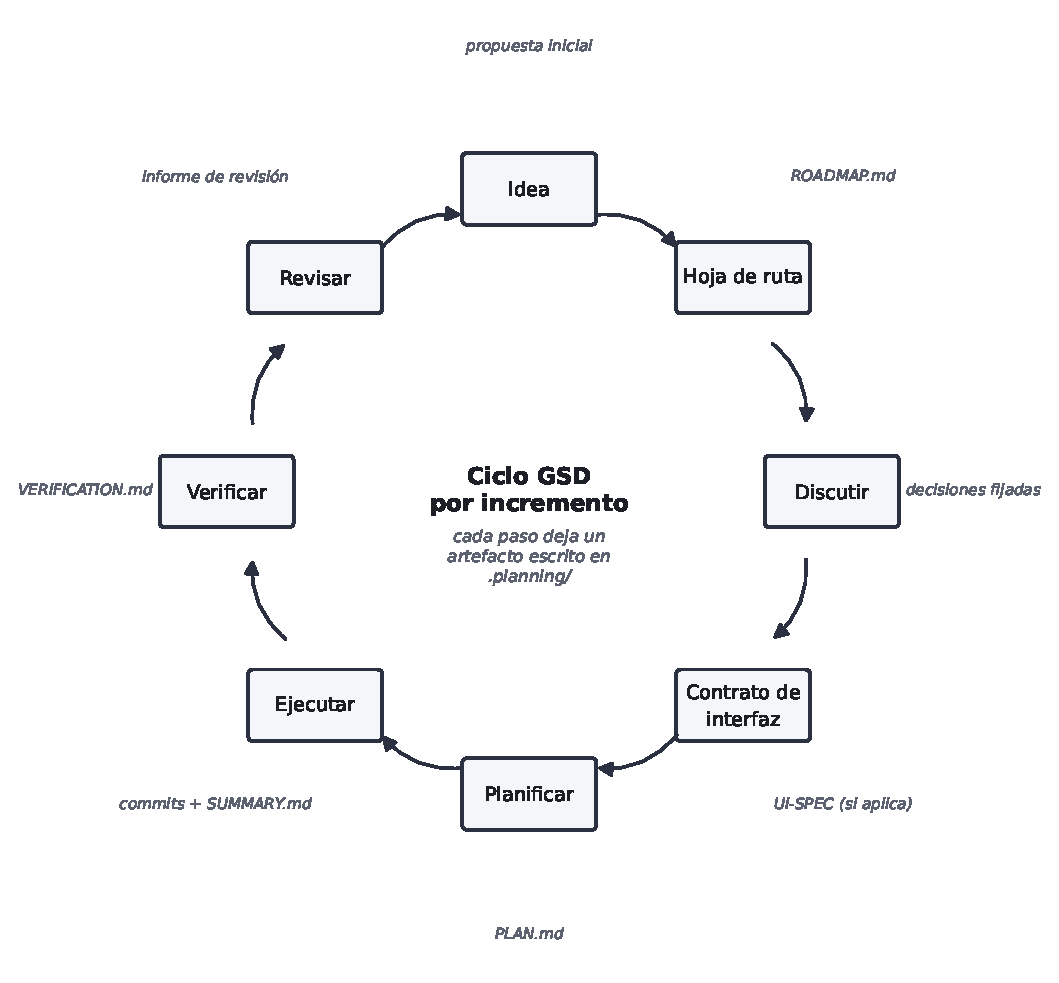
\includegraphics[width=0.90\textwidth]{figures/ciclo-gsd.pdf}
    \caption{Ciclo de un incremento en el método GSD y los artefactos que produce cada paso.}
    \label{fig:ciclo-gsd}
\end{figure}

En la práctica, cada incremento se abre con una discusión que fija por escrito sus decisiones
y supuestos. Si tiene interfaz, se establece además un contrato de diseño con sus componentes
y estados. A continuación se investiga y se redacta el plan, que lo descompone en tareas
atómicas con criterios de aceptación y se comprueba antes de tocar código. La ejecución
implementa ese plan, confirma los cambios en el control de versiones y registra en un resumen
lo realmente hecho y las desviaciones. Por último, la verificación comprueba, de forma
independiente, que el objetivo se ha alcanzado. Una revisión de código somete después los
cambios a un análisis de seguridad, rendimiento y corrección con un contexto distinto del que
los escribió. Cada incremento termina con una firma de aceptación del proyecto. Las órdenes de este flujo
(\texttt{discuss-phase}, \texttt{ui-phase}, \texttt{plan-phase}, \texttt{execute-phase},
\texttt{verify-work} y \texttt{code-review}), junto con \texttt{pause-work} y \texttt{resume-work} para
retomar el trabajo entre sesiones, se usaron de verdad durante el proyecto.

\section{Planificación viva y trazabilidad}\label{sec:met-planning}\label{sec:gestion-gsd}\label{sec:met-trazabilidad}\label{sec:met-incidencias}\label{sec:gestion-obsidian}

La cadena de artefactos que produce cada paso vive en el árbol \texttt{.planning/} del repositorio, que actúa como
la memoria de trabajo compartida entre el autor y los agentes. \texttt{PROJECT.md} recoge el
encuadre general del proyecto y las decisiones de producto que no cambian de un incremento a otro.
\texttt{REQUIREMENTS.md} mantiene el catálogo de requisitos con su identificador, su estado y
el incremento que lo cierra, de forma que un requisito se puede seguir desde que se declara hasta que
queda marcado como completo. \texttt{ROADMAP.md} descompone el proyecto en incrementos con sus planes
y su progreso, numerados en orden y con decimales (como el 01.1) cuando se inserta uno posterior. \texttt{STATE.md} conserva un resumen del punto en el que se encuentra el
trabajo, con referencia al último commit relevante, pensado para que una sesión nueva, humana o
de agente, pueda retomar el hilo sin releer todo el historial. Cada incremento añade además, dentro de
\texttt{.planning/phases/}, un par de documentos por plan: un \texttt{PLAN.md} que describe qué
se va a hacer y cómo se va a verificar y un \texttt{SUMMARY.md} que el agente ejecutor redacta
al terminar, con lo que se hizo, las desviaciones respecto al plan original y la evidencia que
lo respalda. Esta cadena de documentos es la que permite responder, meses después, a la
pregunta de por qué existe una línea de código concreta: se remonta al plan que la motivó, a la
verificación que la aceptó y al requisito que la justificaba, sin depender de la memoria de
nadie.

La Tabla~\ref{tab:planning-arbol} enumera los artefactos principales del árbol y su función.

\begin{table}[H]
\centering
\begin{tabularx}{\textwidth}{ | L{0.44\textwidth} | Y | }
    \hline
    \textbf{Artefacto} & \textbf{Función} \\
    \hline
    \texttt{PROJECT.md} & Definición del producto, valor central, requisitos activos y fuera de alcance. \\
    \hline
    \texttt{REQUIREMENTS.md} & Catálogo de requisitos con identificador estable y matriz de trazabilidad a evidencia. \\
    \hline
    \texttt{ROADMAP.md} & Incrementos, objetivos, criterios de éxito y progreso. \\
    \hline
    \texttt{STATE.md} & Estado actual, posición, decisiones acumuladas y continuidad de sesión. \\
    \hline
    \path{phases/<incremento>/<plan>-PLAN.md} & Alcance y criterios de aceptación de un plan, antes de implementar. \\
    \hline
    \path{phases/<incremento>/<plan>-SUMMARY.md} & Lo realmente ejecutado, desviaciones y evidencias, al cerrar el plan. \\
    \hline
    \path{phases/<incremento>/<incremento>-VERIFICATION.md} & Verificación independiente del objetivo del incremento. \\
    \hline
    \path{phases/<incremento>/deferred-items.md} & Hallazgos fuera de alcance, enrutados a trabajo posterior. \\
    \hline
\end{tabularx}
\caption{Artefactos principales del árbol \texttt{.planning/}.}
\label{tab:planning-arbol}
\end{table}

La trazabilidad se apoya en tres mecanismos. El primero es la matriz de
\texttt{REQUIREMENTS.md}, que registra el estado de cada requisito y la evidencia que lo
cierra, de modo que cualquier requisito se puede seguir hasta el trabajo que lo entrega y
hasta la prueba que lo respalda. El segundo es la correspondencia entre planes e incidencias:
cada plan tiene una incidencia (\textit{issue}) abierta en el repositorio, que los mensajes de
commit referencian con \texttt{Refs \#N} mientras el plan avanza y que se cierra con
\texttt{Closes \#N} cuando el \texttt{SUMMARY.md} confirma que quedó ejecutado, integrado y
verificado. Así el historial de incidencias muestra, sin abrir el árbol \texttt{.planning/}, qué
trabajo está cerrado y con qué evidencia. El tercero es el registro
de agentes descrito en la Sección~\ref{sec:met-ledger}, que ata cada artefacto a la acción
que lo produjo mediante un hash de contenido. Entre los tres, una decisión de la memoria se
puede recorrer hacia atrás hasta su plan, su requisito y su discusión; hacia delante llega
hasta la prueba y la firma que la verifican.

Además del registro de agentes, el proyecto conserva dos registros de decisión. Los ítems
diferidos, en \texttt{deferred-items.md}, recogen los hallazgos fuera de alcance descubiertos
durante la ejecución, con su motivo y su destino. Los registros de decisión de arquitectura (ADR),
en \texttt{docs/adr/}, documentan cada decisión material con su contexto, sus alternativas,
su decisión, su evidencia, sus consecuencias y su reversibilidad. El
Capítulo~\ref{cap:diseno} resume los nueve registros de decisión de arquitectura vigentes.

El árbol \texttt{.planning/} es la fuente de verdad operativa, pero no está pensado para
explorar cómo se relacionan las ideas entre sí. Para eso, el proyecto mantiene además un
\textit{vault} de Obsidian, \texttt{ideas-vault/}, una colección de notas en Markdown
enlazadas entre sí mediante referencias internas que Obsidian representa como un grafo
navegable. Cada nota recoge un concepto (una decisión de diseño, un requisito, un algoritmo,
un incremento); sus enlaces señalan de qué otras notas depende o a cuáles afecta, de modo que
retomar un concepto después de semanas sin tocarlo no exige reconstruir el contexto desde
cero: basta con abrir su nota y seguir sus enlaces. La Figura~\ref{fig:obsidian-vault} muestra
el grafo real del vault de SavePoint en el momento de escribir esta memoria, generado a partir
de los enlaces existentes entre sus notas, no como una ilustración esquemática.

\begin{figure}[H]
    \centering
    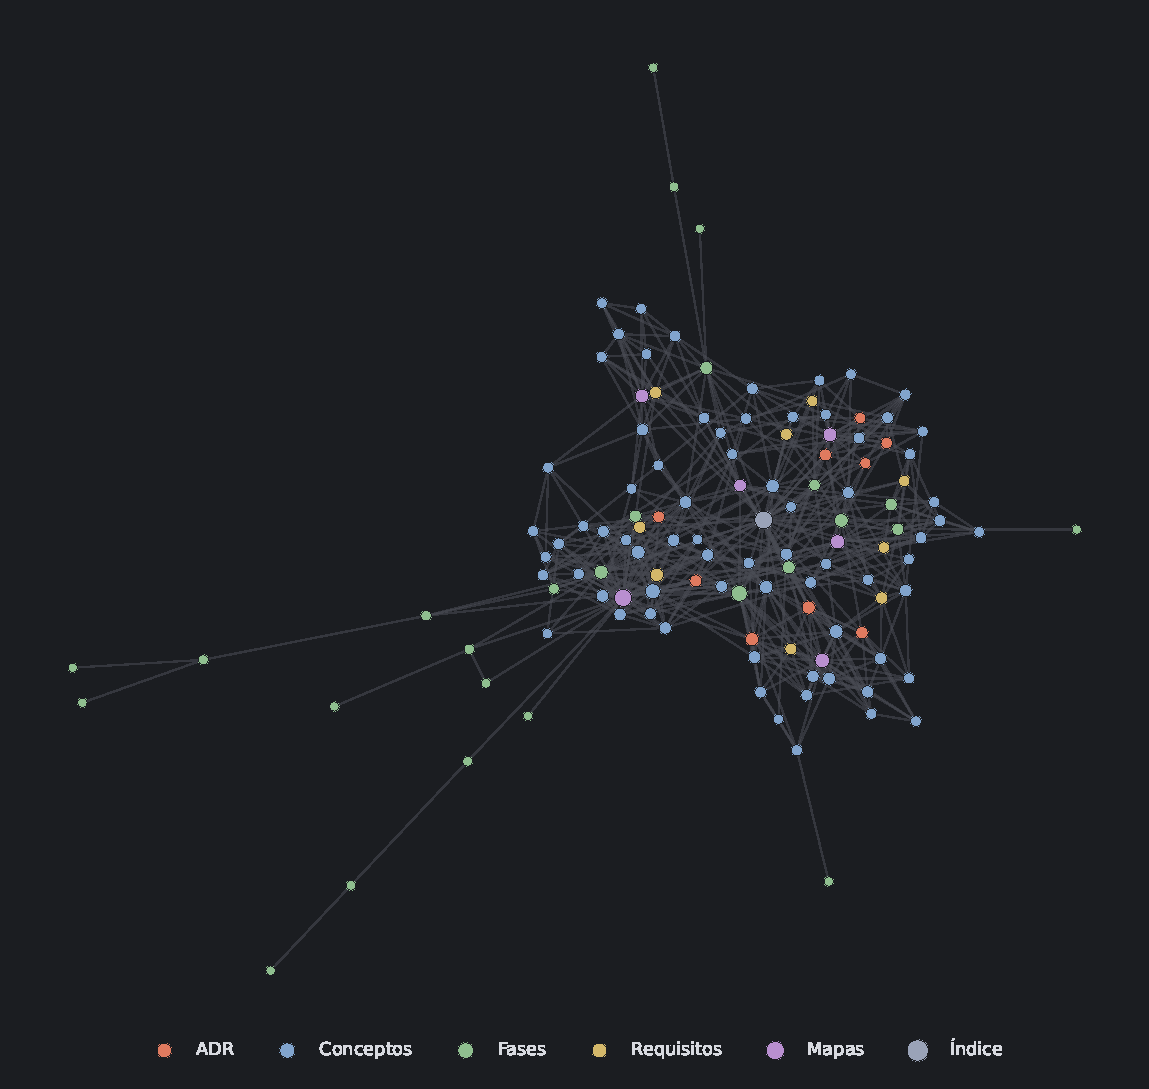
\includegraphics[width=0.92\textwidth]{figures/obsidian-vault-graph.pdf}
    \caption[Grafo del vault de Obsidian de SavePoint]{Grafo del vault de Obsidian de SavePoint (\texttt{ideas-vault/}), coloreado por
    categoría de nota. Se muestra la componente conexa principal, ciento veintitrés notas de
    las ciento cincuenta que contiene el vault; el resto enlaza solo entre sí en subgrafos
    pequeños y aislados. Los nodos de mayor tamaño, como \texttt{00 - Indice} o los mapas de
    investigación y de datos, son las notas con más enlaces entrantes y salientes.}
    \label{fig:obsidian-vault}
\end{figure}

El vault y el árbol \texttt{.planning/} cumplen papeles distintos y deliberadamente no
redundantes. El árbol de planificación es normativo: fija alcance, criterios de aceptación y
evidencia; de él depende que un plan se dé o no por cerrado. El vault es descriptivo: enlaza
conceptos con las fuentes canónicas que los sustentan (un ADR, un requisito, un incremento) para que
se puedan explorar sus relaciones de forma visual, pero nunca sustituye a las pruebas, a los
hashes ni a los artefactos versionados que certifican una decisión. Esta separación se aplicó
también a la propia redacción de esta memoria: antes de escribir varios de los capítulos que
siguen, resultó más rápido navegar el grafo del vault para recuperar cómo encajaban entre sí
conceptos ya explorados en sesiones distintas, semanas atrás, que releer el historial completo
de decisiones desde cero.

\section{Agentes especializados y contrato de contexto}\label{sec:met-agentes}\label{sec:met-subagentes}\label{sec:gestion-subagentes}\label{sec:gestion-worktrees}\label{sec:gestion-skills}\label{sec:met-contrato-contexto}\label{sec:gestion-contrato}\label{sec:gestion-memoria}\label{sec:met-ledger}\label{sec:gestion-ledger}\label{sec:met-convenciones}

El proyecto se desarrolló con asistencia sistemática de los agentes especializados que define
GSD. Conviene delimitar desde el principio el reparto de responsabilidades, que la
Sección~\ref{sec:met-encuadre} retoma: los agentes ejecutan, mientras que la definición del
alcance, los criterios de aceptación, la revisión de cada entrega y la decisión final son
del proyecto. El uso de agentes se describe aquí como una metodología de trabajo que se
diseñó, dirigió y evaluó, no como una coautoría.

El método de la Sección~\ref{sec:arte-agentes} se instrumenta en SavePoint con tres mecanismos.
El primero es ese aislamiento del contexto: cada tarea atómica la ejecuta una instancia nueva del
agente y la información viaja por los ficheros persistentes del árbol \texttt{.planning/}
(Sección~\ref{sec:met-planning}), de modo que una interrupción, un límite de sesión o un
cambio de día no hacen perder el hilo. El segundo es la especialización de esas instancias en
los papeles de la Tabla~\ref{tab:subagentes}: quien planifica, quien implementa y quien
verifica son instancias independientes, de modo que la verificación no hereda la confianza
del código recién escrito, igual que en un equipo humano se separan el desarrollo y la
revisión.

\begin{table}[H]
\centering
\begin{tabularx}{\textwidth}{ | L{0.34\textwidth} | Y | }
    \hline
    \textbf{Rol} & \textbf{Responsabilidad y límite} \\
    \hline
    \texttt{gsd-phase-researcher} & Recopila y sintetiza evidencia para planificar un incremento. Propone; etiqueta fuente, evidencia o supuesto. \\
    \hline
    \texttt{gsd-ui-researcher} / \texttt{gsd-ui-checker} & Convierten los requisitos en un contrato de diseño y lo validan. La comprobación automática de accesibilidad no sustituye la revisión humana. \\
    \hline
    \texttt{gsd-planner} & Divide el alcance en tareas verificables. Propone secuencia y gates; no declara terminado el producto. \\
    \hline
    \texttt{gsd-executor} & Implementa, prueba y registra correcciones en una copia de trabajo aislada, con commits atómicos. No se presenta como verificación independiente. \\
    \hline
    \texttt{gsd-verifier} & Verifica el objetivo del incremento de forma independiente y escribe el informe de verificación. \\
    \hline
    \texttt{gsd-code-reviewer} & Revisa todo el repositorio en busca de defectos con un contexto propio, distinto del de la implementación. \\
    \hline
\end{tabularx}
\caption{Subagentes empleados y su responsabilidad.}
\label{tab:subagentes}
\end{table}

El tercer mecanismo traslada ese aislamiento al sistema de ficheros mediante \textit{worktrees} de Git, copias de trabajo independientes que
comparten el mismo historial de repositorio pero permiten que varios agentes ejecutores avancen
en paralelo sin pisarse los cambios. El ciclo de un ejecutor es siempre el mismo: se crea un
\textit{worktree} nuevo para el plan que le corresponde, el agente trabaja y hace sus
\textit{commits} dentro de esa copia aislada, al terminar se integra el resultado en la rama
principal mediante una fusión sin avance rápido (\texttt{merge --no-ff}), que conserva visible
en el historial el conjunto de cambios de ese plan como una unidad; por último, se limpia el
\textit{worktree}. Cuando varios planes de un mismo incremento declaran el mismo requisito, la
orquestación añade además una comprobación de que todos esos planes tienen ya su
\texttt{SUMMARY.md} antes de marcar el requisito como cerrado, para que ningún requisito quede
completo mientras una de sus partes sigue pendiente en otro plan.

Además de los subagentes, el repositorio versiona \textit{skills}: procedimientos empaquetados
que un agente puede invocar para una tarea concreta y repetible, como revisar código con un
criterio fijo o preparar una entrega. Al vivir dentro del repositorio, junto al código que
producen, las \textit{skills} quedan sujetas al mismo control de versiones, a la misma revisión
y al mismo historial que cualquier otro artefacto del proyecto. El entorno de trabajo del
agente deja así de ser una configuración personal invisible para convertirse en parte del
entregable: cualquiera que clone el repositorio dispone del mismo procedimiento que se empleó
durante el desarrollo, no solo del resultado final.

Todo agente que empieza a trabajar en el repositorio, sea la herramienta que sea, lee primero
un conjunto fijo de ficheros de instrucciones que actúan como su contrato de contexto:
\texttt{AGENTS.md}, \texttt{CLAUDE.md} y \texttt{.github/copilot-instructions.md} declaran las
reglas que cualquier asistente debe seguir en este proyecto, mientras que
\texttt{CONVENTIONS.md} fija las convenciones concretas de idioma, de nomenclatura y de flujo de
trabajo con incidencias. Un ejemplo transversal de regla en ese contrato es la convención de
idioma del proyecto: la documentación de este TFG se escribe en español, el código y sus
comentarios se escriben en inglés. Esa regla se aplica sin excepción con independencia de qué
herramienta esté trabajando en cada momento, precisamente porque vive en un fichero que todas
ellas leen al empezar, en lugar de depender de que alguien la recuerde y la repita en cada
conversación.

Sobre ese mismo contrato se apoyan los ficheros de memoria del agente, que sobreviven entre
sesiones: cuando un error del agente o una corrección del proyecto tiene valor general, se
destila en una regla que se relee al iniciar cada tarea, de modo que el fallo no se repite. El
proyecto acumuló varias reglas de este tipo a partir de incidencias reales:

\begin{itemize}
    \item La lista de identificadores de Wikidata escrita a mano en el guion de adquisición
    contenía entidades que no eran videojuegos. La regla derivada obliga a verificar en vivo
    cualquier identificador de Wikidata antes de usarlo, sin confiar en la memoria ni en un
    commit anterior.
    \item El primer intento de cargar el catálogo de IGDB junto al corpus de Wikidata abortó
    por una colisión de \textit{slug} de plataforma. La corrección enseñó al importador a
    reconciliar una plataforma existente por \textit{slug}, nombre e inserción dentro de un
    savepoint, en lugar de fallar.
    \item Los enganches de GSD fallaban en Windows por un problema de shell. Detectarlo y
    corregirlo pronto evitó que el resto del trabajo tropezara con lo mismo.
    \item Sin un montaje enlazado de Docker y sin cargar el módulo de configuración de Django
    dentro del contenedor, toda verificación posterior habría probado una imagen obsoleta o
    habría fallado al arrancar. Corregir ambos al detectarlos evitó que el trabajo siguiente
    chocara con la misma pared.
\end{itemize}

El componente más distintivo del proceso es el registro de agentes,
\texttt{docs/methodology/agent-ledger.jsonl}, un fichero de solo anexado con un objeto por
línea. Cada entrada lleva una marca de tiempo, un tipo, el actor, el objetivo, las entradas y
salidas referenciadas por ruta relativa y hash SHA-256 (del inglés \textit{secure hash algorithm}), las herramientas empleadas sin sus
secretos, el resultado y las limitaciones declaradas. El tipo es uno de tres:
\texttt{proposal} para una propuesta de agente, \texttt{automated-check} para una
comprobación determinista y \texttt{author-decision} para una decisión humana, que siempre
identifica al actor como persona. El registro contiene veinticinco entradas. El gate
\texttt{scripts/check-evidence.ps1} valida su esquema, sus tipos, sus actores, sus rutas, sus
hashes y su cobertura, probando primero con entradas inválidas antes de dar por buena una
ejecución limpia.

El registro es una convención auditable, no un almacén criptográficamente inmutable: Git
conserva las revisiones y el gate detecta corrupción de referencias en el estado actual, pero
un actor con permiso de escritura podría reescribir el historial. Para la evidencia final se
firma o etiqueta el commit correspondiente. El registro es honesto sobre sus propios huecos:
donde un artefacto histórico resultó irrecuperable, la entrada lo declara en sus campos de
entradas no verificables y de limitaciones en lugar de ocultarlo o falsearlo. También registra
que el proyecto usó más de un entorno de agente, con modelos distintos en el
trabajo inicial y en el posterior, con la advertencia de que un nombre de
modelo no basta para reproducir una salida probabilística: la evidencia reproducible son los
artefactos versionados, los hashes, los comandos y las decisiones humanas.
Los mensajes de commit siguen el estilo de \textit{Conventional Commits} y se escriben en
inglés.

\section{Planificación del laboratorio de evaluación}\label{sec:met-fase2}

El laboratorio de evaluación se planificó como el puente entre la demostración de producto y la evaluación
reproducible. Su objetivo no era añadir una pantalla aislada, sino fijar las condiciones que
permiten afirmar algo sobre un recomendador: qué obras entran en el corpus, qué significan
las valoraciones, qué usuarios se simulan, cómo se construyen los candidatos y con qué
métricas se comparan las listas. Las decisiones metodológicas se tomaron antes de cualquier
ejecución de laboratorio y se conservaron en el directorio de planes del incremento.

El orden no es accidental. El corpus y la versión inmutable preceden al protocolo; el protocolo
precede a la generación de usuarios y a la implementación de variantes; y solo entonces se
puede ejecutar una comparación con garantías de que todos los algoritmos han recibido la
misma partición y el mismo conjunto de candidatos. Una tarea completada ha superado las
verificaciones de su contrato, pero no demuestra una superioridad algorítmica.

Las decisiones que bloquean una comparación posterior quedaron congeladas en
\texttt{docs/methodology/protocol.json} y en \texttt{docs/methodology/evaluation-protocol.md}:
el corpus, el significado de las valoraciones, la población sintética, la relevancia, el
conjunto de candidatas y las métricas. Esta sección solo recoge cómo se planificó esa
congelación; el contenido de cada decisión se describe donde se aplica. El corpus y las
valoraciones, en la Sección~\ref{cap:datos}; el diseño del laboratorio, en la
Sección~\ref{sec:dis-laboratorio}; y el protocolo con el que se publicaron los resultados, en
la Sección~\ref{sec:exp-protocolo}.

\section{Planificación temporal}\label{sec:met-temporal}

El trabajo se planificó como una sucesión de incrementos verticales, cada uno utilizable y
verificado antes de abordar el siguiente, en lugar de un calendario cerrado de tareas fijado
desde el principio. El desarrollo se organizó en seis iteraciones a lo largo de dos meses,
desde principios de agosto hasta el 4 de octubre de 2026, agrupadas alrededor de los hitos de la
Tabla~\ref{tab:hitos}. El estudio previo y las primeras pruebas de desarrollo comenzaron
aproximadamente un mes antes del arranque sistemático del repositorio de producto: el
repositorio se creó el 24 de agosto y el desarrollo con registros de decisión y planes por
incremento comenzó el 4 de septiembre. La fecha de inicio del estudio previo es aproximada; las
posteriores proceden del historial del repositorio y de las firmas de cada incremento.

\begin{table}[H]
\centering
\caption{Lista de hitos del trabajo.}\label{tab:hitos}
\begin{tabularx}{\textwidth}{ | Y | C{0.20\textwidth} | }
    \hline
    \textbf{Hito} & \textbf{Fecha} \\
    \hline
    H0: Inicio del estudio previo y de las primeras pruebas de desarrollo & 04/08/2026 \\
    \hline
    H1: Demostración pública de tres días en producción & 05/09/2026 \\
    \hline
    H2: Catálogo a escala real e interfaz rediseñada & 06/09/2026 \\
    \hline
    H3: Contrato de evaluación sin conexión congelado & 08/09/2026 \\
    \hline
    H4: Recomendadores de contenido, colaborativo e híbrido implementados & 12/09/2026 \\
    \hline
    H5: Publicación de resultados v15 con significación estadística & 12/09/2026 \\
    \hline
    H6: Flujos de colección, relaciones de amistad y endurecimiento cerrados & 14/09/2026 \\
    \hline
    H7 — Memoria del TFG y despliegue completos, listos para defensa & 04/10/2026 \\
    \hline
\end{tabularx}
\end{table}

La Figura~\ref{fig:calendario} sitúa las iteraciones y los hitos en el calendario.

\begin{figure}[htp]
    \centering
    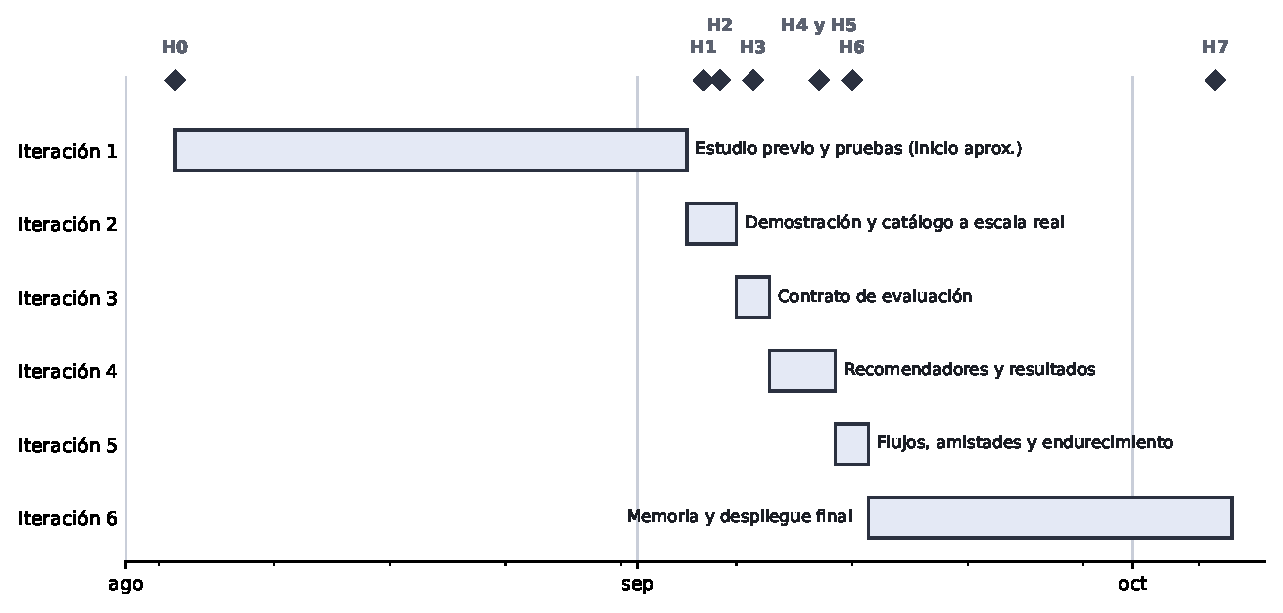
\includegraphics[width=0.9\textwidth]{figures/calendario-iteraciones.pdf}
    \caption{Calendario de las iteraciones y de los hitos H0 a H7 del trabajo.}
    \label{fig:calendario}
\end{figure}

La \textbf{Iteración 1} (de principios de agosto al 3 de septiembre, con inicio aproximado) cubrió el
estudio previo y las primeras pruebas de desarrollo: revisión de productos de referencia,
comparación de fuentes de datos de videojuegos y sus licencias y pruebas de desarrollo
previas al arranque del repositorio de producto. La \textbf{Iteración 2} (4 al 6 de septiembre)
formalizó las primeras decisiones de arquitectura (ADR-001 y ADR-002) con un entorno de
desarrollo reproducible en Docker Compose y entregó el primer incremento de producto bajo una
restricción explícita de tres días para una demostración pública visible, con un catálogo
reducido, una cuenta y la recomendación por popularidad; a continuación amplió el catálogo a
escala real e incorporó el rediseño de la interfaz. La \textbf{Iteración 3} (7 y 8 de
septiembre) congeló el contrato de evaluación sin conexión: corpus, población sintética, métricas y
protocolo, antes de escribir ningún algoritmo de recomendación avanzado. La
\textbf{Iteración 4} (9 al 12 de septiembre) implementó las tres familias de recomendación
(contenido, colaborativo e híbrido) y sus dieciséis variantes y ejecutó la publicación final de
resultados (v15) descrita en el Capítulo~\ref{cap:resultados}. La \textbf{Iteración 5} (13 y 14
de septiembre) cerró los flujos completos de colección y portabilidad, las relaciones de
amistad y el endurecimiento de seguridad. La \textbf{Iteración 6} (15 de septiembre al 4 de
octubre) se dedicó a la redacción, revisión y cierre de esta memoria y del despliegue, junto con
los ajustes finales de la interfaz y del módulo social.

\section{Estimación de esfuerzo y presupuesto}\label{sec:met-presupuesto}

El proyecto no llevó un registro de horas minuto a minuto por tarea, de modo que la estimación
de esfuerzo que sigue se reconstruye a partir de la duración de cada iteración y de la carga de
trabajo declarada de un estudiante que compagina el TFG con otras obligaciones académicas,
en torno a treinta y cuatro horas semanales durante las nueve semanas transcurridas desde el inicio
del estudio previo hasta el cierre de la memoria, unas trescientas diez horas en total. Tomando
como unidad el bloque de trabajo, no el incremento, la Tabla~\ref{tab:presupuesto-horas}
reparte esas horas entre las grandes áreas del trabajo.

\begin{table}[H]
\centering
\caption{Estimación de horas por bloque de trabajo.}\label{tab:presupuesto-horas}
\begin{tabularx}{\textwidth}{ | Y | C{0.20\textwidth} | }
    \hline
    \textbf{Bloque} & \textbf{Horas estimadas} \\
    \hline
    Análisis, requisitos y diseño & 41 \\
    \hline
    Infraestructura reproducible y despliegue & 25 \\
    \hline
    Implementación de producto (backend y frontend) & 86 \\
    \hline
    Adquisición y gobierno de datos & 28 \\
    \hline
    Algoritmos de recomendación y protocolo de evaluación & 63 \\
    \hline
    Pruebas, verificación y revisión & 31 \\
    \hline
    Redacción de la memoria & 36 \\
    \hline
    \textbf{Total} & \textbf{310} \\
    \hline
\end{tabularx}
\end{table}

El coste directo se calcula sobre esas 310 horas con una tarifa de referencia de un perfil
junior de ingeniería del software en España, 14,00\,€/hora, una cota conservadora frente al
coste real de contratación de un perfil equivalente. El coste material recoge la amortización
proporcional del ordenador de torre empleado, valorado en 1.000,00\,€ y con una vida útil estimada de
cuatro años, del que este trabajo consume dos meses. Se añade una suscripción a agentes de IA,
estimada en 30,00\,€, empleada como apoyo al desarrollo bajo dirección y revisión humanas. No
se incluye ningún coste de infraestructura en la nube, porque la topología de despliegue público
se diseñó explícitamente de coste cero (ADR-005, Sección~\ref{cap:despliegue}). El coste
indirecto recoge la cuota proporcional de dos meses de electricidad y conexión a internet
atribuible al proyecto. La Tabla~\ref{tab:presupuesto} resume el presupuesto total.

\begin{table}[H]
\centering
\begin{tabularx}{\textwidth}{ | Y | C{0.22\textwidth} | }
    \hline
    \textbf{Concepto} & \textbf{Coste (\euro{})} \\
    \hline
    Coste directo (310\,h a 14,00\,€/h) & 4.340,00 \\
    \hline
    Coste material (amortización de ordenador de torre, 2 meses) & 41,67 \\
    \hline
    Suscripción a agentes de IA & 30,00 \\
    \hline
    Costes indirectos (electricidad y conexión, 2 meses) & 90,00 \\
    \hline
    \textbf{Presupuesto total} & \textbf{4.501,67} \\
    \hline
\end{tabularx}
\caption{Estimación de esfuerzo y presupuesto del proyecto.}
\label{tab:presupuesto}
\end{table}

Estas cifras son una estimación reconstruida a posteriori, no una medición registrada durante
el desarrollo; así debe entenderse cualquier comparación futura entre coste estimado y coste
real.

\section{Riesgos y mitigaciones}\label{sec:met-riesgos}

La Tabla~\ref{tab:riesgos} recoge los riesgos identificados, su probabilidad e impacto
cualitativos y la mitigación aplicada o prevista. La escala empleada es baja, media y alta;
la valoración expresa la exposición del proyecto en el momento de planificar cada medida.

\begin{table}[H]
\centering
\begin{tabularx}{\textwidth}{ | L{0.23\textwidth} | C{0.17\textwidth} | C{0.12\textwidth} | Y | }
    \hline
    \textbf{Riesgo} & \textbf{Probabilidad} & \textbf{Impacto} & \textbf{Mitigación} \\
    \hline
    Restricción de tres días del primer incremento público & Alta & Alta & Alcance de demostración deliberadamente estrecho: catálogo pequeño, una cuenta y recomendación por popularidad. \\
    \hline
    Términos legales de las fuentes de datos & Media & Alta & Confirmación caso por caso: corpus de Wikidata bajo dominio público, términos de IGDB registrados textualmente y reconciliados en un registro de decisión. \\
    \hline
    Volumen de IGDB en una importación larga & Media & Media & Importador reanudable por cursor de identificador, con checkpoint tras cada lote y resistencia probada a una interrupción. \\
    \hline
    Portadas por enlace directo a un tercero & Media & Media & Ventana de retención de treinta días asumida; ausencia o fallo de una portada cae a un marcador propio. \\
    \hline
    El protocolo de evaluación debe congelarse antes de comparar recomendadores & Media & Alta & El heurístico de géneros del sistema se declaró explícitamente fuera de esa comparación desde el principio; la comparación en sí se congeló y se ejecutó más tarde, como recoge el Capítulo~\ref{cap:resultados}. \\
    \hline
    Errores del agente en trabajo dado por bueno & Media & Alta & Verificación de objetivos independiente y revisión de código de todo el repositorio con contexto propio. \\
    \hline
    Catálogo parcial en el despliegue público & Alta & Media & El corpus gobernado completo no cabe en el nivel gratuito de la base de datos; se publica un subconjunto con criterio explícito y el entorno local reproducible es donde se mide la evaluación (Sección~\ref{cap:despliegue}). \\
    \hline
\end{tabularx}
\caption{Riesgos identificados y sus mitigaciones.}
\label{tab:riesgos}
\end{table}

\section{Lecciones aprendidas y valoración de la metodología}\label{sec:met-desviaciones}\label{sec:met-encuadre}\label{sec:gestion-beneficios}\label{sec:gestion-limitaciones}

El trabajo dejó varias lecciones de ingeniería que conviene recoger. La primera tiene que ver
con el despliegue. La topología pasó de un único proveedor con
predespliegue para las dos imágenes de contenedor a tres servicios gratuitos coordinados, al
chocar la restricción de coste cero con el modelo de un solo proveedor. La decisión y sus
consecuencias quedaron documentadas en un registro de decisión de arquitectura, de modo que
la diferencia entre el despliegue público y el entorno local es una elección deliberada y
no una divergencia de comportamiento.

La segunda es de higiene del propio proceso: un gate de evidencia llegó a estar en rojo en la
rama principal por un problema de fin de línea y por registros de decisión escritos en inglés
antes de fijarse la convención de idioma. Corregirlo en cuanto se detectó evitó que el resto
del trabajo arrastrara un gate poco fiable. Estas incidencias, junto con otras menores,
quedaron registradas en los resúmenes de plan.

El enfoque produjo beneficios concretos y observables en el proyecto, junto con límites que
conviene declarar con la misma franqueza. El alcance se mantuvo bajo control a lo largo de
sucesivos incrementos, sin que el trabajo de uno se filtrara en otro y cada cambio quedó
trazado hasta su plan, su requisito y su evidencia. Las revisiones de código con contexto
independiente encontraron dieciséis hallazgos reales, descritos en la
Sección~\ref{cap:pruebas}, que se corrigieron por completo, incluidos defectos de seguridad en
trabajo ya dado por bueno. El trabajo se pudo reanudar sin pérdida de hilo tras interrupciones
y límites de sesión, porque el estado vivía en ficheros y no en una conversación y el propio
proceso de ingeniería quedó reproducible, no solo el producto: un tercero puede clonar el
repositorio y reconstruir la historia de decisiones a partir del árbol de planificación, los
registros de decisión, el registro de agentes y los gates de evidencia.

El enfoque depende, sin embargo, de la calidad de la especificación escrita: un plan ambiguo
produce una ejecución ambigua. Mantener la disciplina de planificación, verificación y registro
tiene un coste de tiempo notable para un TFG individual; los agentes cometieron errores que
hubo que detectar y corregir, algunos de ellos recogidos en la
Sección~\ref{sec:met-contrato-contexto}. Un agente no es un evaluador independiente de su
propia propuesta, del mismo modo que un hash prueba identidad de bytes, no veracidad ni calidad;
por eso el enfoque no sustituye el juicio del proyecto sobre arquitectura, alcance y aceptación,
sino que lo enmarca. Existe un informe de uso de herramientas de asistencia, independiente y
posterior, que cubre la transparencia de su empleo; esta memoria ni lo suple ni lo contradice.

Los capítulos siguientes aplican ese método al análisis, al diseño y a la construcción del sistema.

    \chapter{Análisis del problema}\label{cap:analisis}\label{cap:requisitos}\label{ap:req-detallados}

Este capítulo recoge el análisis de requisitos del proyecto. Presenta los actores del
sistema, el modelo de dominio que sostiene los requisitos de información, los requisitos
funcionales y no funcionales, las reglas de negocio, los casos de uso y la matriz de
trazabilidad que enlaza cada requisito con su evidencia. Los
requisitos se identifican con códigos estables tomados de \texttt{.planning/REQUIREMENTS.md},
de modo que la matriz de trazabilidad de este capítulo y la del repositorio coinciden. Los
requisitos abarcan por igual las dos caras del trabajo: la plataforma de catalogación y la
evaluación de recomendadores que se apoya en ella.

\section{Actores del sistema}\label{sec:req-actores}

El sistema distingue dos actores, que enumera la Tabla~\ref{tab:actores}. Para que el tribunal
pueda recorrer el sistema sin registrarse, el entorno incluye una cuenta de usuario ya
preparada, que es una cuenta normal con sus datos y no un actor distinto.

\begin{table}[H]
\centering
\begin{tabularx}{\textwidth}{ | L{0.20\textwidth} | Y | }
    \hline
    \textbf{Actor} & \textbf{Descripción} \\
    \hline
    Visitante & Persona no autenticada que consulta el catálogo, la ficha de un juego y la recomendación por popularidad y que puede registrarse. \\
    \hline
    Persona usuaria & Titular de una cuenta registrada que inicia sesión y gestiona su lista de pendientes, valora juegos, inventaría copias y se relaciona con sus amigos. \\
    \hline
\end{tabularx}
\caption{Actores del sistema.}
\label{tab:actores}
\end{table}

\section{Requisitos de información: modelo de dominio}\label{sec:req-informacion}

El modelo de dominio distingue tres áreas: el catálogo, la biblioteca personal y las cuentas.
La Figura~\ref{fig:modelo-dominio} las representa junto con las tablas del laboratorio de
evaluación, que describe la Sección~\ref{sec:dis-laboratorio}; los párrafos siguientes
describen las entidades de las tres primeras. El diagrama de entidades con sus atributos y cardinalidades, tal como lo
implementan los modelos, está en la Sección~\ref{sec:dis-modelo-datos}.

\begin{figure}[H]
    \centering
    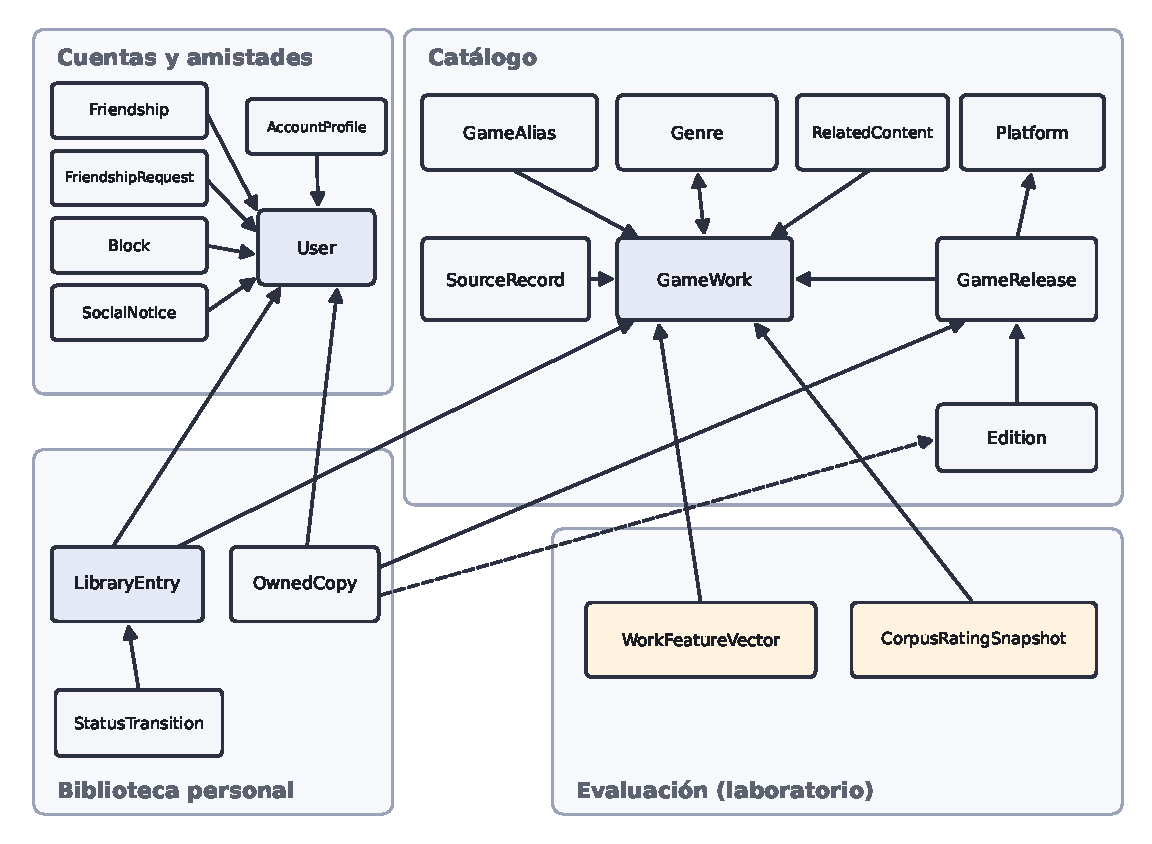
\includegraphics[width=0.95\textwidth]{figures/modelo-dominio.pdf}
    \caption[Modelo de dominio de SavePoint]{Modelo de dominio de SavePoint, agrupado por catálogo, biblioteca personal, cuentas y amistades y laboratorio de evaluación. Cada flecha parte de la entidad que contiene la clave foránea y apunta a la entidad que referencia; la flecha de doble punta indica una relación de muchos a muchos y la discontinua, una referencia opcional. De las copias en propiedad solo se dibujan sus referencias a la versión de lanzamiento y a la edición; \texttt{IgdbImportRun} y \texttt{AssetAttribution} se omiten de la figura y se describen en el texto.}
    \label{fig:modelo-dominio}
\end{figure}

En el catálogo, la entidad central es la obra (\texttt{GameWork}), la identidad canónica de
un título de videojuego con independencia de la plataforma y de la edición. Cada obra puede tener varias publicaciones (\texttt{GameRelease}), una por plataforma
(\texttt{Platform}). Cada publicación puede tener a su vez varias ediciones
(\texttt{Edition}). Los géneros (\texttt{Genre}) se
asocian a la obra mediante una relación de muchos a muchos. Los alias bilingües
(\texttt{GameAlias}) sostienen la búsqueda tolerante. El contenido relacionado (\texttt{RelatedContent}) enlaza
contenido descargable (DLC) y expansiones con su obra padre. La
procedencia de cada obra vive en \texttt{SourceRecord}, con la fuente, el identificador de
origen, la licencia, la fecha de recuperación y un hash del contenido normalizado. La
atribución de cada portada revisada individualmente vive en \texttt{AssetAttribution}, cuya
marca de portada permitida está a falso por defecto. El progreso de una importación de IGDB
se registra en \texttt{IgdbImportRun}, con el cursor de identificador y el estado.

En la biblioteca personal, la entrada de biblioteca (\texttt{LibraryEntry}) representa la
relación entre una persona usuaria y una obra, con su estado en la lista de pendientes y su
valoración. El historial de
transiciones de estado (\texttt{StatusTransition}) es un registro de solo anexado. Las copias
en propiedad (\texttt{OwnedCopy}) representan cada ejemplar, físico o digital, con su formato,
su publicación y su edición.

En las cuentas, el proyecto usa directamente el modelo de usuario de Django
(\texttt{User}), al que se asocian la biblioteca personal y las relaciones de amistad. Las solicitudes (\texttt{FriendshipRequest}), las amistades aceptadas (\texttt{Friendship}) y los bloqueos (\texttt{Block}) son entidades que referencian a dos usuarios. El perfil editable (\texttt{AccountProfile}) guarda el nombre completo, la biografía, la foto, la portada y los ajustes de privacidad y las notificaciones (\texttt{SocialNotice}) avisan de las solicitudes aceptadas y de las recomendaciones añadidas a pendientes.

La Tabla~\ref{tab:req-informacion} enlaza cada área del modelo con los requisitos de
información que satisface.

\begin{table}[H]
\centering
\begin{tabularx}{\textwidth}{ | L{0.16\textwidth} | Y | C{0.16\textwidth} | }
    \hline
    \textbf{Área} & \textbf{Requisito de información} & \textbf{Códigos} \\
    \hline
    Catálogo & Identidad canónica independiente del proveedor de enriquecimiento. & CAT-04 \\
    \hline
    Catálogo & Registro de fuente, licencia, fecha de recuperación y hash por obra. & DATA-02 \\
    \hline
    Catálogo & Metadatos de plataforma, género, edición y fechas de fuentes aprobadas. & CAT-05 \\
    \hline
    Biblioteca & Estado de la lista de pendientes por persona y obra. & LIB-01 \\
    \hline
    Biblioteca & Valoración con escala consistente. & LIB-02 \\
    \hline
    Biblioteca & Copias en propiedad con formato, plataforma y edición. & INV-01, INV-02 \\
    \hline
    Cuentas & Relaciones de amistad y bloqueo entre personas usuarias. & SOCIAL-03 \\
    \hline
\end{tabularx}
\caption{Áreas del modelo de dominio y requisitos de información asociados.}
\label{tab:req-informacion}
\end{table}

\section{Requisitos funcionales y casos de uso}\label{sec:req-funcionales}\label{sec:req-casos-uso}

La Tabla~\ref{tab:req-funcionales} recoge los requisitos funcionales considerados en el
análisis, con su estado real. Los marcados como completos tienen evidencia en las firmas de
aceptación.

\begin{table}[htp]
\centering
\tablecompact
\begin{tabularx}{\textwidth}{ | L{0.15\textwidth} | Y | C{0.14\textwidth} | }
    \hline
    \textbf{Código} & \textbf{Requisito funcional} & \textbf{Estado} \\
    \hline
    AUTH-01 & Iniciar y cerrar sesión en una cuenta controlada. & Completo \\
    \hline
    PROF-01 & Editar el perfil (nombre, foto, portada, favoritos) y su visibilidad. & Completo \\
    \hline
    SOCIAL-03 & Buscar a otra persona por su alias exacto y gestionar solicitudes de amistad, amistades y bloqueos. & Completo \\
    \hline
    SOCIAL-04 & Consultar la colección, las listas y los comentarios de un amigo aceptado; quien no es amigo solo ve el nombre de usuario. & Completo \\
    \hline
    SOCIAL-05 & Recomendar juegos a un amigo y responder a las recibidas. & Completo \\
    \hline
    CAT-01 & Buscar videojuegos por título. & Completo \\
    \hline
    CAT-02 & Filtrar y ordenar el catálogo por metadatos disponibles. & Completo \\
    \hline
    CAT-03 & Ficha de detalle de cada juego con sus datos y su procedencia. & Completo \\
    \hline
    CAT-04 & Identificadores canónicos que no dependen de la API de enriquecimiento. & Completo \\
    \hline
    CAT-06 & Catálogo usable con datos locales si la API no está disponible. & Completo \\
    \hline
    LIB-01 & Marcar un juego como pendiente, jugando, completado o abandonado. & Completo \\
    \hline
    LIB-02 & Valorar un juego con una escala consistente. & Completo \\
    \hline
    LIB-03 & Comentar un juego, con el comentario visible solo para los amigos. & Completo \\
    \hline
    INV-01 & Registrar varias copias de la misma obra. & Completo \\
    \hline
    INV-02 & Registrar formato, plataforma y edición de cada copia. & Completo \\
    \hline
    INV-05 & Las notas privadas y los detalles de compra nunca aparecen en las proyecciones que ven los amigos. & Completo \\
    \hline
    DATA-01 & Conjunto de datos estable, citable y legalmente adecuado. & Completo \\
    \hline
    DATA-02 & El conjunto registra versión, licencia, dirección web (URL) de origen, fecha y hash. & Completo \\
    \hline
    DATA-04 & API de enriquecimiento elegida mediante comparación documentada. & Completo \\
    \hline
    REC-02 & Recomendación de referencia por popularidad. & Completo \\
    \hline
    REC-10 & Página de recomendaciones por géneros según la actividad propia. & Completo \\
    \hline
    REC-03 a REC-09 & Recomendadores basados en contenido, colaborativos e híbridos, con explicaciones y arranque en frío. & Completo \\
    \hline
    PORT-01 a PORT-04 & Exportación e importación de colección, valoraciones y listas. & Completo \\
    \hline
\end{tabularx}
\caption{Requisitos funcionales considerados en el análisis del sistema.}
\label{tab:req-funcionales}
\end{table}

La Figura~\ref{fig:casos-uso} presenta el diagrama de casos de uso del sistema tal como se
analizó al inicio del proyecto. Las funciones incorporadas después, como las listas, los favoritos, la
importación y exportación de la colección y las tres variantes de recomendación publicadas, no añaden actores y
amplían los casos de uso aquí descritos.

\begin{figure}[htp]
    \centering
    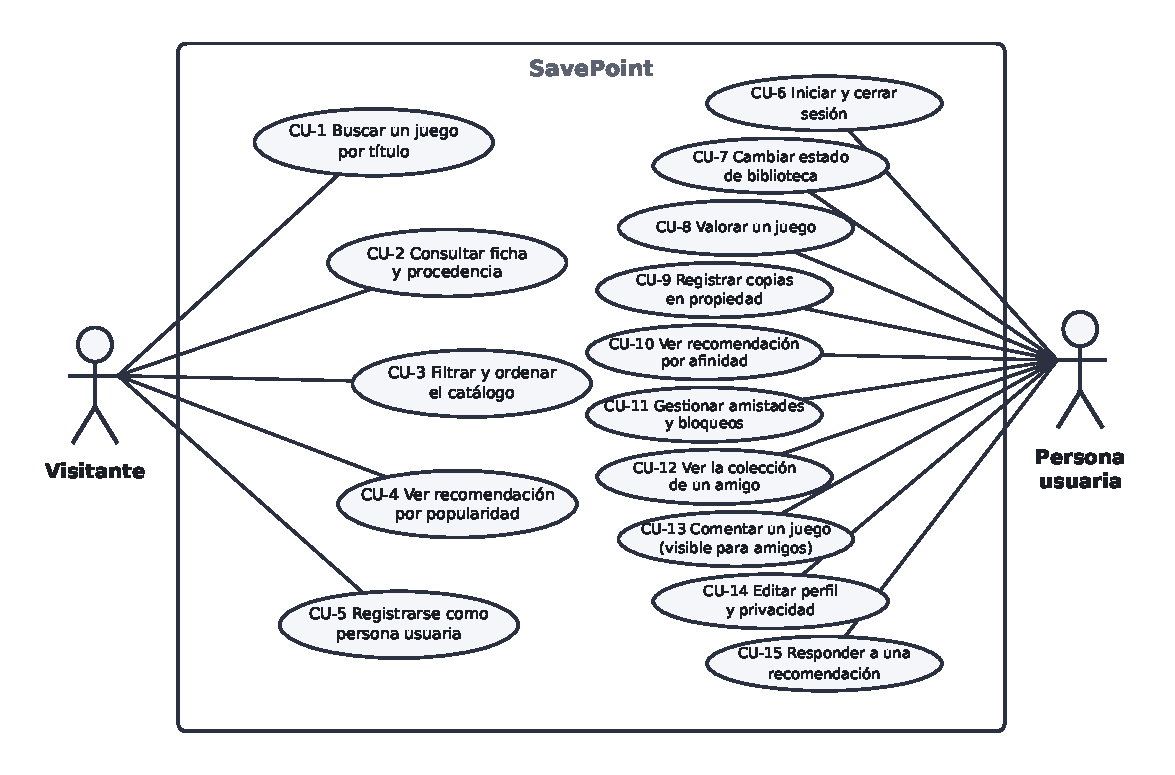
\includegraphics[width=0.95\textwidth]{figures/casos-uso.pdf}
    \caption{Diagrama de casos de uso del sistema, por actor principal. Cada línea une un actor con los casos de uso que ejecuta.}
    \label{fig:casos-uso}
\end{figure}

La Tabla~\ref{tab:casos-uso} describe cada caso de uso con su actor principal y el requisito
funcional que satisface.

\begin{table}[htp]
\centering
\begin{tabularx}{\textwidth}{ | C{0.10\textwidth} | Y | L{0.22\textwidth} | C{0.18\textwidth} | }
    \hline
    \textbf{Id} & \textbf{Caso de uso} & \textbf{Actor} & \textbf{Requisito} \\
    \hline
    CU-1 & Buscar un juego por título & Visitante & CAT-01 \\
    \hline
    CU-2 & Consultar la ficha de un juego y su procedencia & Visitante & CAT-03 \\
    \hline
    CU-3 & Filtrar y ordenar el catálogo & Visitante & CAT-02 \\
    \hline
    CU-4 & Ver la recomendación por popularidad & Visitante & REC-02 \\
    \hline
    CU-5 & Registrarse como persona usuaria & Visitante & AUTH-01 \\
    \hline
    CU-6 & Iniciar y cerrar sesión & Persona usuaria & AUTH-01 \\
    \hline
    CU-7 & Cambiar el estado de un juego en la lista de pendientes & Persona usuaria & LIB-01 \\
    \hline
    CU-8 & Valorar un juego & Persona usuaria & LIB-02 \\
    \hline
    CU-9 & Registrar una o varias copias en propiedad & Persona usuaria & INV-01, INV-02 \\
    \hline
    CU-10 & Abrir la página de recomendaciones por afinidad de géneros & Persona usuaria & REC-10 \\
    \hline
    CU-11 & Gestionar solicitudes de amistad, amistades y bloqueos & Persona usuaria & SOCIAL-03 \\
    \hline
    CU-12 & Consultar la colección de un amigo & Persona usuaria & SOCIAL-04 \\
    \hline
    CU-13 & Comentar un juego, con el comentario visible solo para los amigos & Persona usuaria & LIB-03, SOCIAL-04 \\
    \hline
    CU-14 & Editar el perfil y la privacidad de la cuenta & Persona usuaria & PROF-01 \\
    \hline
    CU-15 & Responder a una recomendación recibida de un amigo & Persona usuaria & SOCIAL-05 \\
    \hline
\end{tabularx}
\caption{Casos de uso del sistema.}
\label{tab:casos-uso}
\end{table}

\section{Requisitos de la evaluación de recomendadores}\label{sec:req-estudio}

La planificación posterior a la primera demostración añadió requisitos que no se pueden validar únicamente
recorriendo la interfaz, porque se verifican contra artefactos versionados y pruebas automáticas y no contra
pantallas. La Tabla~\ref{tab:req-estudio} los agrupa por área, desde la frontera de corpus gobernada y versionada
hasta el arranque en frío y la comparación de todas las variantes sobre la misma partición, los mismos candidatos y
las mismas exclusiones.

\begin{table}[H]
\centering
\tablecompact
\begin{tabularx}{\textwidth}{ | L{0.20\textwidth} | Y | L{0.20\textwidth} | }
    \hline
    \textbf{Área} & \textbf{Requisito de evaluación} & \textbf{Códigos} \\
    \hline
    Corpus & Frontera de corpus gobernada, reversible y versionada, con checksum, diccionario, informe de calidad y muestra determinista. & DATA-03, DATA-06 \\
    \hline
    Datos & Importación de valoraciones con procedencia, reconciliación sin emparejamiento difuso y conservación de una versión inmutable por corpus. & DATA-05, DATA-07, DATA-08 \\
    \hline
    Protocolo & Comparación sobre la misma partición, el mismo conjunto de candidatas y las mismas exclusiones. & EVAL-01, EVAL-02, EVAL-03 \\
    \hline
    Población & Usuarios sintéticos parametrizados y separación explícita entre evidencia simulada y conclusiones sobre usuarios reales. & EVAL-09, EVAL-10 \\
    \hline
    Documentación & Protocolo, métricas, semillas, versiones y amenazas a la validez fijados antes de conocer los resultados. & DOC-04 \\
    \hline
    Algoritmos & Método de referencia aleatorio reproducible. & REC-01 \\
    \hline
    Algoritmos & Vectores de contenido dispersos, perfil de usuario y similitud. & REC-03 \\
    \hline
    Algoritmos & Arranque en frío, exclusiones, explicación por contribuciones y objeto de transferencia de datos (DTO) versionado de las variantes comparadas. & REC-06 a REC-09 \\
    \hline
\end{tabularx}
\caption{Requisitos de la evaluación de recomendadores.}
\label{tab:req-estudio}
\end{table}

\section{Requisitos no funcionales y reglas de negocio}\label{sec:req-no-funcionales}\label{sec:req-reglas}

Los requisitos no funcionales del sistema se agrupan en cinco familias. La
\textit{reproducibilidad} exige que el sistema arranque de forma reproducible en un entorno
local documentado, con las dependencias fijadas a versión exacta (QUAL-02, OPS-02). La
\textit{legalidad y procedencia de datos} exige que cada dato del catálogo conserve su
fuente, su licencia y su fecha de recuperación, con la elección de fuentes documentada junto
con sus términos (DATA-01, DATA-02, DATA-04, DATA-08). La \textit{accesibilidad y el diseño
responsive} exigen que los flujos principales funcionen con teclado y en anchuras de
escritorio y de móvil, verificables frente a las Pautas de Accesibilidad para el Contenido
Web (WCAG) 2.2 en nivel AA~\cite{wcag22} (QUAL-03). La \textit{seguridad} exige que ningún secreto aparezca en el control de versiones, en los paquetes del
navegador, en los registros ni en artefactos públicos. También exige que las acciones de
cambio de estado estén protegidas contra falsificación de petición en sitios cruzados
(SEC-02, SEC-04). La
\textit{calidad visual de producto} exige que la interfaz presente una densidad, una
tipografía y un tratamiento de la imagen propios de un producto de catalogación, no de un
prototipo utilitario (QUAL-05).

La Tabla~\ref{tab:reglas-negocio} recoge las reglas de negocio que gobiernan el
comportamiento del sistema.

\begin{table}[H]
\centering
\begin{tabularx}{\textwidth}{ | C{0.12\textwidth} | Y | }
    \hline
    \textbf{Regla} & \textbf{Enunciado} \\
    \hline
    RN-1 & La identidad de una obra es un identificador interno propio; el identificador del proveedor externo se guarda solo como procedencia. \\
    \hline
    RN-2 & El contenido descargable y las expansiones se muestran dentro de la página de su obra padre, nunca como resultado independiente del catálogo ni como entrada de biblioteca. \\
    \hline
    RN-3 & Los detalles privados de propiedad, como notas y datos de compra, nunca aparecen en ninguna proyección que vea otra persona. \\
    \hline
    RN-4 & La valoración se almacena como un entero de medias estrellas entre uno y diez; nunca como un número en coma flotante. \\
    \hline
    RN-5 & La recomendación por popularidad se calcula a partir de las señales de popularidad importadas de IGDB y nunca se presenta como personalizada. \\
    \hline
    RN-6 & La recomendación por afinidad de géneros refleja solo la actividad de la persona autenticada y nunca recurre a la recomendación de referencia por popularidad; sin historial suficiente, muestra un estado de bienvenida. \\
    \hline
    RN-7 & Registrar de nuevo una copia con la misma clave de idempotencia devuelve la copia existente en lugar de crear un duplicado. \\
    \hline
    RN-8 & Ninguna cuenta es pública: solo su titular y sus amigos aceptados acceden a su colección, sus listas y sus comentarios y una persona sin sesión no ve ninguna cuenta. \\
    \hline
    RN-9 & El acceso a IGDB queda confinado a un comando de gestión fuera de línea; ninguna petición de usuario llama a un proveedor externo. \\
    \hline
    RN-10 & El nombre de usuario puede cambiarse una sola vez y la visibilidad de la colección, los favoritos y las listas admite solo dos niveles: privada o visible para las amistades. \\
    \hline
\end{tabularx}
\caption{Reglas de negocio.}
\label{tab:reglas-negocio}
\end{table}

\section{Trazabilidad de requisitos}\label{sec:req-trazabilidad}

De los ochenta y ocho requisitos identificados en el análisis, ochenta y seis están
completos, con evidencia verificable en \texttt{docs/verification/} o en las firmas de
aceptación por incremento. Entre ellos están las tres familias de recomendación y su protocolo de evaluación
sin conexión, que desarrollan la Sección~\ref{cap:algoritmos} y el Capítulo~\ref{cap:resultados}.
Los dos requisitos pendientes son parciales y pertenecen al mismo contrato de evaluación:
repetir la comparación de algoritmos con varias semillas y retroproyectar sobre la ejecución
v15 la captura de entorno y consumo de recursos. La Sección~\ref{sec:conc-limitaciones} los
recoge como limitaciones declaradas.

La Tabla~\ref{tab:trazabilidad-familias} recorre las dieciséis familias de requisitos del
proyecto, con cuántos de cada una están completos y verificados frente a los que quedan
pendientes. Cada fila es, en sí misma, una entrada de trazabilidad: el código de familia enlaza
directamente con los identificadores individuales de \texttt{.planning/REQUIREMENTS.md}; el
estado de cada uno de ellos remite a su vez a una firma de aceptación por incremento o a un plan
concreto en \texttt{docs/verification/}.

\begin{table}[H]
\centering
\caption{Trazabilidad de requisitos de SavePoint, por familia.}\label{tab:trazabilidad-familias}
\tablecompact
\begin{tabularx}{\textwidth}{@{}>{\ttfamily\raggedright\arraybackslash}p{0.14\textwidth}Yrr@{}}
\textnormal{Familia} & \textnormal{Cubre} & \textnormal{Completos} & \textnormal{Total} \\
\hline
AUTH & Autenticación y sesión & 1 & 1 \\
PROF & Perfil personal & 3 & 3 \\
CAT & Catálogo, búsqueda y filtrado & 6 & 6 \\
LIB & Biblioteca y valoración & 4 & 4 \\
INV & Inventario de copias & 5 & 5 \\
DATA & Procedencia y gobierno de datos & 8 & 8 \\
REC & Algoritmos de recomendación & 10 & 10 \\
EVAL & Protocolo y laboratorio de evaluación & 10 & 12 \\
SEC & Seguridad & 8 & 8 \\
OPS & Operaciones y copia de seguridad & 5 & 5 \\
QUAL & Calidad de producto y accesibilidad & 5 & 5 \\
DOC & Documentación y registro & 6 & 6 \\
AGENT & Metodología de ingeniería & 6 & 6 \\
PORT & Portabilidad de datos & 4 & 4 \\
PRIV & Privacidad & 2 & 2 \\
SOCIAL & Relaciones sociales & 3 & 3 \\
\hline
\textbf{Total} & & \textbf{86} & \textbf{88} \\
\end{tabularx}
\end{table}

Los dos pendientes pertenecen a la familia \texttt{EVAL}; ningún requisito completo depende
de ellos para su propia verificación, de modo que ese trabajo futuro no invalida ninguna
evidencia ya cerrada.

La Tabla~\ref{tab:trazabilidad} enlaza una selección de requisitos de cada familia con la evidencia que los
respalda; la matriz completa vive en \texttt{.planning/REQUIREMENTS.md}. La columna de evidencia remite a documentos del repositorio: firmas de aceptación
en \texttt{docs/verification/}, registros de decisión en \texttt{docs/adr/} e informes de
verificación en \texttt{.planning/phases/}.

\begin{table}[H]
\centering
\begin{tabularx}{\textwidth}{ | L{0.42\textwidth} | Y | }
    \hline
    \textbf{Requisito} & \textbf{Evidencia} \\
    \hline
    AUTH-01 & \texttt{phase-01-signoff.md}; pruebas de \texttt{accounts}. \\
    \hline
    CAT-01, CAT-03, CAT-04, CAT-06 & \texttt{phase-01-signoff.md}; \texttt{catalogue-freeze.md}. \\
    \hline
    LIB-01, LIB-02, INV-01, INV-02, INV-05 & \texttt{phase-01-signoff.md}; pruebas de \texttt{library}. \\
    \hline
    DATA-01, DATA-02 & \texttt{catalogue-freeze.md}; ADR-003. \\
    \hline
    REC-02 & \texttt{library/popularity.py}; \texttt{phase-01-signoff.md}. \\
    \hline
    SEC-02, OPS-01, OPS-02, OPS-03 & \texttt{phase-01-signoff.md}; \texttt{check-secrets.ps1}. \\
    \hline
    QUAL-03 & \texttt{phase-01-manual.md}; 400\% de zoom y lector de pantalla pendientes. \\
    \hline
    DOC-01, AGENT-01, AGENT-02, AGENT-03 & ADR-001 a 005; \texttt{agent-ledger.jsonl}. \\
    \hline
    DATA-04 & ADR-006; \texttt{igdb-api-probe.md}. \\
    \hline
    CAT-02 & \texttt{01.1-VERIFICATION.md} SC2; migración \texttt{0004}. \\
    \hline
    REC-10 & ADR-007; \texttt{01.1-VERIFICATION.md} SC5. \\
    \hline
    QUAL-05 & \texttt{phase-01.1-signoff.md}; revisión remota de capturas obtenidas durante la verificación. \\
    \hline
\end{tabularx}
\caption{Matriz de trazabilidad de requisito a evidencia.}
\label{tab:trazabilidad}
\end{table}

Este capítulo ha fijado qué debe hacer el sistema y con qué restricciones. El capítulo
siguiente describe cómo se ha diseñado para cumplirlo.

    \chapter{Diseño y arquitectura}\label{cap:diseno}\label{ap:diseno-detallado}

Este capítulo describe cómo se diseñó SavePoint para cumplir los requisitos del
Capítulo~\ref{cap:analisis}. Presenta primero la arquitectura de la plataforma web y las
decisiones que la sostienen, el modelo de datos, la API y la interfaz; después, el diseño de
los algoritmos de recomendación que se construyen sobre ella y del laboratorio que los evalúa.
Plataforma y algoritmos se diseñaron como un único sistema: la aplicación recoge y gobierna las
señales que los algoritmos consumen, mientras que el laboratorio los compara sobre la misma base
de datos y el mismo modelo de dominio.

\section{Arquitectura del sistema}\label{sec:web-diseno}\label{sec:dis-arquitectura}

SavePoint es un monolito modular con dos ejecutables. El backend, en \texttt{apps/api/}, usa
Django~\cite{django} con soporte a largo plazo (LTS) y Django REST Framework (DRF)~\cite{drf} sobre
PostgreSQL~\cite{postgresql}, con el mapeo objeto-relacional (ORM) de Django como interfaz de
persistencia; sus módulos se separan por dominio (\texttt{catalogue}, \texttt{library},
\texttt{accounts}, \texttt{recommendations}, \texttt{evaluation}, \texttt{social},
\texttt{audit}), pero comparten despliegue y base de datos. El frontend, en
\texttt{apps/web/}, es una aplicación Next.js~\cite{nextjs} con React~\cite{react} y
TypeScript en modo estricto, que renderiza en el servidor (SSR) las páginas de solo lectura; el navegador
solo habla con Next.js, que reenvía las llamadas al backend (Sección~\ref{sec:dis-sesion}). Los
trabajos de recomendación y evaluación se
ejecutan como comandos fuera de la petición del protocolo de transferencia de hipertexto (HTTP): la aplicación publica sus resultados, pero no
vuelve a calcular los resultados de la evaluación en el navegador. La Figura~\ref{fig:arquitectura}
representa esta arquitectura por capas y el registro de decisión ADR-001 recoge el contexto
completo de esta elección.

\begin{figure}[H]
    \centering
    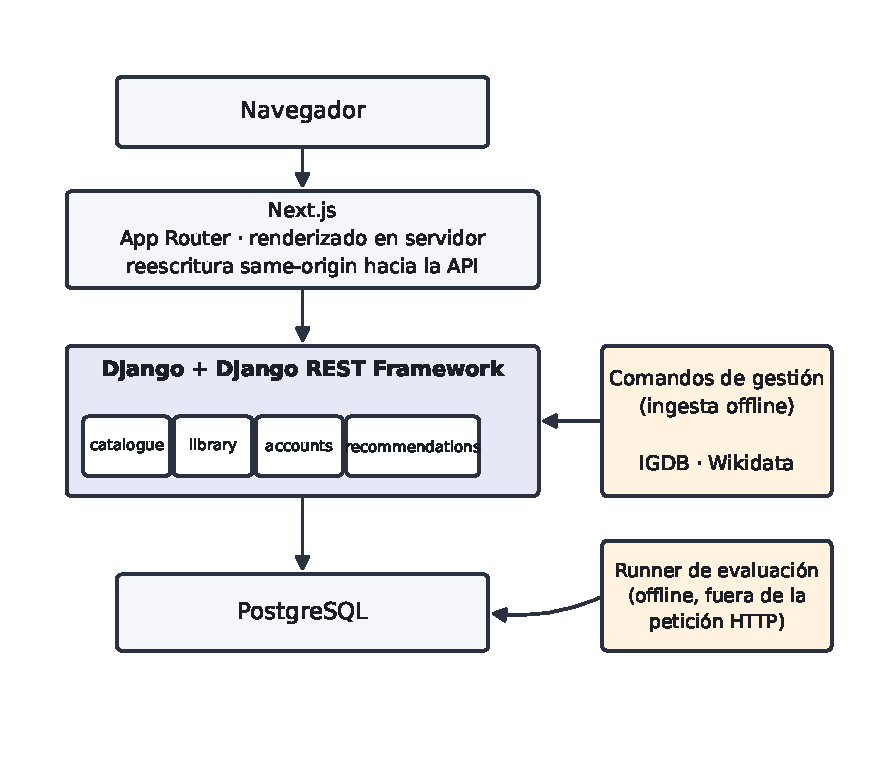
\includegraphics[width=0.8\textwidth]{figures/arquitectura.pdf}
    \caption[Arquitectura de SavePoint]{Arquitectura de SavePoint: el navegador solo habla con Next.js, que reescribe las llamadas hacia Django y DRF; los comandos de ingesta y el ejecutor de evaluación escriben en PostgreSQL fuera de la petición HTTP.}
    \label{fig:arquitectura}
\end{figure}

Esa elección no fue automática. El dominio de SavePoint (obras, ediciones, copias,
valoraciones, biblioteca) es relacional y con mucha escritura estructurada, el tipo de
problema para el que Django y su ORM están pensados desde el principio, con autenticación,
migraciones y validación ya resueltos en el propio marco de trabajo.
Frente a alternativas más ligeras como FastAPI con SQLAlchemy, que habrían obligado a componer
esas mismas piezas a mano, Django ofrece esa base madura sin coste adicional. Frente a servir
la interfaz con plantillas de Django y HTMX, que habría evitado duplicar el contrato de datos
entre backend y frontend, se prefirió un frontend Next.js separado porque el catálogo,
la biblioteca y las recomendaciones necesitaban una interfaz más rica de lo que las plantillas del
lado del servidor ofrecen con comodidad, sin perder por ello el renderizado en servidor que la
accesibilidad y el primer pintado rápido piden. Una arquitectura de microservicios, por
último, se descartó por su coste operativo y de trazabilidad en un proyecto de un único
desarrollador: separar servicios solo se justifica cuando hay una necesidad medida que lo
pida, no por anticipado.

PostgreSQL es la única base de datos de aplicación y de pruebas de integración, en desarrollo,
en pruebas y en despliegue, sin sustituir nunca por una base más ligera en ningún entorno. El
registro ADR-002 explica por qué: el modelo de datos de SavePoint depende de restricciones de
unicidad, de transacciones y de búsqueda por similitud de texto que SQLite soporta de forma
incompleta y que una base documental como MongoDB no ofrece con la misma garantía de
integridad relacional. Usar SQLite en local y PostgreSQL en producción, la solución más
barata a corto plazo, se descartó explícitamente porque introduce una asimetría entre entornos
que un banco de pruebas reproducible no se puede permitir: una consulta que funciona en SQLite
y falla en PostgreSQL, o viceversa, sería un defecto del propio diseño experimental, no del
código. Todo el sistema se levanta, en consecuencia, con Docker Compose a partir de los tres
componentes de aplicación (base de datos, API y frontend), cada uno construido desde su propio
fichero de Docker con versiones de dependencias fijadas; junto a ellos, Compose orquesta además un contenedor de \textit{worker} independiente por cada
variante de recomendación publicada (Sección~\ref{sec:alg-publicadas}). Un trabajo cuyo objeto
de estudio es la reproducibilidad de una comparación de algoritmos necesita, antes que nada,
que el propio entorno de ejecución sea reproducible y los contenedores eliminan esa variable
en cualquier máquina que lo levante.

Para el despliegue público se adoptó una topología repartida entre tres proveedores
gratuitos (Vercel para el frontend, Render para el backend y Neon para PostgreSQL), por una
restricción de partida no negociable: coste cero, sin tarjeta de pago. La
Sección~\ref{cap:despliegue}, en el capítulo de implementación, desarrolla esta topología,
sus límites conocidos y el estado actual del despliegue; el registro ADR-005 recoge la
decisión completa.

\section{Decisiones de arquitectura}\label{sec:dis-adr}

Cada decisión de diseño con consecuencias materiales queda registrada en \texttt{docs/adr/}
como ADR, con un formato fijo de contexto, alternativas,
decisión, evidencia, consecuencias, reversibilidad y aprobación. La
Tabla~\ref{tab:adr-resumen} resume el conjunto vigente; las secciones correspondientes citan
cada registro donde es relevante. Cada registro es citable y reversible: los límites de dominio
y las migraciones actúan como puntos de salida si una decisión se revisa.

\begin{table}[H]
\centering
\begin{tabularx}{\textwidth}{ | >{\raggedright\arraybackslash}p{0.14\textwidth} | Y | }
    \hline
    \textbf{Registro} & \textbf{Decisión y consecuencia principal} \\
    \hline
    ADR-001 & Monolito modular Django/DRF con frontend Next.js separado. Integridad y autenticación maduras, límites de dominio legibles, dos ejecutables con una sola arquitectura operable. \\
    \hline
    ADR-002 & PostgreSQL 18.6 como única base de datos de aplicación y de pruebas de integración. Paridad entre entornos, integridad relacional, bloqueos y búsqueda de trigramas disponibles de forma reproducible. \\
    \hline
    ADR-003 & Corpus congelado de Wikidata bajo dominio público y revisión de Commons por archivo. Evaluación repetible y procedencia visible, sin ninguna consulta a proveedores en tiempo de petición. \\
    \hline
    ADR-004 & Sesión de Django y frontera del mismo origen. Las primitivas de sesión y de protección contra falsificación de petición en sitios cruzados las mantiene Django; ningún token accesible al código del navegador. \\
    \hline
    ADR-005 & Docker Compose local y despliegue público repartido entre tres servicios gratuitos (Vercel, Render y Neon). Coste cero sin tarjeta, a cambio de que la aplicación cliente pública no sea la misma imagen que la local. \\
    \hline
    ADR-006 & IGDB como fuente del catálogo a escala real, con portadas por enlace directo. Cobertura real y modelado de género y plataforma de primera clase, a cambio de una obligación de atribución continua y de una licencia que es un acuerdo, no una dedicación al dominio público. \\
    \hline
    ADR-007 & Heurístico determinista de afinidad por géneros para la página de recomendaciones. Entrega el requisito como página real y explicable, deliberadamente al margen de la comparación sistemática de recomendadores que la Sección~\ref{cap:algoritmos} presenta más adelante. \\
    \hline
    ADR-008 & Valoraciones externas gobernadas por una versión inmutable versionada, con enriquecimiento acotado desde RAWG. \\
    \hline
    ADR-009 & Familias de algoritmos de recomendación y su ejecución como procesos trabajadores aislados. La web publica solo tres de las dieciséis variantes. \\
    \hline
\end{tabularx}
\caption{Registros de decisión de arquitectura vigentes.}
\label{tab:adr-resumen}
\end{table}

\section{Modelo de datos, API y sesión}\label{sec:dis-modelo-datos}\label{sec:dis-api}\label{sec:dis-sesion}\label{sec:dis-frontera}

El modelo de datos, descrito en la Sección~\ref{sec:req-informacion}, sigue cuatro decisiones
de diseño. La primera es que toda identidad canónica es un identificador único universal
(UUID) interno, generado en la importación, con el identificador del proveedor guardado solo
como procedencia; así, cambiar de proveedor o prescindir de él nunca obliga a renumerar el
catálogo (ADR-006, CAT-04). La segunda es que las restricciones y las transacciones viven
también en la base de datos, no solo en la capa de aplicación: unicidad de entrada por
persona y obra, unicidad de copia por clave de idempotencia, rango de la valoración por
restricción de comprobación y un disparador que impide que el cursor de importación de IGDB
retroceda. La tercera es la desnormalización deliberada de la fecha de primer lanzamiento y
de la valoración agregada sobre la propia obra, para que el filtrado por año y por nota sea
un recorrido de índice y no una agregación sobre cientos de miles de publicaciones. La cuarta
es un índice de trigramas sobre los alias normalizados, que sostiene la búsqueda tolerante
por prefijo y por similitud.


Las Figuras~\ref{fig:datos-catalogo}, \ref{fig:datos-biblioteca} y~\ref{fig:datos-social}
recogen el diagrama de entidades de ese modelo tal como lo implementan los modelos de Django.
A diferencia del modelo de dominio de la Figura~\ref{fig:modelo-dominio}, que solo nombra las
entidades, cada caja es una tabla con sus atributos más relevantes: \textit{PK} marca la clave
primaria, \textit{FK} una clave foránea, \textit{UQ} un atributo único y el signo de
interrogación un atributo que admite valores nulos. En cada línea, \texttt{N} aparece en el
extremo de la entidad que contiene la clave foránea y \texttt{1}, o \texttt{0..1} si la
referencia es opcional, en el extremo de la entidad referenciada. Las dimensiones del catálogo
(\texttt{Genre}, \texttt{Theme}, \texttt{Franchise}, \texttt{Developer}, \texttt{Publisher},
\texttt{GameMode}, \texttt{PlayerPerspective} y \texttt{Keyword}) se relacionan con la obra de
muchos a muchos y comparten una forma básica, por lo que se dibujan en una sola caja; las
etiquetas curadas lo hacen a través de la entidad de evidencia \texttt{GameWorkCuratedLabel}.
Cuando una entidad tiene dos claves foráneas hacia el usuario, como el remitente y el
destinatario de un mensaje, se dibuja una sola línea. Se omiten las entidades de importación y
de versionado del corpus, los subgéneros y las cuentas de demostración.

\begin{figure}[p]
    \centering
    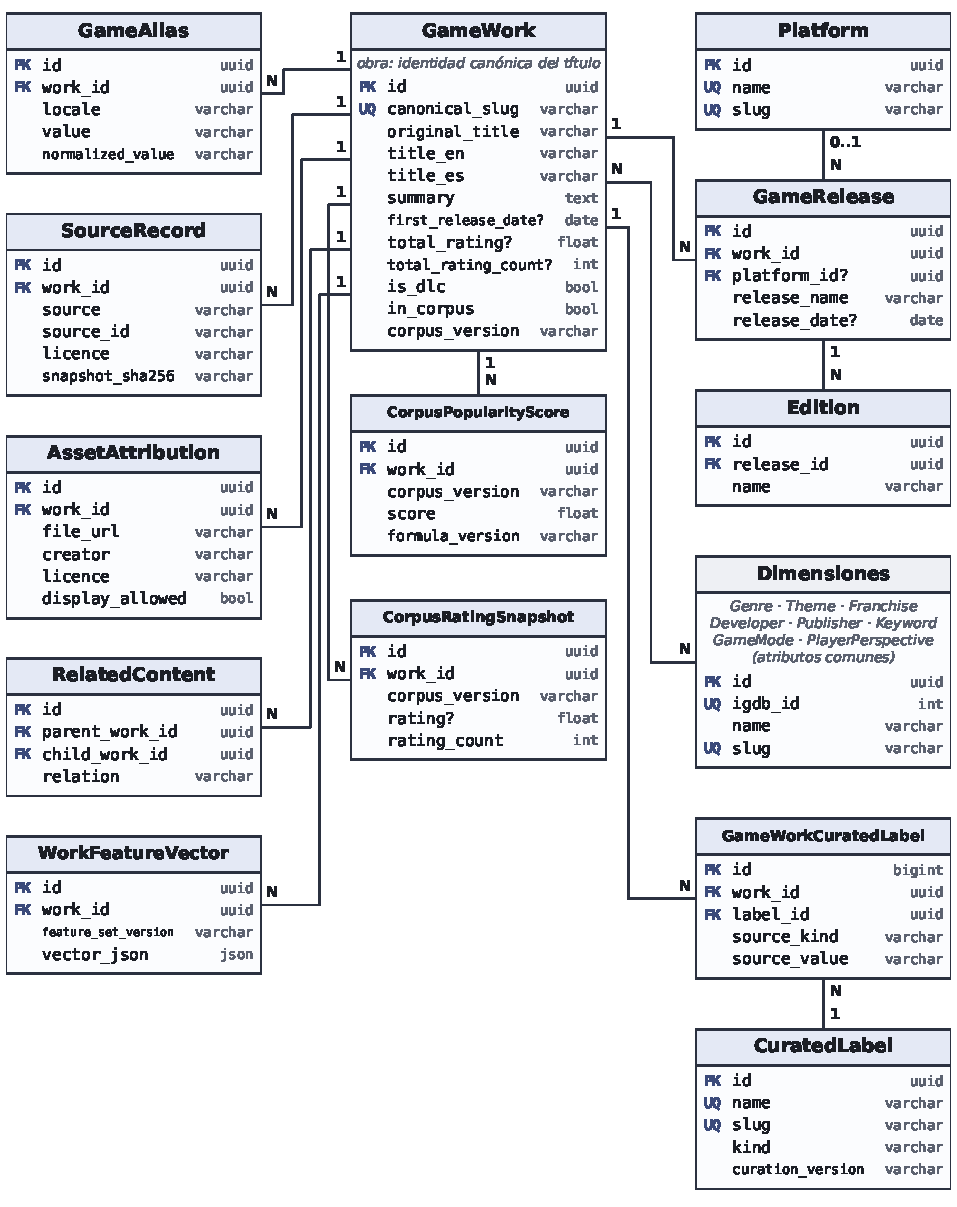
\includegraphics[width=\textwidth]{figures/modelo-datos-catalogo.pdf}
    \caption{Diagrama de entidades del catálogo, con las puntuaciones de corpus y el vector de características de cada obra.}
    \label{fig:datos-catalogo}
\end{figure}

\begin{figure}[p]
    \centering
    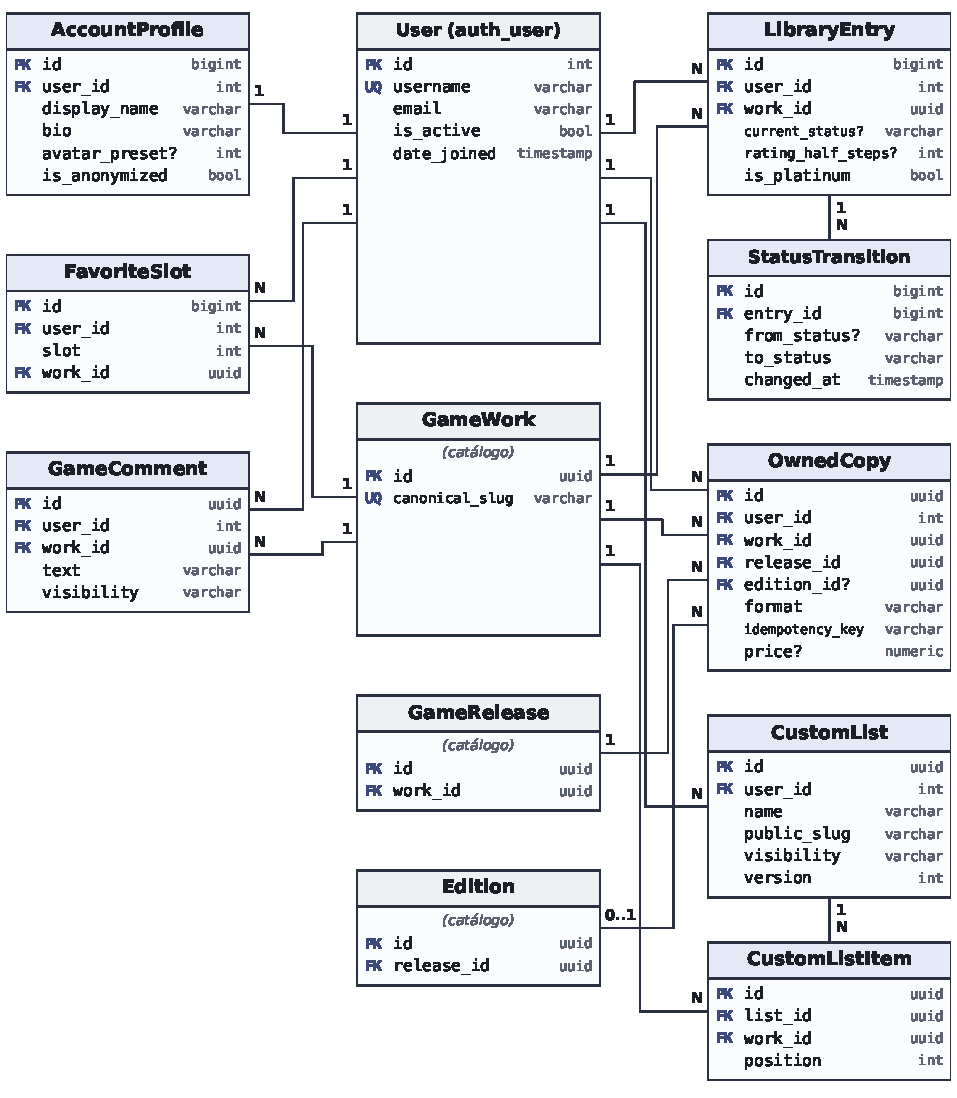
\includegraphics[width=\textwidth]{figures/modelo-datos-biblioteca.pdf}
    \caption[Diagrama de entidades de la biblioteca personal y de las cuentas]{Diagrama de entidades de la biblioteca personal y de las cuentas. \texttt{User}, \texttt{GameWork}, \texttt{GameRelease} y \texttt{Edition} se repiten con sus atributos mínimos como referencia.}
    \label{fig:datos-biblioteca}
\end{figure}

\begin{figure}[p]
    \centering
    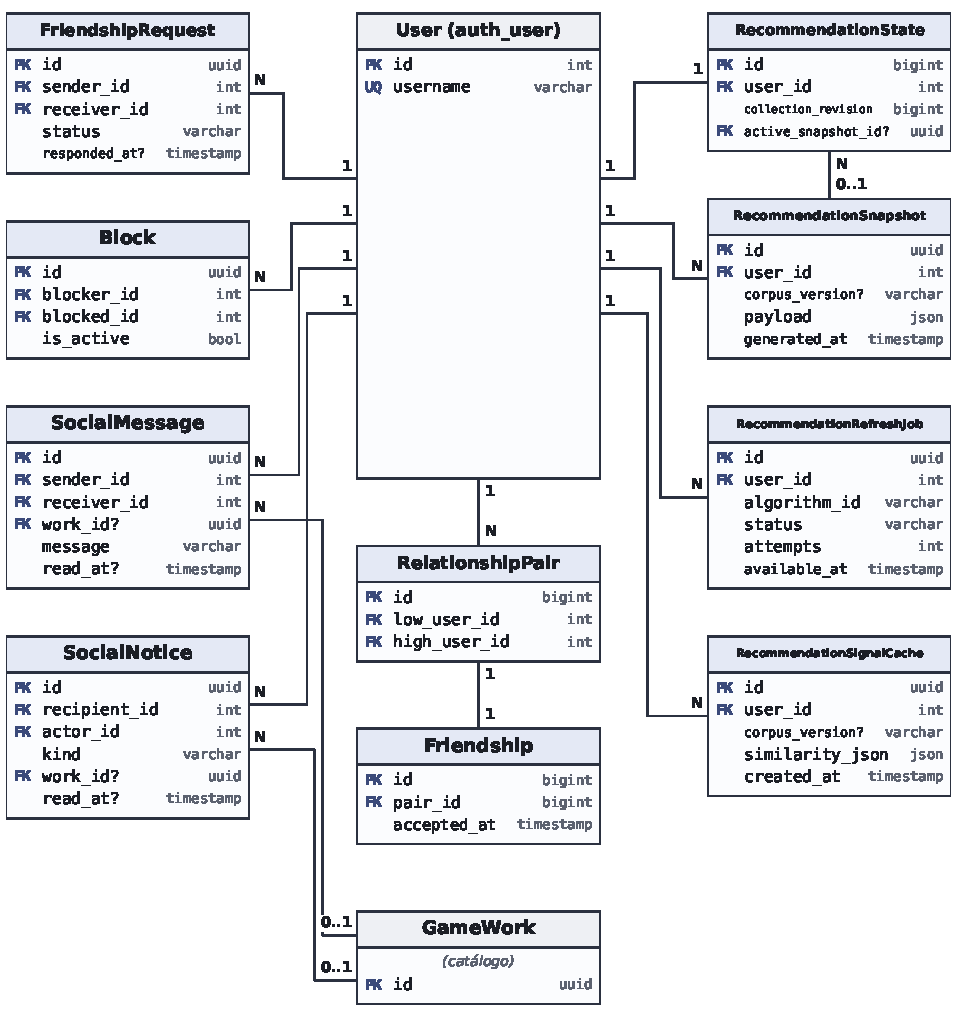
\includegraphics[width=\textwidth]{figures/modelo-datos-social.pdf}
    \caption{Diagrama de entidades de las amistades, los mensajes y las recomendaciones personalizadas.}
    \label{fig:datos-social}
\end{figure}

La API es de estilo de transferencia de estado representacional (REST), servida por DRF bajo el prefijo \texttt{/api/}. Las respuestas de
lista están paginadas. Las vistas de escritura y las de datos personales exigen sesión. Las
anónimas de mayor coste llevan un límite de ritmo con ámbito propio. La
Tabla~\ref{tab:endpoints} recoge los puntos de acceso principales.

\begin{table}[htbp]
\centering
\tablecompact
\begin{tabularx}{\textwidth}{ | L{0.39\textwidth} | C{0.12\textwidth} | Y | }
    \hline
    \textbf{Método y ruta} & \textbf{Acceso} & \textbf{Función} \\
    \hline
    \path{GET /api/catalogue/games/} & Anónimo & Lista paginada con búsqueda, filtros, orden y facetas. \\
    \hline
    \path{GET /api/catalogue/games/<slug>/} & Anónimo & Ficha de una obra con su jerarquía y su procedencia. \\
    \hline
    \path{GET /api/catalogue/sources/} & Anónimo & Dataset, licencia, hash y política de portadas. \\
    \hline
    \path{POST /api/accounts/login/}, \path{logout/} & Anónimo & Inicio y cierre de sesión con protección de origen. \\
    \hline
    \path{POST /api/accounts/register/} & Anónimo & Registro de nuevas personas usuarias, con límite de ritmo. \\
    \hline
    \path{GET /api/accounts/profiles/<alias>/} & Sesión & Perfil de un amigo aceptado, por lista de campos permitidos. \\
    \hline
    \path{GET/PUT/DELETE /api/accounts/me/avatar/} y \path{cover/} & Sesión & Foto de perfil y portada de la persona autenticada. \\
    \hline
    \path{POST /api/accounts/me/username/}, \path{password/} y \path{delete/} & Sesión & Cambio único del nombre de usuario, cambio de contraseña y eliminación de la cuenta. \\
    \hline
    \path{GET /api/social/notifications/} y \path{POST /api/social/messages/<id>/respond/} & Sesión & Notificaciones y respuesta a una recomendación recibida. \\
    \hline
    \path{GET /api/library/export/collection.xlsx} & Sesión & Exportación de la colección a Excel, además de en valores separados por comas (CSV). \\
    \hline
    \path{GET /api/library/entries/} & Sesión & Biblioteca de la persona autenticada. \\
    \hline
    \path{POST /api/library/entries/<id>/status/}, \path{rating/}, \path{copies/} & Sesión & Cambio de estado, valoración y alta de copias. \\
    \hline
    \path{GET /api/library/popularity/} & Anónimo & Recomendación de referencia por popularidad a partir de las señales importadas de IGDB. \\
    \hline
    \path{GET /api/recommendations/genre-taste/} & Sesión & Recomendación por afinidad de géneros de la persona autenticada. \\
    \hline
    \path{GET /api/recommendations/content/} y \path{snapshot/} & Sesión & Recomendaciones de una de las tres variantes publicadas y último conjunto completo de la persona, sin esperar al refresco. \\
    \hline
    \path{GET/POST /api/social/requests/} y \path{friendships/} & Sesión & Solicitudes de amistad, amistades y bloqueos. \\
    \hline
    \path{POST /api/library/import/preview/} y \path{apply/} & Sesión & Previsualización y aplicación de la importación de una colección. \\
    \hline
\end{tabularx}
\caption{Puntos de acceso principales de la API.}
\label{tab:endpoints}
\end{table}

La proyección de un perfil que ve un amigo se construye con una lista explícita de campos permitidos,
escrita a mano, en lugar de una serialización automática por introspección del modelo. Así,
exponer un campo privado nuevo requiere una decisión explícita, que es el modo de fallo
opuesto al de ocultarlo por olvido. Las imágenes de perfil y de portada se recortan y comprimen en el navegador, se limitan a 512~KiB, se validan en el servidor por su firma de formato y no por la extensión declarada y solo se sirven a su titular y a sus amigos aceptados. La eliminación de la cuenta exige la contraseña y deja un evento de auditoría sin actor, porque el registro de auditoría es de solo anexado.

La autenticación sigue el diseño del registro ADR-004. Django emite y valida la sesión. El
navegador solo llama a rutas del mismo origen de Next.js, que las reescribe hacia el backend
mediante una variable de entorno visible únicamente en el servidor. Las cookies de sesión y
de protección contra falsificación de petición en sitios cruzados (CSRF) viajan con ámbito
del mismo origen, sin necesidad de compartir recursos entre orígenes con credenciales. Las
mutaciones exigen el testigo CSRF. El cierre de sesión la invalida. Los redirectos
posteriores al acceso solo aceptan rutas relativas del mismo sitio, revalidadas en el
servidor. No hay ningún testigo de tipo \textit{bearer} accesible al código JavaScript del
navegador.

El diseño mantiene dos fronteras explícitas. Ninguna cuenta es pública, de modo que solo los
amigos aceptados acceden a su contenido y el acceso a IGDB está confinado a un comando de
gestión fuera de línea, sin que ninguna petición de usuario llame a un proveedor externo
(RN-8 y RN-9 de la Tabla~\ref{tab:reglas-negocio}).

\section{Diseño de la interfaz de usuario}\label{sec:dis-ui}

El diseño de la interfaz se fijó en un contrato de diseño, \texttt{01.1-UI-SPEC.md},
aprobado antes de implementar y validado por un subagente comprobador. El contrato define un
sistema de tokens de diseño en variables de hojas de estilo en cascada (CSS), con juegos completos para tema claro y tema oscuro, cuya
selección se aplica en el servidor mediante una cookie para evitar el destello al cargar. Los
componentes reutilizables incluyen la tarjeta de juego, las píldoras de estado y de nota, la
valoración por estrellas, la imagen de portada con su marcador de reserva, la barra de
filtros, el conmutador de tema y el menú de cuenta. Las Figuras~\ref{fig:ui-claro}
y~\ref{fig:ui-oscuro} muestran la página de inicio en ambos temas. La franja inferior de ambas
recoge las cifras del catálogo de la instalación local, que son las del corpus gobernado
\texttt{2026.09.2} descrito en la Sección~\ref{sec:datos-congelacion}: 190.479 obras, de las que
30.695 tienen nota de IGDB.

\begin{figure}[H]
    \centering
    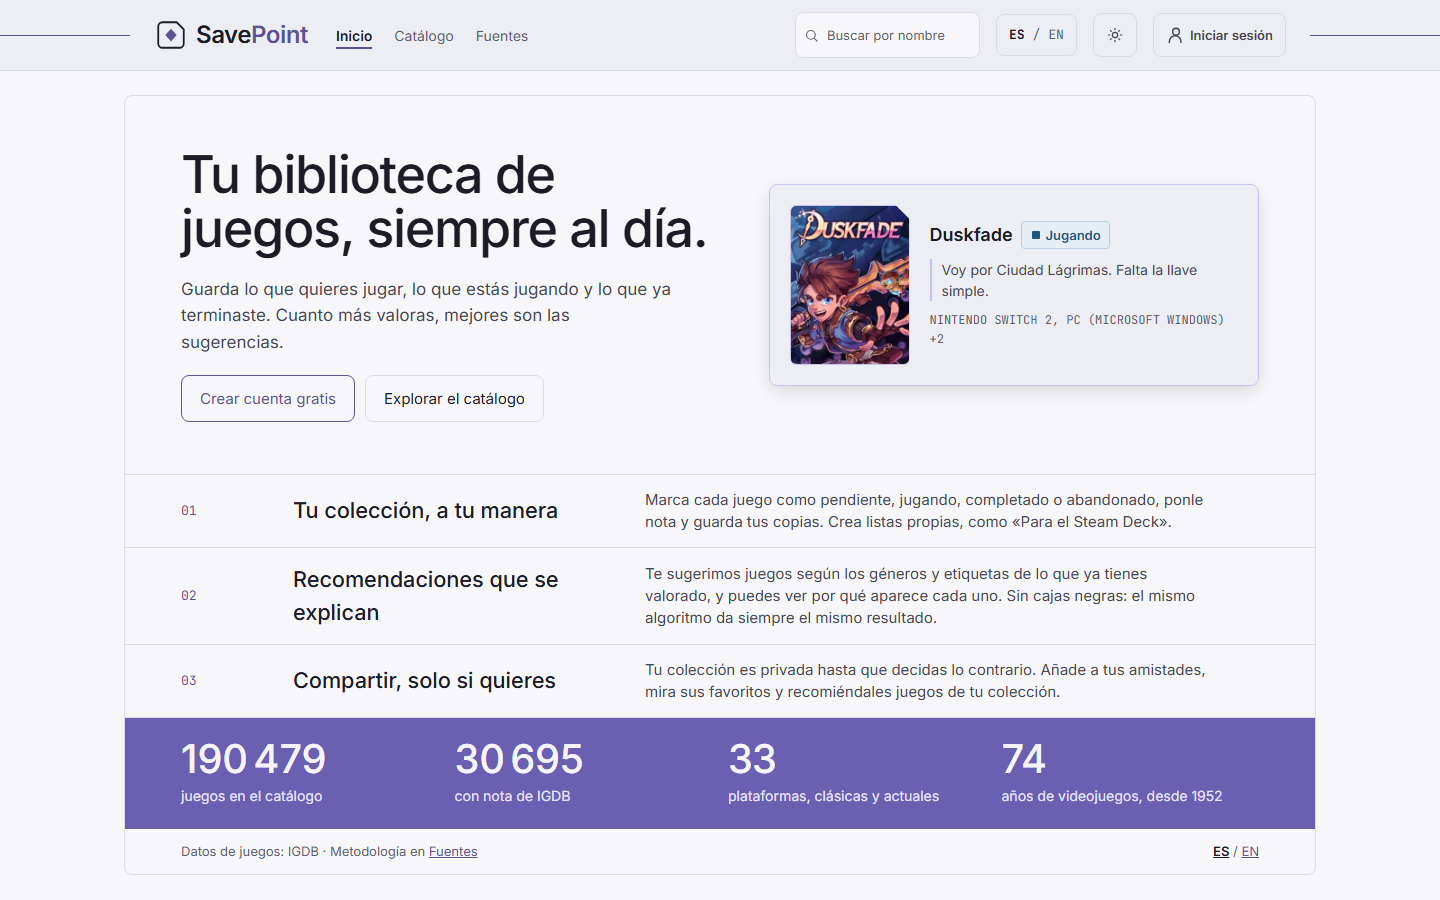
\includegraphics[width=0.85\textwidth]{figures/01-inicio-claro.png}
    \caption{Página de inicio con tema claro y sin sesión iniciada.}
    \label{fig:ui-claro}
\end{figure}

\begin{figure}[H]
    \centering
    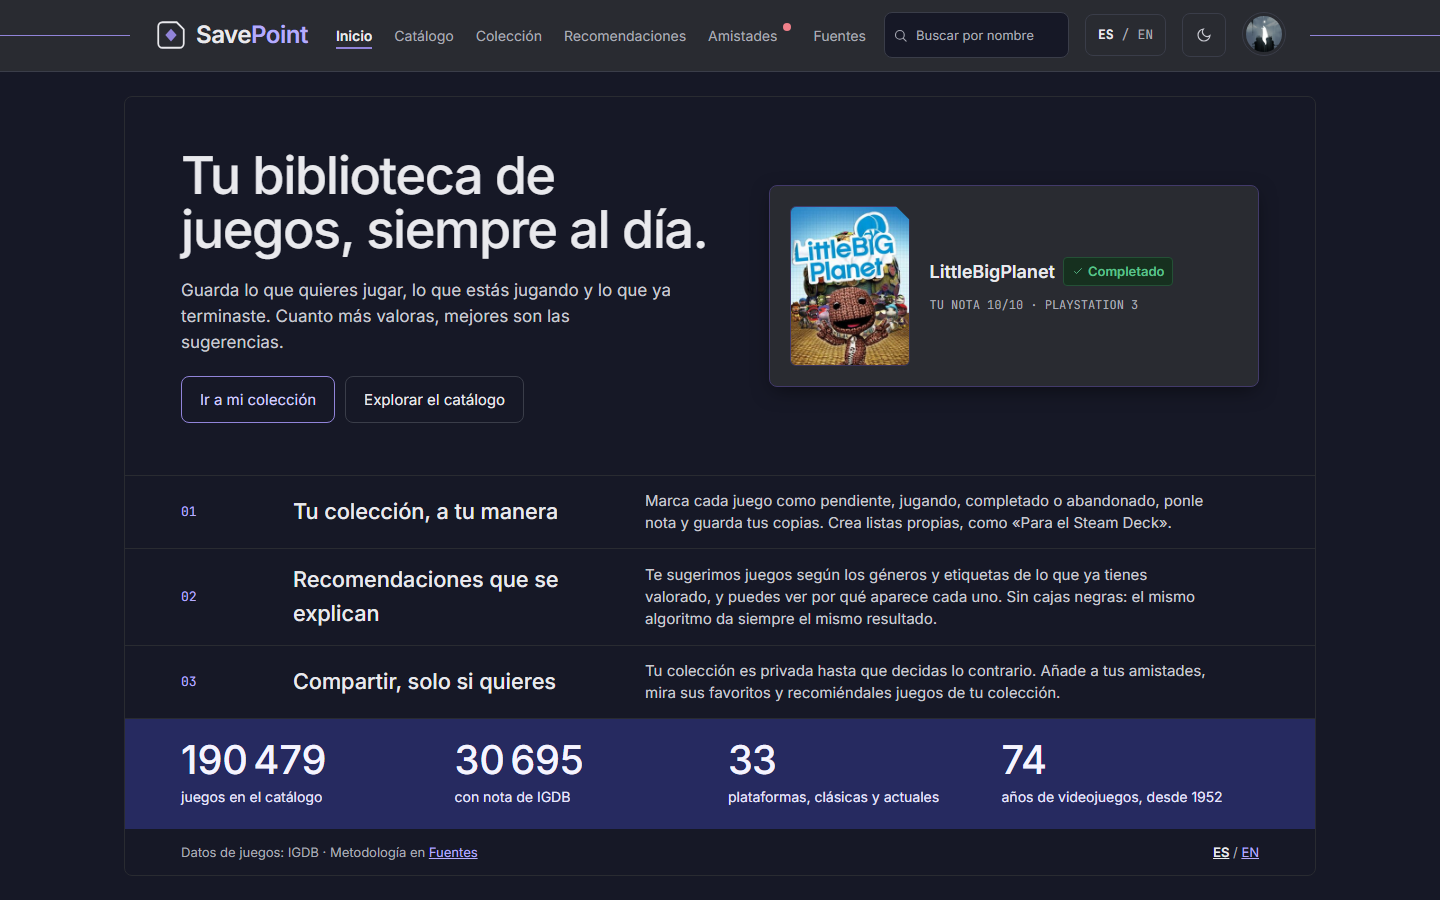
\includegraphics[width=0.85\textwidth]{figures/01-inicio-oscuro.png}
    \caption{Página de inicio con tema oscuro y con sesión iniciada.}
    \label{fig:ui-oscuro}
\end{figure}

El contrato de diseño incluye una matriz de cobertura por superficie, con filas para el
catálogo, el detalle, el registro y las recomendaciones, cada una con su verificación en
escritorio, en móvil y de accesibilidad. El Capítulo~\ref{cap:implementacion} describe las
rutas y los componentes concretos; la Sección~\ref{cap:pruebas} recoge su verificación.

\section{Diseño de los algoritmos de recomendación}\label{cap:algoritmos}\label{cap:nucleo-investigacion}

Esta sección detalla cómo SavePoint representa una obra y a una persona usuaria, qué señales
intervienen en la puntuación de una candidata, con qué fórmulas y pesos exactos se combinan esas
señales en cada uno de los dieciséis algoritmos comparados, qué respaldo en la literatura tiene cada
una de esas decisiones y cuáles se descartaron y por qué. El Capítulo~\ref{cap:resultados}
somete después esos algoritmos al protocolo de evaluación sin conexión y presenta los resultados
obtenidos.

Conviene separar desde el principio dos planos que se confunden con facilidad. La literatura
avala las \emph{familias} de técnicas empleadas y los \emph{principios} de ponderación,
similitud, vecindad, hibridación, diversificación y medición; no convierte en constantes
universales los valores numéricos concretos que este proyecto fija. Los pesos por familia de
faceta, el parámetro \(\beta\) de la media F, el factor de contracción de la valoración, los pesos de
estado de biblioteca, el umbral de evidencia negativa, el \(\lambda\) de la reordenación y los
cortes \(K\) son decisiones explícitas de diseño para este corpus y este trabajo, tomadas y
documentadas como tales, no resultados heredados de una publicación. Cada apartado indica qué
parte pertenece a cada plano.

Los resultados publicados proceden de la ejecución \texttt{evaluation-400-test-2026-09-12-v15},
que su propio artefacto registra con el protocolo 15 y el conjunto de características
\texttt{fs-v12-curated-tags-idf}. Conviene no confundir las dos numeraciones, que son
independientes: el \emph{protocolo} de evaluación (v12, v14 y v15 son los tres que se ejecutaron
hasta el final, Sección~\ref{sec:exp-evolucion}) define cómo se mide y el \emph{conjunto de
características} (\texttt{fs-v12}, \texttt{fs-v13}) define cómo se representa cada obra, de modo
que v12 y \texttt{fs-v12} no designan lo mismo. Después de esa ejecución, la revisión de los pesos
reales sobre el corpus llevó a \texttt{fs-v13-family-weighted-tags}, que corrige el reparto de
peso entre familias de etiquetas (descrito más abajo) y con el que el código vigente funciona
bajo el protocolo 16. Todavía no se ha ejecutado ni publicado una evaluación completa con
\texttt{fs-v13}. Por eso este apartado describe la implementación vigente (\texttt{fs-v13}),
mientras que todas las cifras del Capítulo~\ref{cap:resultados} corresponden a \texttt{fs-v12};
la Tabla~\ref{tab:pesos-familia} recoge los pesos de ambas versiones y ninguna métrica
publicada de v15 se recalcula ni se reinterpreta.

\subsection{Representación de una obra y del perfil de la persona usuaria}\label{sec:alg-representacion}

La arquitectura de recomendación basada en contenido que sigue el sistema (describir cada ítem
con un conjunto de rasgos, construir un perfil de intereses a partir del historial de la
persona y comparar ambos para ordenar candidatas) es la formulación clásica de la familia,
descrita por Pazzani y Billsus~\cite{pazzani2007content}. Lo que este trabajo decide por su
cuenta es qué rasgos concretos describen un videojuego, cómo se curan y con qué intensidad
participa cada entrada de la biblioteca.

Una candidata para recomendar debe ser una obra gobernada del corpus (190.479 en la versión
\texttt{2026.09.2} con la que se evaluó, Sección~\ref{sec:datos-congelacion}), no contenido
descargable, publicada antes de la fecha de corte, con valoración externa disponible y al
menos cinco valoraciones agregadas; también se excluye cualquier obra que ya aparezca en la
biblioteca de la persona. Estas exclusiones impiden recomendar una posesión ya conocida,
lanzar contenido todavía no publicado o amplificar una nota sostenida por evidencia
insuficiente.

Cada obra se representa mediante un vector disperso de familias de facetas: etiquetas de
género y subgénero curadas, tema, característica, modo, franquicia, desarrollador y
plataforma. Los géneros y subgéneros forman el núcleo semántico de la representación; tema,
característica, modo, franquicia y desarrollador actúan como confirmaciones opcionales; la
plataforma expresa compatibilidad material más que afinidad de gusto. Las palabras clave,
perspectivas y modos crudos que ofrece la fuente de datos no se introducen directamente en el
vector: tienen ruido, sinónimos y semánticas heterogéneas, de modo que solo entran tras una
curación editorial que elimina duplicados y unifica niveles. Una faceta ausente en una obra se
omite sin más; el sistema nunca imputa ni redistribuye su peso a otra familia, porque hacerlo
premiaría la escasez de metadatos en lugar de ser neutral ante ella.

Dentro de cada familia, el peso de un valor concreto (por ejemplo, el género \texttt{rpg} o el
tema \texttt{cyberpunk}) se calcula con una frecuencia inversa de documento (IDF) suavizada, de modo
que un valor raro dentro de su propia familia pese más que uno común. El fundamento es la
ponderación estadística de términos y la representación vectorial dispersa de Salton y
Buckley~\cite{salton1988term}: los rasgos que aparecen en casi todos los documentos
discriminan poco y los infrecuentes discriminan mucho. Desde la revisión \texttt{fs-v13}, cada
familia calcula su rareza sobre su propio universo de referencia, no sobre el corpus gobernado
completo: si \(N_f\) es el número de obras gobernadas con algún valor de la familia \(f\) y
\(df_t\) el número de esas obras que contienen el valor \(t\),

\begin{equation}\label{eq:idf}
idf(t) = \ln\!\left(\frac{N_f + 1}{df_t + 1}\right) + 1 ,
\end{equation}

con suavizado aditivo de \(1\) para mantener un valor finito incluso para un valor observado
en una única obra. La versión anterior, \texttt{fs-v12}, no separaba las familias: género,
subgénero, tema, modo y característica compartían un único presupuesto fusionado
(\(\mathtt{tag}=0{,}75\)) con un solo cálculo de IDF entre las cinco. Eso permitía que un
subgénero raro pesara más que el propio género por pura rareza estadística del conjunto
fusionado. La plataforma pesaba entonces 0,25, con un reparto plano \(1/\sqrt{k}\), en lugar
del 0,05 y del IDF propio que le da \texttt{fs-v13}. Una primera corrección, renormalizar las cinco familias juntas sin separarlas,
se descartó porque terminaba premiando a las obras con menos metadatos en lugar de corregir el
sesgo. La solución adoptada en \texttt{fs-v13} fue separar cada familia en su propio cálculo de
IDF, con su propio universo de referencia \(N_f\) y su propio peso (\(\mathtt{tag}=0{,}60\),
que fusiona género y subgénero; \(\mathtt{theme}=0{,}20\); \(\mathtt{feature}=0{,}10\);
\(\mathtt{mode}=0{,}05\); \(\mathtt{platform}=0{,}05\)), de modo que la rareza de un valor se
mide siempre dentro de la población que realmente lo declara, no contra un denominador
compartido con familias de cobertura muy distinta. La fórmula procede de la literatura; el
cálculo de \(df\) sobre obras gobernadas, el suavizado y los pesos por familia son adaptaciones
reproducibles a este corpus. Franquicia
y desarrollador no usan IDF: si una obra declara \(k\) valores observados de esa familia, cada
uno pesa \(1/\sqrt{k}\), un reparto plano que evita premiar la rareza de un estudio o de una
saga, señales de cobertura desigual en las que una coincidencia rara diría más del catálogo que
del gusto de la persona.

Si \(T\) es el conjunto de valores que una obra declara en la familia \(f\), el peso de la
coordenada correspondiente a un valor \(t\) es

\begin{equation}\label{eq:facet-weight}
w(f{:}t) = W_f \cdot \frac{idf(t)}{\sqrt{\sum_{q \in T} idf(q)^2}} ,
\end{equation}

donde \(W_f\) es el peso fijo asignado a la familia \(f\) (Tabla~\ref{tab:pesos-familia}, columna
\texttt{fs-v13} para la implementación vigente) y la
normalización L2 en el denominador, también procedente del modelo vectorial
clásico~\cite{salton1988term}, evita que una obra gane afinidad solo por declarar más valores
dentro de la misma familia. El reparto concreto de \(W_f\) es, en cambio, una decisión de
producto: prioriza la semántica de género sobre la compatibilidad de plataforma, que se
mantiene como una restricción y no como una afinidad. Igualar ambos pesos se consideró y se
descartó por ese mismo motivo.

\begin{table}[H]
\centering
\caption[Peso fijo de cada familia de faceta en el vector de contenido]{Peso fijo \(W_f\) de cada familia de faceta en el vector de contenido, en
\texttt{fs-v12} (versión con la que se calcularon los resultados del
Capítulo~\ref{cap:resultados}) y en \texttt{fs-v13} (implementación vigente). En
\texttt{fs-v12}, \texttt{tag} reunía género, subgénero, tema, característica y modo en un único
peso; en \texttt{fs-v13} agrupa solo género y subgénero. El valor \enquote{n/d} indica que la familia no
existía por separado. Los valores son una decisión de diseño de SavePoint, no una constante de
la literatura.}\label{tab:pesos-familia}
\begin{tabularx}{\textwidth}{@{}Yrr@{}}
\textnormal{Familia} & \textnormal{\texttt{fs-v12}} & \textnormal{\texttt{fs-v13}} \\
\hline
Etiqueta (\texttt{tag}) & 0,75 & 0,60 \\
Plataforma (\texttt{platform}) & 0,25 & 0,05 \\
Tema (\texttt{theme}) & n/d & 0,20 \\
Característica (\texttt{feature}) & n/d & 0,10 \\
Modo (\texttt{mode}) & n/d & 0,05 \\
Franquicia (\texttt{franchise}) & 0,02 & 0,02 \\
Desarrollador (\texttt{developer}) & 0,015 & 0,015 \\
\end{tabularx}
\end{table}

El perfil de contenido de una persona usuaria se construye únicamente a partir de sus
entradas de biblioteca terminadas o en curso con valoración personal de al menos siete medios
puntos sobre diez; una entrada con valoración inferior a ese umbral no se añade al perfil
positivo, sino que alimenta un perfil de evidencia negativa aparte. Cada entrada \(i\) aporta
un peso de actividad \(entry\_weight_i = status\_weight_i + r_i^2\), donde \(status\_weight\)
vale 3 para una obra terminada, 2 para una obra en curso, 1 para pendiente y 0 para abandonada
y \(r_i\) es la valoración personal normalizada a \([0,1]\). Elevar la valoración al cuadrado
hace que una nota alta cuente como evidencia bastante más intensa que una simplemente
positiva. Esta forma de modular la contribución de cada ítem del historial es la aplicación
directa del principio de perfil ponderado por interés de la familia basada en
contenido~\cite{pazzani2007content}; los valores 3, 2, 1 y 0 y el exponente cuadrático son
decisión local. El perfil es la media ponderada de los vectores normalizados de las entradas
elegibles y no se vuelve a normalizar globalmente después; conserva así la intensidad relativa
acumulada de la biblioteca. Cuando una etiqueta se repite en al menos tres entradas de baja
valoración, se activa como evidencia negativa. Ese umbral de tres es deliberado: una
penalización sin umbral convertiría una única experiencia mal valorada en un rechazo estable,
que es precisamente el error que se quería evitar. Con menos de tres entradas positivas
elegibles, o sin ningún vector de características disponible, el sistema entra en un modo explícito de
historial insuficiente: no inventa un perfil ni recurre silenciosamente a la biblioteca de otra
persona; esa limitación queda declarada así en la respuesta.

\subsection{Similitud de contenido y señales escalares de la candidata}\label{sec:alg-similitud}

La similitud entre el perfil de una persona y una obra candidata no aplica el coseno
ciegamente sobre todo el vector. Para cada familia se calculan por separado la cobertura del
perfil y la precisión de la candidata: si \(P_f\) y \(C_f\) son los valores de perfil y
candidata en la familia \(f\) y \(O_f = P_f \cap C_f\) su solapamiento,

\[
cobertura_f = \frac{\sum_{t \in O_f} P_f[t]}{\sum_{t \in P_f} P_f[t]}, \qquad
precision_f = \frac{|O_f|}{|C_f|} ,
\]

y ambas cantidades se combinan con una media \(F_\beta\) con \(\beta = 0{,}5\),

\begin{equation}\label{eq:fbeta}
F_{0{,}5} = \frac{(1+0{,}5^2)\;cobertura \cdot precision}{0{,}5^2 \cdot precision + cobertura} .
\end{equation}

La media \(F_\beta\) como forma canónica de equilibrar precisión y cobertura con un único
parámetro procede de van Rijsbergen~\cite{vanrijsbergen1979information}; el valor
\(\beta = 0{,}5\) es la decisión local y da más peso a la precisión de la candidata que a la
cobertura del perfil, de modo que una obra que declara muchos valores de una familia no gana
automáticamente por enumerar más. Se consideraron dos alternativas y se descartaron por
motivos concretos: una media aritmética simple favorece a las candidatas con más metadatos
declarados y el coseno puro sobre el vector completo, aunque más habitual, resulta menos
separable a la hora de explicar por qué se recomienda una obra y más vulnerable a las
candidatas con muchas facetas.

En \texttt{fs-v13}, el núcleo renormalizado de la similitud se limita a las dos familias con
cobertura casi universal, etiqueta y plataforma, ponderadas exactamente con los pesos
\(W_{tag}=0{,}60\) y \(W_{platform}=0{,}05\) de la Tabla~\ref{tab:pesos-familia} (en
\texttt{fs-v12} el núcleo estaba formado por las mismas dos familias, con \(W_{tag}=0{,}75\) y
\(W_{platform}=0{,}25\)):

\[
nucleo = \frac{\sum_{f \in \{tag,\,platform\}} W_f \cdot F_{0{,}5,f}}{\sum_{f \in \{tag,\,platform\}} W_f \text{ activos}} .
\]

Las cinco familias restantes (tema, característica, modo, franquicia y desarrollador) suman
un bono de confirmación acotado, fuera de ese núcleo, que nunca resta ni se redistribuye
cuando una familia falta en cualquiera de los dos lados:

\begin{equation}\label{eq:bonus}
\begin{split}
bono ={}& 0{,}20\,aff_{tema} + 0{,}10\,aff_{caracteristica} + 0{,}05\,aff_{modo}\\
      &+ 0{,}02\,aff_{franquicia} + 0{,}015\,aff_{desarrollador} ,
\end{split}
\end{equation}

con \(aff_f = \min\!\big(1,\, \sum_{t \in O_f} P_f[t] / \max_{t \in P_f} P_f[t]\big)\) y la
similitud final \(similitud = \min(1,\ nucleo + bono)\). Esta asimetría entre núcleo y bono es
deliberada: un tema, una saga o un estudio confirman un interés ya observado en el género o la
plataforma, pero no deben sustituir esa similitud semántica ni inflarla artificialmente cuando
falta información secundaria. Situar franquicia o desarrollador en el núcleo se descartó por su
cobertura desigual y por el riesgo de recomendar por coincidencia superficial de editor más que
por afinidad real. El coseno completo sobre el vector no desaparece: se reserva para medir la
redundancia entre recomendaciones y la diversidad intra-lista de las variantes con
reordenación, donde su interpretación geométrica directa sí es exactamente la propiedad
necesaria.

La calidad externa de una candidata no usa su valoración agregada en bruto, sino que se
estabiliza con contracción bayesiana hacia la media del corpus, para que una
nota extrema sostenida por pocas observaciones no domine el resultado. El fundamento es el
principio de Empirical Bayes: las observaciones escasas se contraen hacia un prior común para
reducir la varianza del estimador~\cite{efron2010large}. Con \(n\) valoraciones observadas,
prior del corpus \(\mu\) (la media de valoraciones ponderada por su propio volumen de votos) y
un parámetro de contracción \(m=25\),

\[
valoracion_{bayes} = \frac{n \cdot valoracion + m\,\mu}{n+m}, \qquad
rating_{final} = \left(\frac{rating_{bayes}}{100}\right)^{2} \cdot \frac{n}{n+m} .
\]

El valor \(m=25\), el exponente cuadrático sobre la nota normalizada y el factor de confianza
\(n/(n+m)\) son, de nuevo, decisiones locales: el cuadrado separa mejor a las candidatas de
calidad alta y el factor de confianza penaliza de forma explícita el volumen de evidencia, no
solo la nota media. Usar la valoración en bruto se descartó por el sesgo evidente de las notas
extremas con poca evidencia y volver a multiplicar por el volumen de votos también, porque ese
volumen ya participa una vez dentro de la propia contracción. Cuando una candidata no tiene
valoración externa propia observada, el sistema recurre a la mediana de valoración de sus
etiquetas curadas y marca el resultado como una aproximación, sin presentarlo como una
observación real.

La popularidad externa (\emph{PopScore}) tampoco usa el valor bruto de la fuente de datos: su
escala es larga y arrastra un sesgo de popularidad conocido, así que cada una de sus cuatro
primitivas se transforma con \(\log(1+x)\) y después se convierte en un percentil de rango
dentro de la versión inmutable congelada, combinándose como \(PopScore = 0{,}40\,\text{Visitas} +
0{,}25\,\text{Jugando} + 0{,}25\,\text{Jugado} + 0{,}10\,\text{Quiere jugar}\). Si falta
cualquier primitiva, no existe composición observada y las variantes que la consumen aplican un
suelo explícito de cero, marcado como tal, sin redistribuir el peso que le correspondía. La
recencia, por último, solo es estimable para una obra con fecha de lanzamiento no futura: con
\(year\_gap\) el número de años naturales transcurridos desde su publicación hasta la fecha de
corte, \(recency = 0{,}35^{\,year\_gap}\), de modo que una obra del año del corte vale
\(1{,}0\), una del año anterior \(0{,}35\) y así sucesivamente. Se eligió una base geométrica
sobre años naturales en lugar de una semivida diaria porque esta última es menos interpretable
y depende del día exacto del corte, lo que la haría frágil ante una repetición del experimento
en otra fecha.

\subsection{Las tres familias y sus dieciséis variantes}\label{sec:alg-familias}

Con la afinidad de contenido \(C\), la calidad \(R\), la popularidad \(P\), la evidencia
negativa \(N\) y la recencia \(X\) ya definidas, la Tabla~\ref{tab:variantes-contenido} recoge
la fórmula exacta de las diez variantes basadas en contenido y de la de recencia, incluidas las dos con
reordenación por relevancia marginal máxima (\textit{maximal marginal relevance}, MMR). Todas comparten el mismo conjunto
de candidatas, el mismo vector de características y el mismo perfil de usuario; lo único que cambia
entre ellas es cómo combinan sus señales, precisamente para que la comparación aísle esa
decisión de diseño y no otra.

\begin{table}[H]
\centering
\caption{Fórmula de combinación de las diez variantes basadas en contenido y de la de recencia.}\label{tab:variantes-contenido}
\small
\begin{tabularx}{\textwidth}{@{}>{\ttfamily\raggedright\arraybackslash}p{0.48\textwidth}>{\raggedleft\arraybackslash}X@{}}
\textnormal{Algoritmo} & \textnormal{Fórmula} \\
\hline
content-cbf-weighted-v1 & \(S = 0{,}70\,C + 0{,}30\,R\) \\
content-cbf-multiplicative-v1 & \(S = C \cdot R\) \\
content-cbf-twostage-v1 & \(b=\min(4,\lfloor 5C\rfloor);\ S = b + R/6\) \\
content-cbf-neg-v1 & \(S = \max(0,\ 0{,}70C + 0{,}30R - N)\) \\
content-cbf-weighted-pop-v1 & \(S = 0{,}55C + 0{,}25R + 0{,}20P\) \\
content-cbf-multiplicative-pop-v1 & \(S = C \cdot R \cdot (0{,}80 + 0{,}40P)\) \\
content-cbf-twostage-pop-v1 & \(b=\min(4,\lfloor 5C\rfloor);\ S = b + (0{,}80R+0{,}20P)/6\) \\
content-cbf-neg-pop-v1 & \(S = \max(0,\ 0{,}55C + 0{,}25R + 0{,}20P - N)\) \\
recency-v1 & \(S = 0{,}20C + 0{,}20R + 0{,}20P + 0{,}40X\) \\
content-cbf-mmr-v1 / -pop-v1 & MMR sobre Weighted / Weighted-Pop \\
\end{tabularx}
\end{table}

La existencia de estas variantes no responde a un afán de acumular algoritmos, sino al
diseño experimental: cada una aísla una única decisión de combinación manteniendo constantes
las candidatas, las características y las versiones inmutables, de modo que una diferencia de resultado se pueda
atribuir a esa decisión concreta. \texttt{content-cbf-weighted-v1} actúa como referencia del
grupo porque sus pesos son explícitos y su comportamiento es fácil de explicar: el contenido
domina la puntuación y la calidad ordena dentro de un mismo nivel de afinidad. La variante
multiplicativa exige afinidad y calidad simultáneamente, sin que una compense a la otra. La de
dos etapas usa la afinidad para asignar una banda discreta y solo desempata dentro de ella con
la calidad, de modo que una nota alta nunca rescata una afinidad baja. La negativa resta la
evidencia de rechazo acumulada sobre las mismas etiquetas. Las cuatro variantes con sufijo
\texttt{-pop} repiten exactamente esas combinaciones incorporando además un veinte por ciento
de PopScore, con el resto de pesos reescalados para que la suma se mantenga acotada; en la
multiplicativa, un PopScore nulo produce un factor \(0{,}80\) y uno máximo un factor
\(1{,}20\), un ajuste acotado y nunca una sustitución de la afinidad de contenido.
\texttt{recency-v1} reparte su peso entre las cuatro señales con un cuarenta por ciento para la
novedad, lo que la convierte en una variante de descubrimiento sin abandonar del todo la
personalización.

Fuera de la familia de contenido, \texttt{cf-user-knn-v1} implementa el filtrado colaborativo
por vecindad de usuarios en la forma que introdujeron Resnick y otros en
GroupLens~\cite{resnick1994grouplens} y que sistematizaron Herlocker y
otros~\cite{herlocker2004evaluating}: similitud entre personas calculada sobre las obras que
ambas han valorado, valoraciones centradas por la media de cada persona y predicción por
agregación ponderada de las desviaciones de los vecinos. Las decisiones locales son el mínimo
de dos obras co-valoradas para considerar fiable una vecindad y el máximo de veinte vecinos con
similitud positiva. Es explicable por los vecinos y las obras que comparten, pero sufre
arranque en frío: con historial escaso, o sin vecindad suficiente, no puede inferir una
preferencia colaborativa fiable. Se descartó implementar en su lugar un colaborativo por
vecindad de ítems porque exige construir una matriz ítem-ítem y descansa sobre otra hipótesis
de generalización, mientras que la vecindad de usuarios resulta más legible con la valoración
explícita disponible en este corpus.

El híbrido responde al argumento de Burke~\cite{burke2002hybrid}: combinar fuentes
complementarias permite aprovechar las ventajas de cada una y compensar sus debilidades. Su
combinación es \(H(i) = 0{,}60\,\mathit{Weighted}(i) + 0{,}40\,\mathit{CF}(i)\); si el
componente colaborativo no dispone de historial suficiente, el híbrido conserva la relevancia
de contenido y declara la alternativa de respaldo en lugar de penalizar artificialmente a una persona
nueva. El reparto 0,60/0,40 es en sí mismo una decisión local sujeta a evaluación, no una regla
tomada de la literatura.

Las dos variantes con reordenación por diversidad aplican la MMR
tal como la formularon Carbonell y Goldstein~\cite{carbonell1998mmr}: recorren un conjunto de
tamaño \(\max(100, 5K)\) y en cada posición eligen la candidata que maximiza
\(\lambda\,Rel(i) - (1-\lambda)\max_{j \in S} cosine(i,j)\), con \(Rel(i)\) la relevancia ya
calculada y \(S\) la lista parcial ya elegida. El valor \(\lambda = 0{,}80\) y el tamaño del
conjunto son decisiones locales. La motivación de fondo es la advertencia de McNee, Riedl y
Konstan~\cite{mcnee2006accurate} y el marco de medición de Vargas y
Castells~\cite{vargas2011rank}: la exactitud no agota la utilidad de una recomendación y
diversidad, novedad y cobertura deben medirse aparte en lugar de quedar escondidas dentro de la
puntuación. Por eso la diversificación se implementó como una capa de reordenación explícita y
no como un término más dentro de los pesos de afinidad, ni como una optimización multiobjetivo
de la propia puntuación: separarlas permite estudiar el compromiso entre relevancia y
redundancia en lugar de ocultarlo.

\subsection{Variantes publicadas en la aplicación}\label{sec:alg-publicadas}

De las dieciséis variantes, la aplicación web publica solo tres: \texttt{content-cbf-weighted-v1},
\texttt{content-cbf-mmr-pop-v1} y \texttt{recency-v1}. Cada una responde a un criterio distinto.
La primera es la referencia de la familia de contenido: el contenido domina la puntuación y la
calidad externa ordena dentro de un mismo nivel de afinidad. La segunda añade popularidad y una
reordenación por diversidad, para que la lista no repita variaciones del mismo juego. La
tercera favorece los títulos recientes y actúa como variante de descubrimiento. La selección es
una decisión de diseño de producto: ofrecer a la persona usuaria dieciséis listas con resultados
muy parecidos entre sí no aporta valor y empeora la experiencia y mantener un proceso trabajador
activo por cada variante supone un coste de recursos que no se justifica. Las demás variantes
se conservan en el laboratorio de evaluación, donde cumplen su función, que es compararlas bajo
un mismo protocolo y no afectan a esta selección: el Capítulo~\ref{cap:resultados} evalúa las
dieciséis.

\subsection{Alternativas descartadas y su justificación}\label{sec:alg-alternativas}

Las familias implementadas son interpretables y adecuadas para una población controlada, pero
no agotan el espacio de recomendación. La Tabla~\ref{tab:alternativas} recoge las alternativas
que se consideraron de forma explícita, con su respaldo en la literatura cuando lo tienen y el motivo
por el que no se adoptaron en esta versión.

\begin{table}[H]
\centering
\caption{Alternativas consideradas y motivo de exclusión.}\label{tab:alternativas}
\tablecompact
\renewcommand{\arraystretch}{1.25}
\begin{tabularx}{\textwidth}{@{}>{\raggedright\arraybackslash}p{0.43\textwidth}Y@{}}
\textnormal{Alternativa} & \textnormal{Motivo de exclusión} \\
\hline
Factorización matricial (mínimos cuadrados alternados y ranking personalizado bayesiano)~\cite{koren2009matrix} & Añade entrenamiento, factores latentes e hiperparámetros; dificulta atribuir un resultado a una señal concreta sobre población sintética \\
Redes neuronales, representaciones vectoriales o modelos de lenguaje & Coste, opacidad y requisitos de datos no justificados por el objetivo del trabajo \\
Modelos de grafos o secuenciales & El historial disponible no sostiene una hipótesis temporal que justifique esa complejidad \\
Colaborativo por vecindad de ítems & Exige matriz ítem-ítem y otra hipótesis de generalización; la vecindad de usuarios es más legible con valoración explícita \\
Coseno puro como similitud principal & Menos separable en las explicaciones y más vulnerable a candidatas con muchas facetas \\
Media aritmética en lugar de \(F_{0{,}5}\) & Favorece a las candidatas que declaran más metadatos \\
Valoración externa en bruto & Sesgo de las notas extremas con poca evidencia; la contracción bayesiana lo corrige \\
PopScore en bruto & Escala larga y sesgo de popularidad; se normaliza por percentil dentro de la versión inmutable \\
Optimización multiobjetivo de la puntuación & Escondería la diversidad dentro de los pesos de afinidad en lugar de permitir estudiarla \\
Métricas de error sobre la nota predicha & Miden predicción de valoración, no calidad del orden de la lista~\cite{cremonesi2010performance} \\
\end{tabularx}
\end{table}

Estas exclusiones son decisiones de alcance y de validez, no afirmaciones de que los métodos
descartados sean universalmente peores. La factorización matricial, en particular, es una
alternativa reconocida y competitiva en recomendación colaborativa~\cite{koren2009matrix}; no
se incorpora porque el objetivo de este trabajo exige comparar señales legibles sobre una
población controlada y un modelo de factores latentes introduciría entrenamiento y grados de
libertad que harían mucho más difícil atribuir una diferencia de resultado a una señal
concreta. Cualquiera de ellas podría evaluarse en una extensión del trabajo, pero exigiría una
variante versionada, nuevos controles de datos y una comparación bajo el mismo protocolo.

\section{Diseño del laboratorio de evaluación}\label{sec:dis-laboratorio}

El laboratorio se diseñó como una tubería fuera de línea, separada de las peticiones de
usuario. Su entrada no es el valor mutable de \texttt{GameWork.total\_rating}, sino una
pareja de versión de corpus y versión inmutable de valoraciones. A partir de ella, el ejecutor resuelve
la partición de usuarios, construye el manifiesto de candidatos de cada usuario y ejecuta
las variantes sobre la misma entrada. El artefacto resultante debe conservar la versión del
código, la huella del protocolo, las semillas, la huella del manifiesto y las métricas por
usuario y por $k$. La Figura~\ref{fig:pipeline-evaluacion} resume esa tubería.

\begin{figure}[htp]
    \centering
    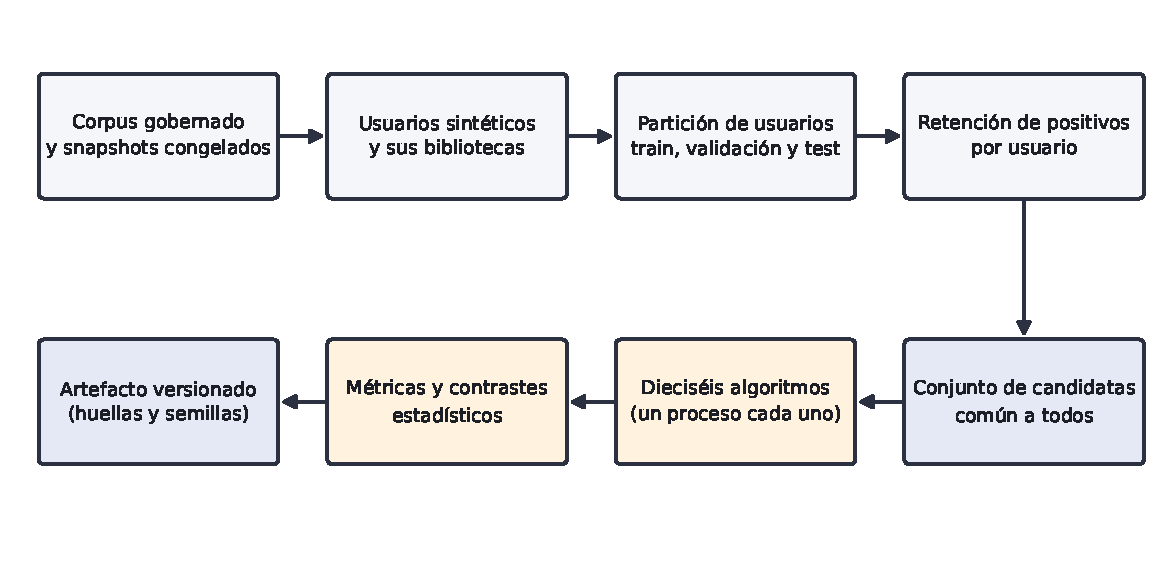
\includegraphics[width=0.9\textwidth]{figures/pipeline-evaluacion.pdf}
    \caption{Tubería de la evaluación sin conexión, de los datos congelados al artefacto versionado.}
    \label{fig:pipeline-evaluacion}
\end{figure}

La aplicación \texttt{evaluation} separa cuatro responsabilidades. El cargador del
protocolo valida las claves, el tamaño de la rejilla y el consumo único de la prueba. El módulo
de particiones selecciona la obra relevante retenida y comprueba que entrenamiento, validación y prueba
sean conjuntos disjuntos y completos. El módulo de métricas calcula la precisión y la exhaustividad (P@K y R@K), la ganancia acumulada descontada
normalizada (nDCG@K) y la precisión media (MAP@K) con fórmulas escritas y probadas en el proyecto. Por último, el ejecutor orquesta los algoritmos
y escribe un artefacto en notación de objetos de JavaScript (JSON) con sus huellas y resultados.

Todas las variantes comparten el conjunto de candidatos, la semántica de exclusión y el DTO
versionado; el modelo de contenido que usan es el descrito en la
Sección~\ref{cap:algoritmos}. Las explicaciones no generan texto libre: devuelven una tabla
determinista de contribuciones por faceta, el valor del término de valoración y si se usó la
alternativa de respaldo. El parámetro \texttt{algorithm\_id} solo puede seleccionar identificadores de una
lista permitida, nunca una función o importación dinámica.

Este capítulo ha descrito cómo se diseñaron la plataforma, los algoritmos de recomendación y el
laboratorio que los compara. El capítulo siguiente describe su implementación.

    \chapter{Implementación y pruebas}\label{cap:implementacion}\label{ap:implementacion-detallada}

Este capítulo describe cómo se ha construido el sistema. Empieza por el entorno reproducible y
las versiones fijadas, sigue con la adquisición y el gobierno de los datos, con el backend y con
el frontend; termina con las pruebas, la verificación y el despliegue. Incluye extractos de
código representativos, todos referenciados en el texto.

\section{Entorno reproducible y dependencias}\label{sec:impl-entorno}\label{sec:datos-dependencias}

El entorno de desarrollo y de pruebas se orquesta con Docker Compose, tal como describe la
Sección~\ref{sec:dis-arquitectura}. Las dependencias se fijan a versión exacta, con
\texttt{uv} para Python y \texttt{pnpm} para Node. Sus ficheros de bloqueo se congelan en las
construcciones. Las imágenes base se fijan por resumen criptográfico. La
Tabla~\ref{tab:stack} recoge las versiones principales.

\begin{table}[htp]
\centering
\begin{tabularx}{\textwidth}{ | L{0.24\textwidth} | C{0.18\textwidth} | Y | }
    \hline
    \textbf{Componente} & \textbf{Versión} & \textbf{Papel} \\
    \hline
    Python & 3.13.7 & Lenguaje del backend y de los guiones de datos. \\
    \hline
    Django & 5.2.17 LTS & Dominio, autenticación, ORM, sesiones y migraciones. \\
    \hline
    Django REST Framework & 3.18.0 & Serialización, permisos y API. \\
    \hline
    PostgreSQL & 18.6 & Base de datos de aplicación y de pruebas de integración. \\
    \hline
    psycopg & 3.3.5 & Controlador de PostgreSQL. \\
    \hline
    Node.js & 24.13.0 & Ejecución del frontend. \\
    \hline
    Next.js & 16.3.4 & Renderizado en el servidor, rutas y metadatos. \\
    \hline
    React & 19.2.7 & Modelo de componentes. \\
    \hline
    TypeScript & 6.0.3 & Tipado estricto del frontend. \\
    \hline
    Tailwind CSS & 4.3.3 & Tokens de diseño y maquetación adaptable. \\
    \hline
\end{tabularx}
\caption{Versiones principales del entorno reproducible.}
\label{tab:stack}
\end{table}

Toda dependencia directa nueva o cambio de versión pasa por un gate: aprobación humana
explícita, verificación de la ficha oficial del repositorio de paquetes, fijación a versión
exacta con su árbol transitivo en el fichero de bloqueo, una fila en
\texttt{docs/verification/dependency-legitimacy.md}, una fila en el gate
\texttt{check-dependencies.ps1} y una entrada en el registro de agentes. En el sistema solo
se añadieron dos dependencias directas. La primera es \texttt{requests} en la versión 2.34.2,
para el importador de IGDB. La segunda es \texttt{gunicorn} en la versión 23.0.0, como
servidor de producción de la API tras una revisión de código. Ambas se verificaron contra la
ficha oficial del índice de paquetes de Python, con su licencia, su versión mínima de
intérprete y su fecha de publicación reales.

\section{Adquisición y gobierno de datos}\label{cap:datos}

Esta sección describe de dónde salen los datos del catálogo, bajo qué licencia se usan y qué
evidencia de procedencia se conserva. El sistema integra dos fuentes de datos de catálogo. La
primera es un corpus curado de ciento cincuenta juegos procedente de Wikidata, que actúa como
la referencia citable y estable. La segunda es el catálogo a escala real procedente de IGDB,
con más de trescientas mil obras. Las dos conviven en la base de datos, indexadas por su
fuente, pero la evaluación solo consume la vista gobernada y versionada. La
Figura~\ref{fig:flujo-catalogo} recoge el recorrido completo de los datos, de las fuentes al
laboratorio.

\begin{figure}[htp]
    \centering
    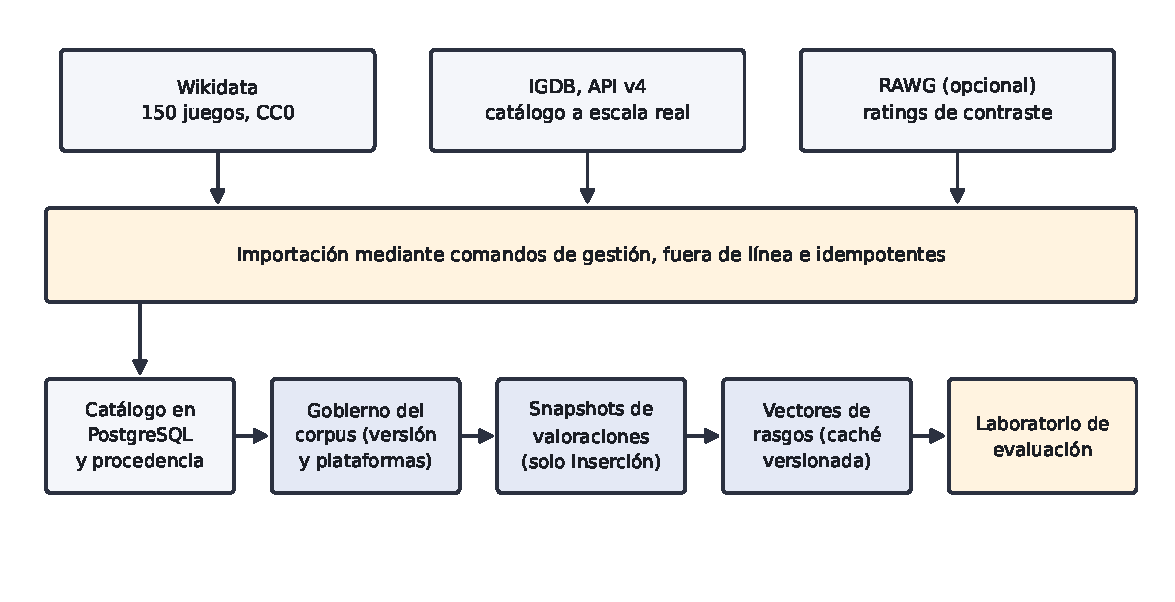
\includegraphics[width=0.9\textwidth]{figures/flujo-catalogo.pdf}
    \caption{Flujo de los datos del catálogo, desde las fuentes hasta el laboratorio de evaluación.}
    \label{fig:flujo-catalogo}
\end{figure}

\subsection{Fuentes: corpus de Wikidata y catálogo de IGDB}\label{sec:datos-wikidata}\label{sec:datos-igdb}

El corpus curado son ciento cincuenta juegos de datos estructurados de Wikidata,
publicados bajo la dedicación al dominio público \textit{Creative Commons Zero}
(CC0)~\cite{wikidata-licensing}. La adquisición se hace fuera de línea con un guion que
lanza una consulta filtrada por clase contra el punto de acceso del lenguaje de consulta SPARQL de Wikidata, resuelve
las subconsultas de plataforma de forma dinámica y valida la estructura y la cobertura por
época del resultado. El guion escribe el fichero \texttt{data/raw/wikidata-games.json} con su
huella SHA-256, más los manifiestos de catálogo y de recursos. El registro de decisión
ADR-003 y el documento \texttt{docs/verification/catalogue-freeze.md} conservan la consulta,
la fecha de corte en tiempo universal coordinado, la huella y la aprobación humana explícita
del corpus.

Los archivos multimedia se tratan por separado, porque no comparten la licencia de los datos
estructurados. De diecinueve archivos de Wikimedia Commons revisados uno a uno, diecisiete se
admitieron con crédito completo de autor, licencia y fuente. Los dos restantes se
sustituyeron por un marcador de reserva de primera parte~\cite{commons-reuse}. El identificador de Wikidata se
conserva solo como procedencia en \texttt{SourceRecord}, nunca como clave primaria, de modo
que la identidad del producto no queda acoplada a la fuente.

El catálogo a la escala de un producto real se construye con la API de
versión 4 de IGDB~\cite{igdb-api}. El requisito DATA-04 exige elegir la fuente mediante una
comparación documentada de cobertura, plataformas, licencia, atribución, cuotas, estabilidad
y coste. La Tabla~\ref{tab:data04} resume esa comparación, que se apoya en un sondeo
autenticado en vivo de la API ejecutado el 5 de septiembre de 2026 y en fuentes secundarias
para las otras dos opciones.

\begin{table}[htp]
\centering
\begin{tabularx}{\textwidth}{ | L{0.15\textwidth} | Y | Y | Y | }
    \hline
    \textbf{Eje} & \textbf{IGDB (elegida)} & \textbf{RAWG} & \textbf{Wikidata escalado} \\
    \hline
    Cobertura & 374.555 entradas totales, 312.418 juegos principales, medidos en vivo & Entre 350.000 y 500.000 declarados, fuente secundaria & Escasa y desigual para juegos \\
    \hline
    Plataformas & Entidad de primera clase, 220 filas & Metadatos de primera clase, fuente secundaria & Presentes pero inconsistentes \\
    \hline
    Licencia & \textit{Twitch Developer Services Agreement}, gratuita para uso comercial y no comercial & Nivel gratuito solo no comercial & CC0, la más limpia \\
    \hline
    Atribución & Estática y visible a IGDB.com & Obligatoria con enlace de vuelta en cada página & No requerida para datos CC0 \\
    \hline
    Cuotas & Sin cuota mensual; 4 peticiones por segundo & 20.000 peticiones al mes en el nivel gratuito & Sin cuota, sujeta a límites del punto de acceso \\
    \hline
    Estabilidad & API v4 estable desde 2020, respaldada por Twitch & Operador independiente, mayor riesgo & Muy estable como institución, datos de juegos volátiles \\
    \hline
    Coste & Cero & Cero dentro de la cuota & Cero \\
    \hline
\end{tabularx}
\caption{Comparación DATA-04 de fuentes para el catálogo a escala real.}
\label{tab:data04}
\end{table}

De la comparación se desprende la elección de IGDB, la única opción que combina cobertura
real, modelado de género y plataforma de primera clase, ausencia de cuota mensual y coste
cero, a cambio de una obligación de atribución continua. La frontera de categoría es
\texttt{game\_type = 0}, es decir, solo juegos principales; el contenido descargable, las
expansiones, los paquetes y los ports quedan excluidos del catálogo primario. Las portadas se
sirven por enlace directo al servidor de imágenes de IGDB, no se replican, con el marcador de
reserva de primera parte como alternativa cuando una portada falta o falla. La
regla de caché y redistribución se apoya en el texto de la propia documentación de la API,
que prefiere que el integrador almacene y sirva los datos a sus usuarios finales, texto que
se registra literalmente en el repositorio como la autorización escrita que contempla el
acuerdo general~\cite{twitch-dsa}. El corpus de Wikidata y su regla de no consultar
proveedores en tiempo de petición se conservan sin cambios; la importación de IGDB es aditiva
y se ejecuta solo desde un comando de gestión fuera de línea.

\subsection{Congelación y gobierno del corpus}\label{sec:datos-congelacion}

Una revisión humana fila a fila no es posible con cientos de miles de obras, ni es el modelo
legal correcto para las portadas de IGDB. El documento
\texttt{docs/verification/igdb-catalogue-freeze.md} congela en su lugar tres artefactos: una
huella de contenido, que es un SHA-256 sobre los pares de identificador de origen y huella
normalizada de cada registro de procedencia de IGDB, ordenados por identificador numérico;
una cobertura agregada, con el total de obras primarias, la distribución de géneros, las
plataformas más frecuentes, el histograma de año de lanzamiento y el reparto entre portada
presente y de reserva; y un manifiesto de revisión muestreada determinista de trescientos
registros, tomando uno de cada mil cuarenta y uno por orden de identificador, con datos
suficientes para una comprobación humana puntual. La Tabla~\ref{tab:freeze} recoge los
valores medidos en la carga de la base de datos de desarrollo persistente y actualizados
durante el gobierno del corpus, el 7 de septiembre de 2026.

\begin{table}[htp]
\centering
\begin{tabularx}{\textwidth}{ | L{0.60\textwidth} | Y | }
    \hline
    \textbf{Campo} & \textbf{Valor} \\
    \hline
    Obras primarias de IGDB importadas & 312.560 \\
    \hline
    Corpus de Wikidata conservado & 150 \\
    \hline
    Total de obras en el catálogo & 312.710 \\
    \hline
    Géneros & 23 \\
    \hline
    Plataformas (Wikidata e IGDB reconciliadas) & 288 \\
    \hline
    Portadas presentes / de reserva & 268.679 / 43.804 \\
    \hline
    Fecha de primer lanzamiento poblada & aproximadamente el 75\% de las filas \\
    \hline
    Obras con valoración de usuarios de IGDB & 27.014 (13,9330\% del corpus gobernado) \\
    \hline
    Cobertura de \texttt{total\_rating} & 15,8197\% del corpus gobernado \\
    \hline
    Huella de contenido (SHA-256) & \texttt{ff3d67525c92\ldots} \\
    \hline
\end{tabularx}
\caption{Evidencia agregada de congelación de la importación de IGDB.}
\label{tab:freeze}
\end{table}

La importación se probó además sobre una base de datos desechable, donde sobrevivió a una
interrupción abrupta tras dos lotes confirmados y reanudó hasta completar sin duplicados ni
huecos. Una segunda pasada completa sobre la base ya poblada convergió de forma idempotente,
con la única diferencia de dos juegos primarios que IGDB añadió en vivo entre las dos
pasadas. La versión inmutable reutilizable de la base cargada, de noventa y tres megabytes, no se
versiona en el repositorio por decisión de ADR-006; se conserva fuera de él como vía de
restauración rápida.

El laboratorio de evaluación añadió una frontera sobre este catálogo. El comando
\texttt{govern\_corpus} aplica las reglas D-03 de forma reversible: conserva las obras
fuente, pero marca como gobernadas las que son obras principales, tienen fecha de lanzamiento,
al menos un género y al menos una plataforma de la lista permitida de 39 plataformas. La valoración no es un criterio de
exclusión. La ejecución documentada el 7 de septiembre dejó 193.885 obras gobernadas y una versión de corpus
\texttt{2026.09.1}; el checksum, el diccionario, el informe de calidad y la muestra
determinista se conservan en \texttt{docs/verification/corpus-governance-freeze.md}. La
Tabla~\ref{tab:freeze} y las cifras de este párrafo corresponden a esa versión. El 9 de septiembre se
congeló la versión \texttt{2026.09.2}, con corte temporal en esa fecha: el catálogo visible no contiene
obras posteriores al corte, sin fecha ni contenido descargable y deja \textbf{190.479 obras
gobernadas}. Es la versión con la que trabajan el laboratorio de evaluación y los resultados del
Capítulo~\ref{cap:resultados} y su evidencia está en
\texttt{docs/verification/corpus-governance-2026.09.2.json}.

\subsection{Valoraciones externas y aislamiento de la evaluación}\label{sec:datos-ratings}

Durante la reimportación de IGDB se añadieron los campos \texttt{rating},
\texttt{rating\_count} y \texttt{total\_rating\_count}, además del resumen y los alias
alternativos. El campo \texttt{rating} representa la valoración de usuarios de IGDB en una
escala de 0 a 100; \texttt{total\_rating} representa la valoración agregada disponible en
IGDB. Son señales distintas y por eso se almacenan con nombres distintos. En el corte de
\texttt{2026.09.1}, la cobertura de ambos campos sobre las obras gobernadas es la que recoge
la Tabla~\ref{tab:freeze}.

El comando \texttt{snapshot\_corpus\_ratings} copia las valoraciones externas a
\texttt{CorpusRatingSnapshot} con una operación insert-only asociada a una
\texttt{corpus\_version}. Una reimportación puede actualizar los campos vivos que usa la
interfaz y producir una versión posterior, pero no modifica la versión inmutable ya
utilizada por el laboratorio. Esta separación es la condición que permite repetir una
comparación y explicar qué datos recibió.

Como fuente secundaria se probó RAWG en una ejecución acotada a 10.000 obras seleccionadas
por \texttt{rating\_count} de IGDB. La reconciliación fue determinista: primero se intentó
el slug exacto y después el título normalizado junto con el año de lanzamiento. No se aplicó
emparejamiento difuso; las filas no emparejadas se descartaron y se contabilizaron. El resultado
fue de 8.575 emparejamientos y 1.425 descartes, con 8.575 versiones inmutables de RAWG insertadas. La
cobertura nueva fue cero porque las obras seleccionadas ya tenían valoración de IGDB. RAWG se
documenta, por tanto, como contraste de procedencia, no como una fuente que haya ampliado
la cobertura del corpus.

La valoración mostrada en la ficha es una decisión de producto diferente. Puede mezclar,
con pesos limitados por la cantidad de observaciones, la valoración externa y las valoraciones
locales de las personas usuarias. El laboratorio no lee esa mezcla derivada ni el
valor mutable de \texttt{GameWork}: utiliza las versiones inmutables de la versión fijada. Esta
distinción evita que una nueva valoración de una cuenta o una reimportación cambie
retroactivamente un resultado académico.

\section{Backend}\label{sec:impl-backend}

\subsection{Comandos de gestión y del laboratorio}\label{sec:impl-comandos}

Toda tarea de datos es un comando de gestión de Django, ejecutable fuera de la petición HTTP e
idempotente. El importador de Wikidata, \texttt{import\_catalogue}, carga el corpus curado
de Wikidata. El importador de IGDB, \texttt{import\_igdb\_catalogue}, recorre la API por
lotes con un cursor de identificador reanudable: cada lote se confirma dentro de una
transacción que también escribe el cursor. Un disparador de base de datos impide que ese
cursor retroceda, de modo que una ejecución interrumpida siempre reanuda hacia delante desde
el progreso real. La cadena de arranque del despliegue encadena la migración y la importación del
catálogo, como describe la Sección~\ref{cap:despliegue}.

La gobernanza y las valoraciones externas de la Sección~\ref{cap:datos} se ejecutan con
\texttt{govern\_corpus}, \texttt{snapshot\_corpus\_ratings} y \texttt{enrich\_rawg\_ratings}, que
trabaja por lotes con \textit{backoff} ante respuestas transitorias.
\texttt{backfill\_game\_aliases} reconstruye los alias normalizados para que la búsqueda sea útil
sobre el catálogo real.

El protocolo se carga desde \texttt{docs/methodology/protocol.json}. Los módulos de la
aplicación \texttt{evaluation} que describe la Sección~\ref{sec:dis-laboratorio} se
implementan con funciones deliberadamente pequeñas y explícitas.
\texttt{evaluation/protocol.py} rechaza una rejilla con más de 31 configuraciones y distingue
un protocolo todavía no consumido de una prueba ya ejecutada. \texttt{evaluation/metrics.py} no
delega la definición de P@K, R@K, nDCG@K o MAP@K en una librería externa.
\texttt{evaluation/splits.py} deriva la semilla del protocolo y del usuario, para que el orden
de las filas en la base de datos no altere la obra retenida.

\subsection{Vistas, búsqueda y filtrado}\label{sec:impl-vistas}\label{sec:impl-busqueda}

La configuración de DRF fija la autenticación por sesión como única clase de autenticación,
de modo que no queda habilitada ninguna vía de autenticación básica sin límite de ritmo. Los
límites de ritmo de las vistas anónimas de mayor coste son: cinco registros
por hora, diez intentos de acceso por minuto, treinta consultas de perfil por minuto
y ciento veinte búsquedas de catálogo por minuto. El número de proxies de confianza se lee de
una variable de entorno, con valor cero en local, para que el límite de ritmo por dirección
se agrupe correctamente detrás del proxy del mismo origen.

La búsqueda del catálogo es tolerante: primero coincidencia exacta, después por prefijo y por
último por similitud de trigramas para erratas pequeñas, siempre sobre el índice de alias
normalizados y sin ninguna llamada externa. Sobre ese resultado se cruzan los filtros de
plataforma, género, año y nota mínima. Una lista fija de claves de ordenación se traduce a un
\texttt{order\_by} determinista con desempate por identificador canónico. El texto de
ordenación que envía el cliente nunca se interpola: una clave desconocida produce un error
acotado antes de tocar el ORM. El Extracto de código~\ref{cod:sort} muestra esa lista de
ordenaciones permitidas.

\begin{lstlisting}[language=Python, caption={Lista fija de ordenaciones del catálogo, con desempate por identificador canónico (\texttt{apps/api/catalogue/search.py}).}, label={cod:sort}, captionpos=b]
# Cada clave resuelve a una tupla de argumentos de order_by que SIEMPRE
# termina en canonical_slug, de modo que todo orden es total y estable
# entre llamadas. Nada derivado de la entrada del cliente llega a este
# diccionario: una clave no reconocida lanza un error antes de construir
# la consulta.
SORT_ORDERS = {
    "title_asc": ("original_title", "canonical_slug"),
    "title_desc": ("-original_title", "canonical_slug"),
    "release_newest": (F("first_release_date").desc(nulls_last=True), "canonical_slug"),
    "release_oldest": (F("first_release_date").asc(nulls_last=True), "canonical_slug"),
    "rating_desc": (F("total_rating").desc(nulls_last=True), "canonical_slug"),
}
\end{lstlisting}

\subsection{Recomendadores en la aplicación}\label{sec:impl-heuristico}

La aplicación publica tres variantes del laboratorio (Sección~\ref{sec:alg-publicadas}), cada una
servida por su proceso trabajador. Además, el método de referencia \texttt{rank\_random\_v1} es el suelo de
comparación. Selecciona con
\texttt{random.Random(seed)} sobre los candidatos gobernados que no aparecen en la biblioteca
de la persona usuaria. Ordenar previamente los identificadores y guardar una huella de la
semilla, los candidatos y el resultado hace que la misma entrada produzca exactamente la
misma clasificación.

El modelo de contenido que usan los algoritmos, descrito en la
Sección~\ref{cap:algoritmos}, se apoya en \texttt{WorkFeatureVector}, una caché versionada y
no un modelo entrenado, que \texttt{rebuild\_feature\_vectors} rellena de forma idempotente. El
perfil de usuario se construye con los pesos de actividad descritos a continuación y la
valoración se mantiene fuera del vector para poder estudiarla como una señal independiente.

\begin{samepage}
Cada entrada de biblioteca aporta un peso de actividad a las etiquetas curadas de su obra,
según la fórmula del Extracto de código~\ref{cod:heuristico}. Un refactor posterior extrajo ese
cálculo al módulo \texttt{apps/api/recommendations/\_weights.py}, para que las variantes de
contenido y la construcción del perfil reutilicen una única definición en lugar de copiarla. La
contribución de la valoración no es lineal, como explica la Sección~\ref{cap:algoritmos}; sin
actividad suficiente, las variantes aplican sus reglas declaradas de arranque en frío.

\begin{lstlisting}[language=Python, basicstyle=\small\ttfamily, caption={Cálculo del peso de actividad de una entrada de biblioteca.}, label={cod:heuristico}, captionpos=b]
# Pesos compartidos por los perfiles de contenido.
# Una obra abandonada no aporta evidencia positiva.
_STATUS_WEIGHTS = {
    "completed": 3.0,
    "playing": 2.0,
    "pending": 1.0,
    "abandoned": 0.0,
}

# La intensidad crece de forma no lineal con la valoracion.
_RATING_DIVISOR = 10
RATING_INTENSITY_POWER = 2.0

def _rating_intensity(rating_half_steps):
    if rating_half_steps is None:
        return 0.0
    normalised = max(
        0.0,
        min(1.0, rating_half_steps / _RATING_DIVISOR),
    )
    return normalised ** RATING_INTENSITY_POWER

def _entry_weight(status, rating_half_steps):
    status_weight = _STATUS_WEIGHTS.get(status or "", 0.0)
    return status_weight + _rating_intensity(rating_half_steps)
\end{lstlisting}
\end{samepage}

\clearpage
\section{Frontend}\label{sec:impl-frontend}\label{sec:impl-rutas}\label{sec:impl-i18n}\label{sec:impl-proxy}

\begin{samepage}
La parte cliente usa el enrutador de aplicación de Next.js, con un segmento de idioma en la raíz de
la ruta. Las rutas del sistema son la página de inicio, el catálogo, el detalle de un
juego, la colección, las amistades, el perfil propio, el perfil de un amigo, las fuentes, el acceso, el registro y las
recomendaciones. Los componentes reutilizables son los que fija el contrato de diseño de la
Sección~\ref{sec:dis-ui}, además del armazón de la aplicación con su barra de navegación. Las páginas de solo lectura se renderizan en el servidor; los controles de biblioteca
son componentes de cliente que llaman a la API del mismo origen. Las
Figuras~\ref{fig:catalogo} y~\ref{fig:coleccion} muestran el catálogo con sus filtros y la
colección de la persona usuaria; todas las capturas de esta sección son del propio proyecto.
\end{samepage}

\begin{figure}[H]
    \centering
    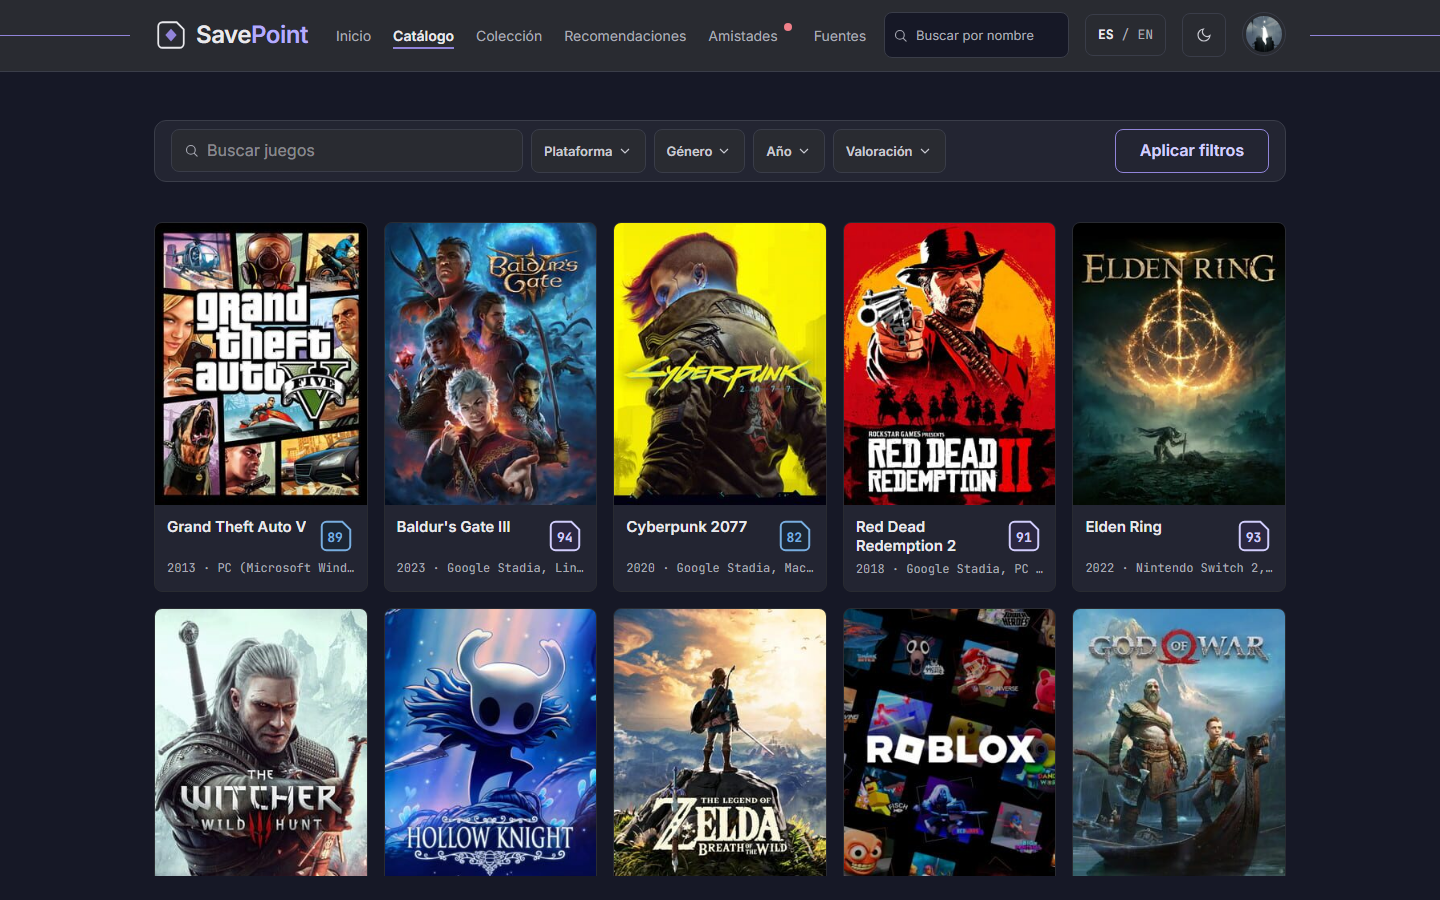
\includegraphics[width=0.85\textwidth]{figures/02-catalogo-oscuro.png}
    \caption{Catálogo con tema oscuro, búsqueda y filtros por plataforma, género, año y valoración.}
    \label{fig:catalogo}
\end{figure}

\begin{figure}[H]
    \centering
    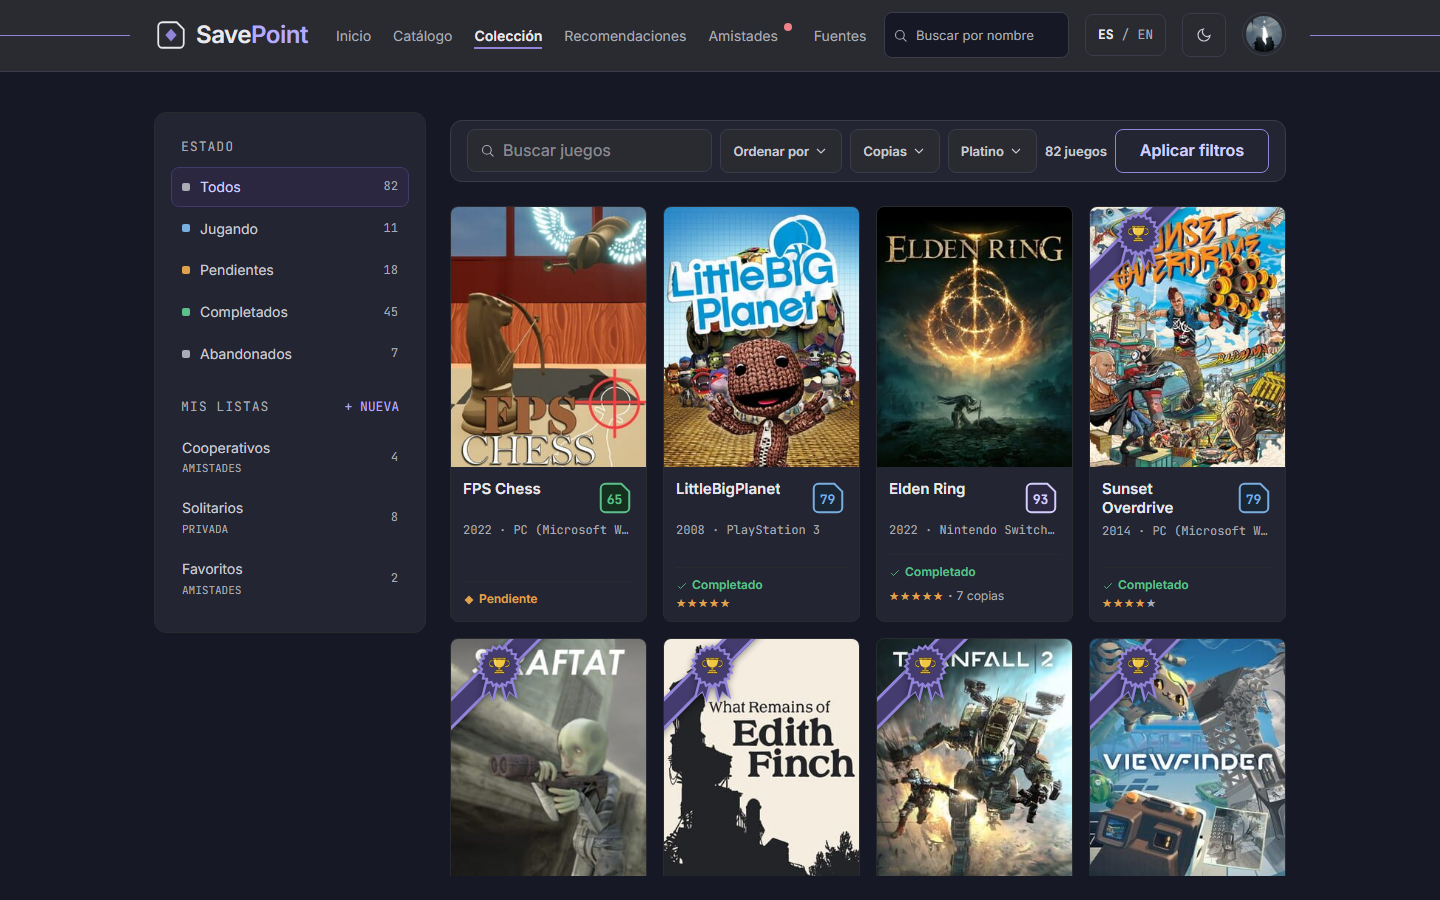
\includegraphics[width=0.85\textwidth]{figures/05-coleccion-oscuro.png}
    \caption{Colección de la persona usuaria con tema oscuro, con el estado y la valoración de cada juego.}
    \label{fig:coleccion}
\end{figure}

La interfaz está disponible en español y en inglés. Los textos viven en diccionarios por
idioma. Una prueba de paridad falla si una clave existe en un idioma pero no en el otro, de
modo que ninguna cadena queda sin traducir.

La reescritura del lado del servidor que describe la Sección~\ref{sec:dis-sesion} reenvía las
rutas bajo \texttt{/api/} y la ruta de chequeo de salud hacia el backend, con el destino tomado
de una variable de entorno visible únicamente en el servidor. El Extracto de
código~\ref{cod:proxy} la muestra.

\begin{lstlisting}[language=javascript, caption={Reescritura del mismo origen hacia el backend (\texttt{apps/web/next.config.ts}).}, label={cod:proxy}, captionpos=b]
// El navegador solo habla con este origen de Next.js: las cookies de
// sesion y CSRF que fija Django siguen siendo del mismo origen y no hace
// falta ninguna configuracion de CORS con credenciales. API_PROXY_TARGET
// solo existe en el entorno de servidor, nunca como variable NEXT_PUBLIC_.
async rewrites() {
  return [
    { source: "/api/:path*", destination: `${API_PROXY_TARGET}/api/:path*/` },
    { source: "/health/", destination: `${API_PROXY_TARGET}/health/` },
  ];
}
\end{lstlisting}

Las Figuras~\ref{fig:recomendaciones-estanterias}
y~\ref{fig:recomendaciones-detallada} muestran las dos vistas de recomendaciones disponibles
en el proyecto, junto a la portada ya presentada en la Figura~\ref{fig:ui-claro}; son capturas
de interfaz, no evidencia de calidad de clasificación ni de resultados experimentales.

\begin{figure}[H]
\centering
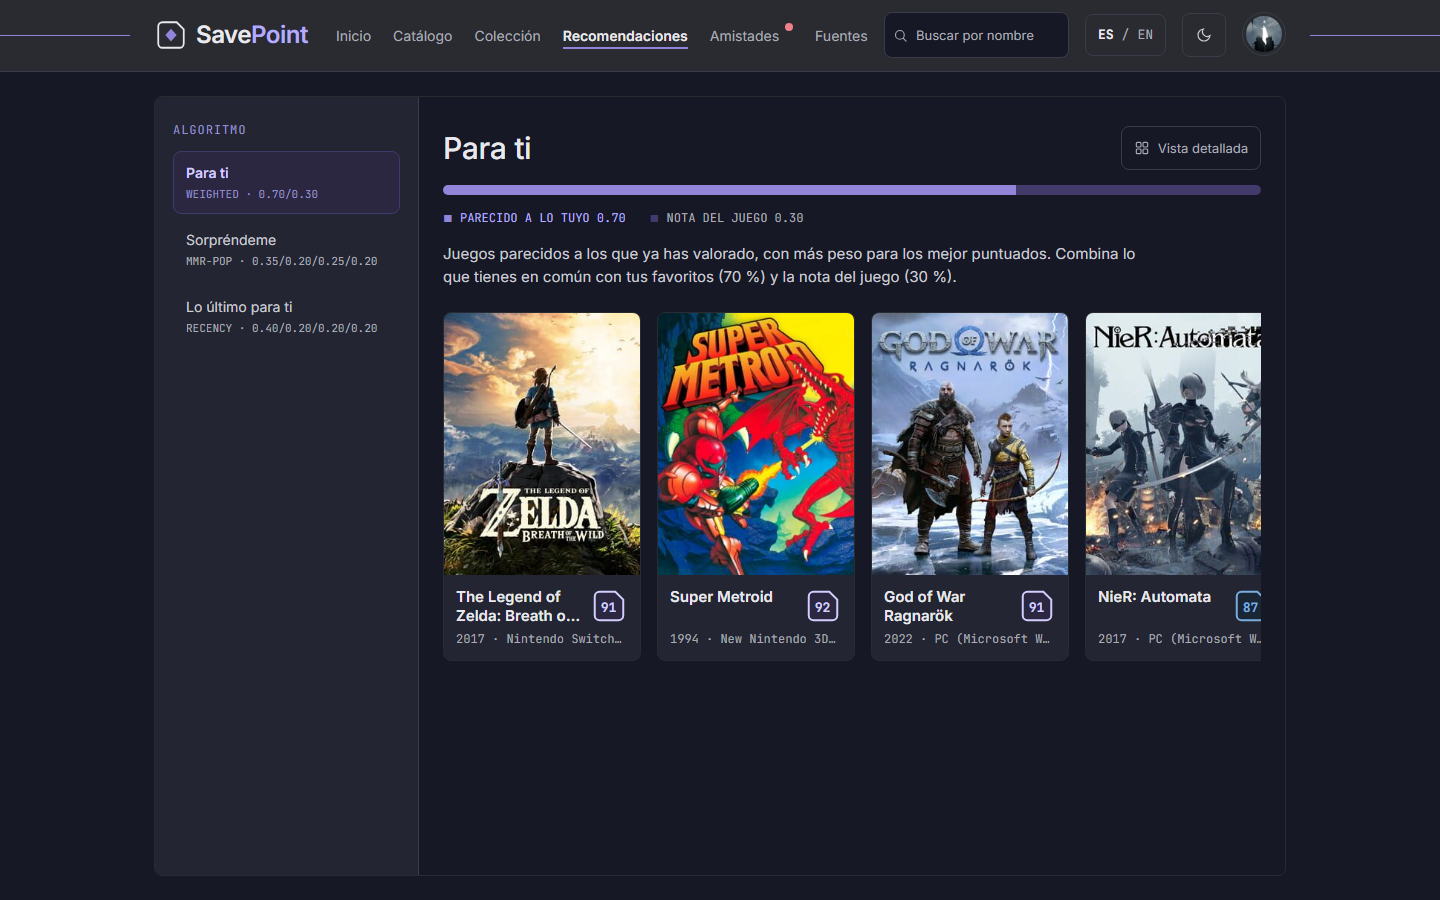
\includegraphics[width=0.82\textwidth]{figures/06-recomendaciones-estanterias-oscuro.png}
\caption{Vista de recomendaciones organizada por estanterías, con tema oscuro.}
\label{fig:recomendaciones-estanterias}
\end{figure}

\begin{figure}[H]
\centering
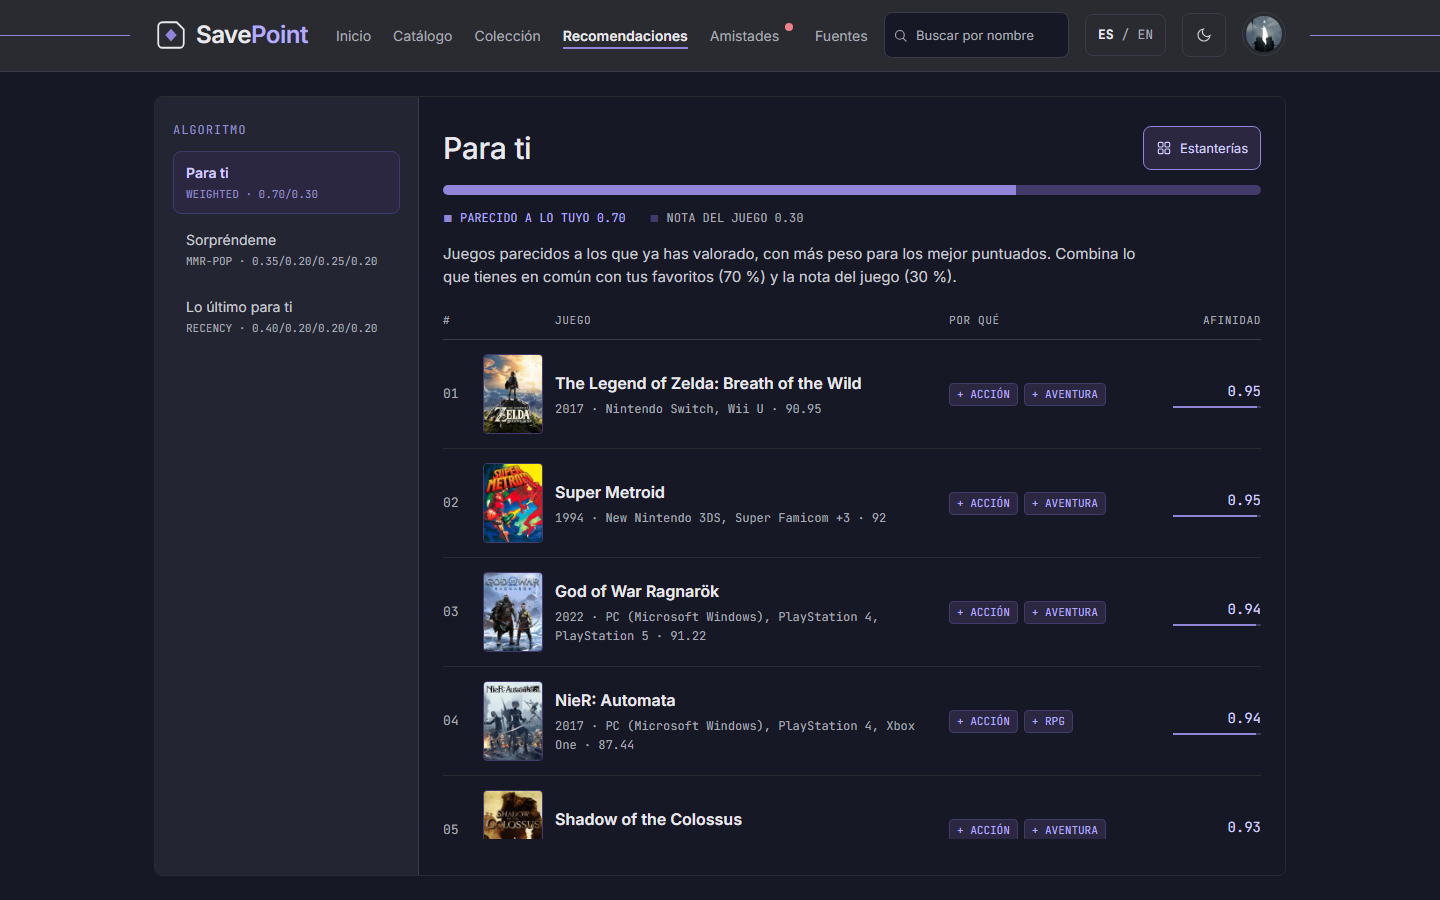
\includegraphics[width=0.82\textwidth]{figures/07-recomendaciones-detallada-oscuro.png}
\caption{Vista detallada de recomendaciones, con las señales de afinidad y tema oscuro.}
\label{fig:recomendaciones-detallada}
\end{figure}

El módulo social y de personalización se apoya en tres pantallas. La página de amistades
(Figura~\ref{fig:amistades}) reúne en tres columnas la búsqueda por nombre de usuario exacto
y la lista de amistades, el perfil de la persona elegida, con sus favoritos y un resumen de
su colección y las notificaciones de solicitudes y de recomendaciones, que pueden aceptarse,
rechazarse o responderse. La página de perfil propio (Figura~\ref{fig:perfil}) organiza los
ajustes en cinco pestañas: cuenta, privacidad, preferencias, conexiones y seguridad. La
primera permite editar el nombre completo, la biografía, la foto, la portada y los favoritos
y cambiar una única vez el nombre de usuario. El acceso (Figura~\ref{fig:acceso})
y el registro (Figura~\ref{fig:registro}) son los únicos formularios abiertos a visitantes.

\begin{figure}[H]
\centering
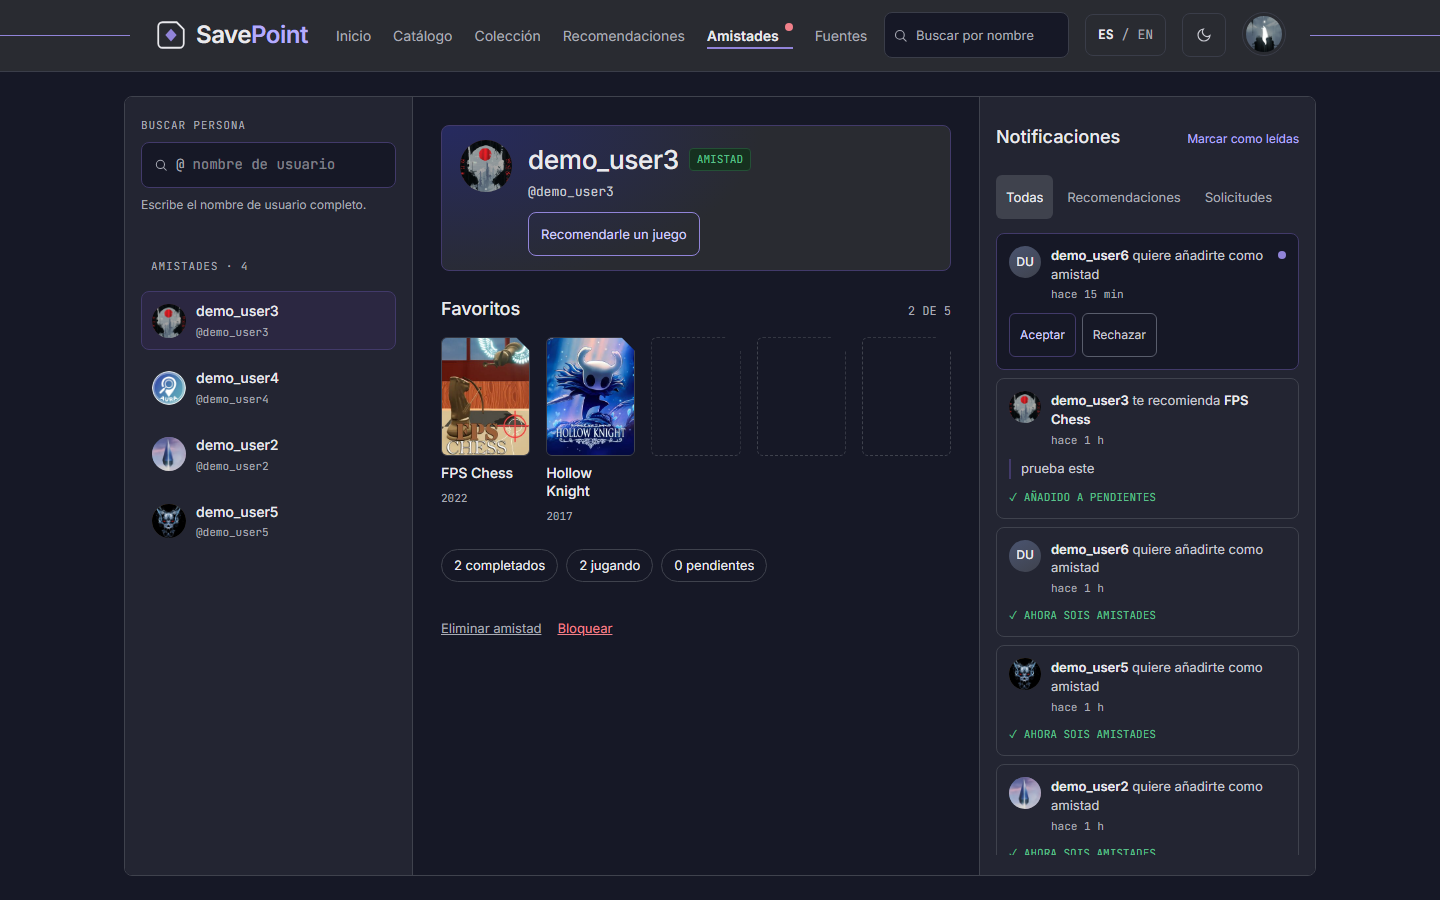
\includegraphics[width=0.85\textwidth]{figures/09-amistades-oscuro.png}
\caption{Página de amistades con tema oscuro: amistades, perfil de la persona elegida y notificaciones.}
\label{fig:amistades}
\end{figure}

\begin{figure}[H]
\centering
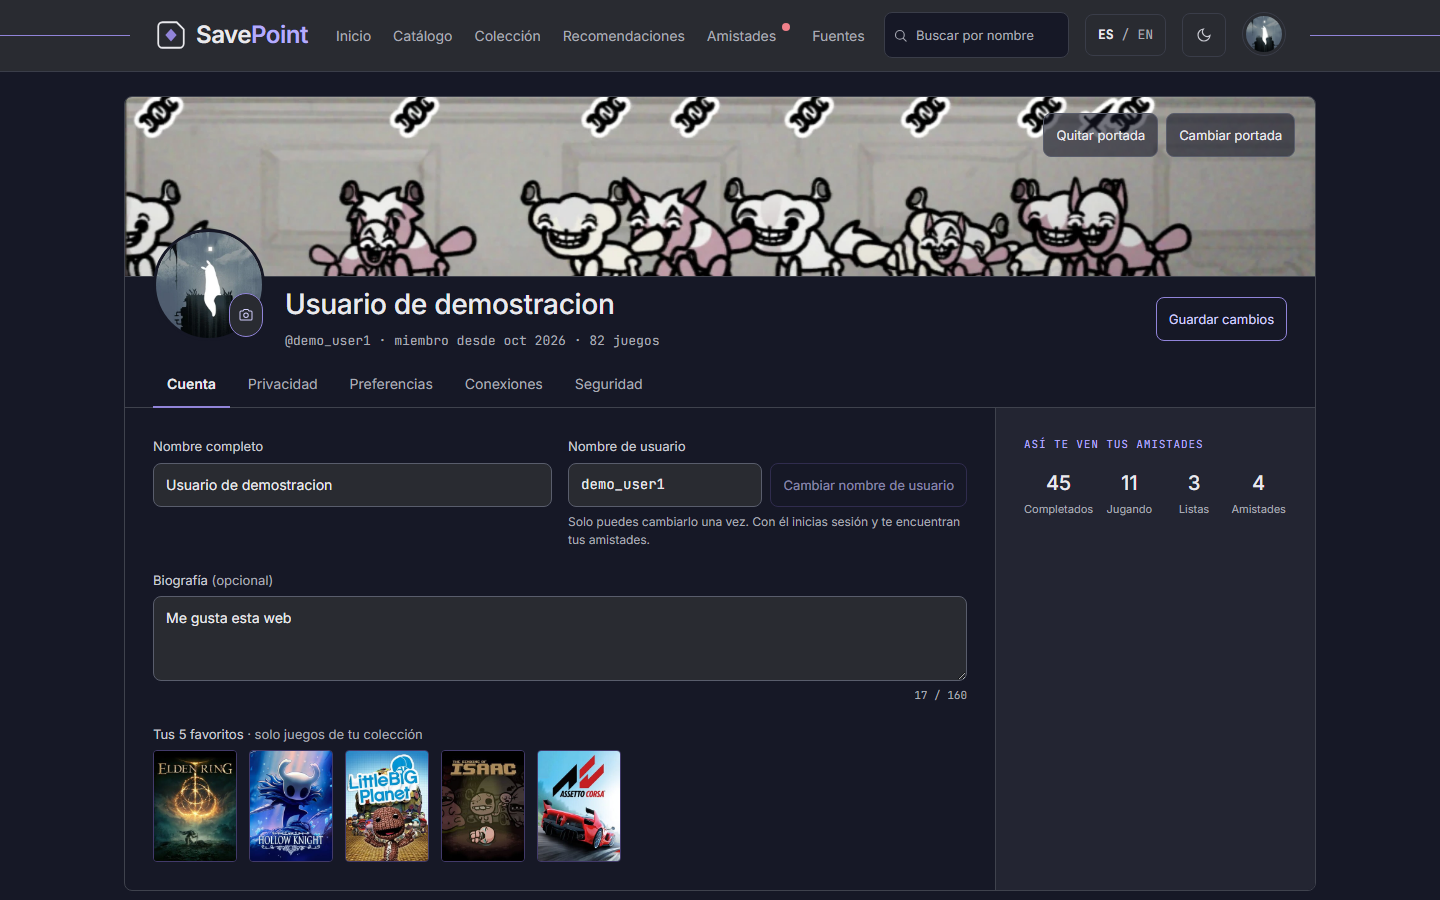
\includegraphics[width=0.85\textwidth]{figures/10-perfil-oscuro.png}
\caption{Perfil propio, pestaña de cuenta, con tema oscuro.}
\label{fig:perfil}
\end{figure}

\begin{figure}[H]
\centering
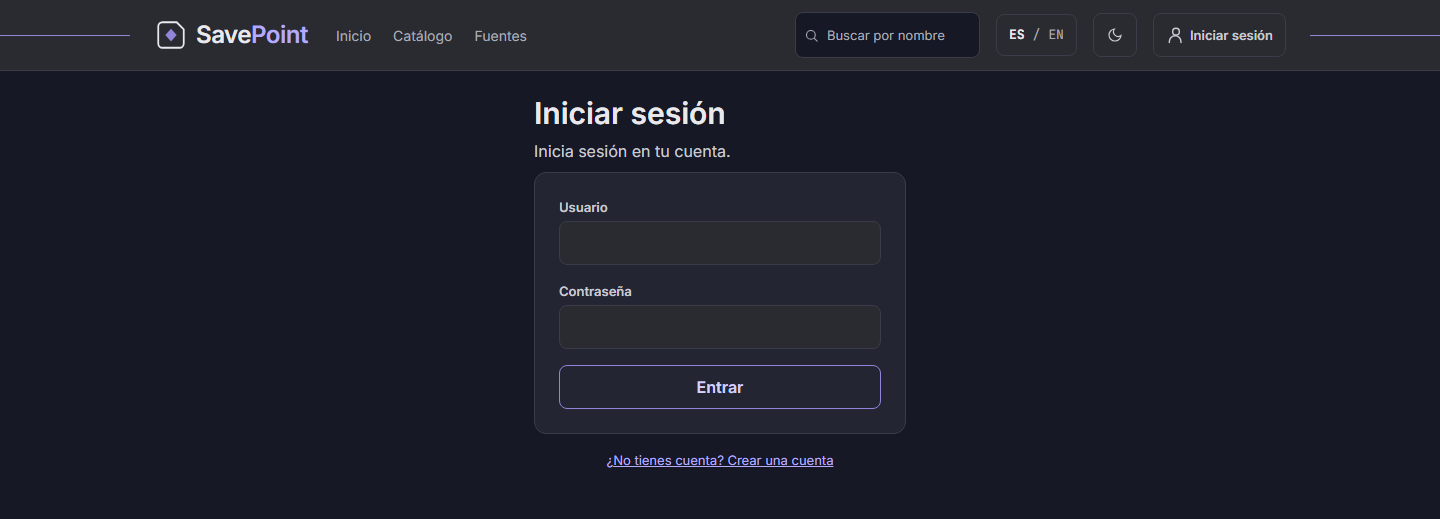
\includegraphics[width=0.85\textwidth]{figures/06-iniciar-sesion-oscuro.png}
\caption{Página de acceso con tema oscuro.}
\label{fig:acceso}
\end{figure}

\begin{figure}[H]
\centering
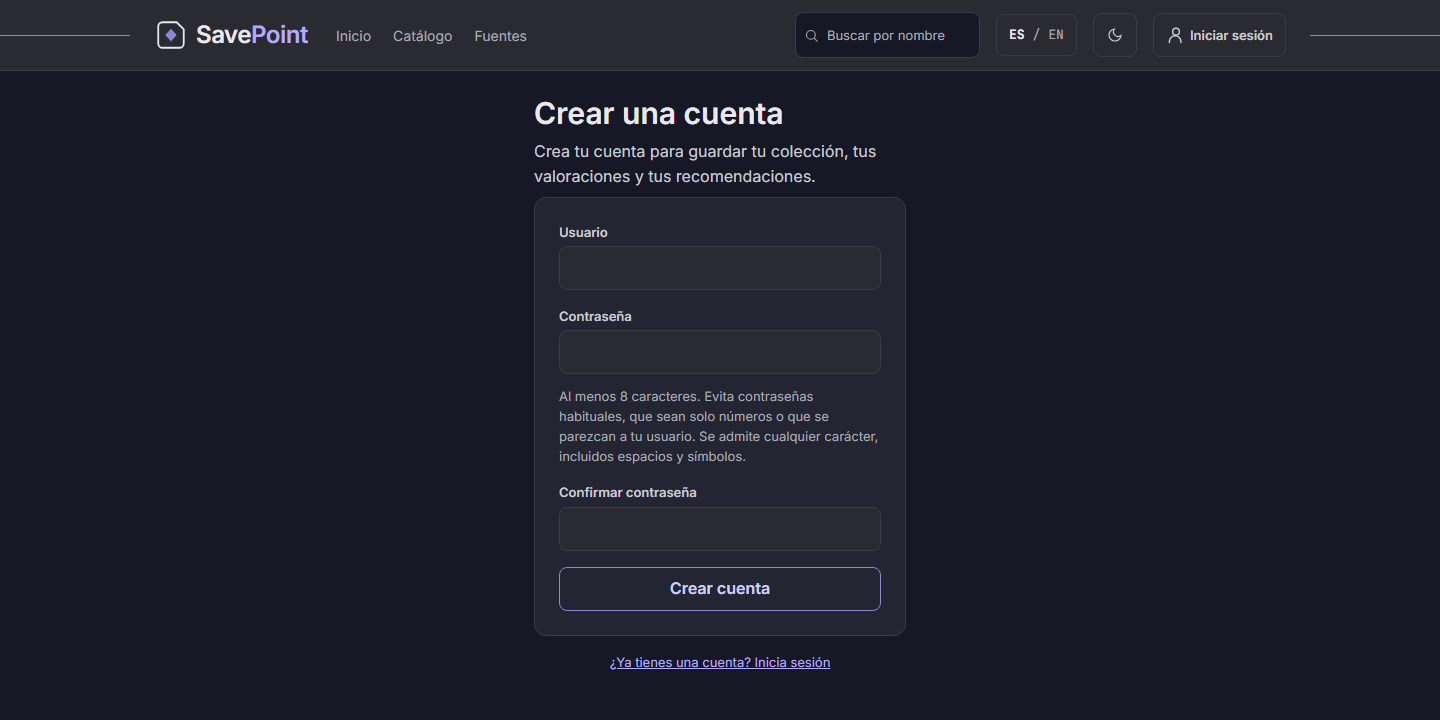
\includegraphics[width=0.85\textwidth]{figures/07-registro-oscuro.png}
\caption{Página de registro con tema oscuro.}
\label{fig:registro}
\end{figure}

\section{Pruebas y verificación}\label{cap:pruebas}\label{sec:pru-estrategia}

La verificación combina pruebas de backend contra PostgreSQL real (unitarias e integración en
una única suite \texttt{pytest}, sin separarlas en conteos independientes), pruebas de
frontend con Vitest y un recorrido de navegador con Playwright que integra los casos de
accesibilidad mediante \texttt{axe}, sin un conteo aislado solo de accesibilidad. El cierre de
evidencia final, ejecutado el 14 de septiembre de 2026 y registrado en
\texttt{docs/verification/phase-07-launch-gate.md} y en \texttt{07-VERIFICATION.md}, deja como
última regresión completa 736 pruebas de backend, 70 de frontend y 56 de navegador, las tres
en verde y sin omitidas. Tras los cambios posteriores de interfaz, del módulo social y del despliegue, el 5 de octubre de 2026 se repitieron las suites de backend y de frontend: 788 pruebas de backend y 66 de frontend, todas en verde y sin omitidas (Tabla~\ref{tab:pru-resultados}). El recorrido de navegador no se repitió después de esos cambios. Las evidencias de seguridad, migraciones, privacidad, importación y
exportación se citan desde \texttt{docs/verification/}.

La estrategia combina cuatro niveles. Las pruebas unitarias y de integración del backend se
ejecutan con \texttt{pytest} contra una instancia real de PostgreSQL 18.6, sin sustituirla
por una base en memoria, porque el sistema depende de restricciones, transacciones y búsqueda
de trigramas que solo se comportan igual sobre el motor real. Las pruebas del frontend usan
\texttt{vitest} para la lógica y los componentes, con una prueba de paridad de claves de
traducción. Las pruebas de extremo a extremo (E2E) usan Playwright sobre un navegador real, con la
biblioteca \texttt{axe} para las comprobaciones automáticas de accesibilidad frente a las
Pautas de Accesibilidad para el Contenido Web (WCAG) 2.2~\cite{wcag22}. Por último, una
prueba de humo se ejecuta contra la URL pública desplegada y rechaza un despliegue con la
revisión equivocada, tráfico entre orígenes inesperado o peticiones fallidas.

Las comprobaciones de \texttt{axe} cubren el catálogo, el detalle, el registro, las
recomendaciones, la página de inicio, el acceso y las fuentes, en escritorio a 1280 por 800
píxeles y en móvil a 375 por 812 píxeles.

\subsection{Resultados finales y trazabilidad}\label{sec:pru-resultados}\label{sec:pru-trazabilidad}

La Tabla~\ref{tab:pru-resultados} recoge el resultado final de cada suite y la
Tabla~\ref{tab:pru-areas} reparte las pruebas de backend por área del código. Los recuentos salen del
informe de la propia ejecución del 5 de octubre de 2026, no de una estimación.

\begin{table}[htp]
\centering
\begin{tabularx}{\textwidth}{ | L{0.20\textwidth} | L{0.22\textwidth} | C{0.10\textwidth} | Y | C{0.17\textwidth} | }
    \hline
    \textbf{Suite} & \textbf{Herramienta} & \textbf{Pruebas} & \textbf{Resultado} & \textbf{Fecha} \\
    \hline
    Backend & \texttt{pytest} sobre PostgreSQL 18.6 & 788 & 788 correctas, 0 fallidas, 0 omitidas (146 s) & 5-10-2026 \\
    \hline
    Frontend & Vitest (12 ficheros) & 66 & 66 correctas, 0 fallidas & 5-10-2026 \\
    \hline
    Navegador & Playwright con \texttt{axe} & 56 & 56 correctas, 0 omitidas & 14-09-2026 \\
    \hline
\end{tabularx}
\caption{Resultado final de cada suite de pruebas. El recorrido de navegador no se ha repetido desde el rediseño de la interfaz.}
\label{tab:pru-resultados}
\end{table}

\begin{table}[htp]
\centering
\begin{tabularx}{\textwidth}{ | L{0.24\textwidth} | C{0.12\textwidth} | Y | }
    \hline
    \textbf{Área} & \textbf{Pruebas} & \textbf{Qué cubre} \\
    \hline
    Catálogo (\texttt{catalogue}) & 156 & Importación del catálogo, búsqueda, ficha con procedencia, versiones inmutables de valoraciones y popularidad. \\
    \hline
    Evaluación (\texttt{evaluation}) & 154 & Protocolo, particiones, métricas, ejecutor, población sintética y API del panel de investigación. \\
    \hline
    Biblioteca (\texttt{library}) & 140 & Estado, valoración, copias, listas, comentarios, popularidad y exportación. \\
    \hline
    Cuentas (\texttt{accounts}) & 134 & Registro, sesión, perfil, privacidad y cuentas de demostración. \\
    \hline
    Recomendaciones (\texttt{recommendations}) & 119 & Vectores, perfil de gusto, similitud, familias de algoritmos y recomendador por géneros. \\
    \hline
    Transversales (\texttt{tests}) & 82 & Amistades, visibilidad, mensajes, administración, seguridad y endurecimiento. \\
    \hline
    Auditoría (\texttt{audit}) & 3 & Registro de auditoría de solo anexado. \\
    \hline
    \textbf{Total} & \textbf{788} & \\
    \hline
\end{tabularx}
\caption{Pruebas de backend por área.}
\label{tab:pru-areas}
\end{table}

La Tabla~\ref{tab:pru-trazabilidad} relaciona cada caso de uso de la Tabla~\ref{tab:casos-uso} con los requisitos que cubre, los ficheros de
prueba que los verifican y el número de pruebas de cada uno; los
requisitos de datos y de evaluación, que verifican las suites de las áreas \texttt{catalogue} y
\texttt{evaluation}, se tratan en la Sección~\ref{sec:pru-datos}.

\begin{table}[htp]
\centering
\small
\begin{tabularx}{\textwidth}{ | C{0.17\textwidth} | C{0.13\textwidth} | Y | C{0.12\textwidth} | }
    \hline
    \textbf{Requisito} & \textbf{Caso de uso} & \textbf{Fichero de pruebas} & \textbf{Pruebas} \\
    \hline
    CAT-01 & CU-1 & \path{catalogue/tests/test_search.py} & 49 \\
    \hline
    CAT-02 & CU-3 & \path{catalogue/tests/test_search.py}, \path{lib/__tests__/catalogue-filters.test.ts} & 49, 11 \\
    \hline
    CAT-03 & CU-2 & \path{catalogue/tests/test_detail.py}, \path{catalogue/tests/test_sources.py} & 6, 2 \\
    \hline
    REC-02 & CU-4 & \path{library/tests/test_popularity.py} & 12 \\
    \hline
    AUTH-01 & CU-5, CU-6 & \path{accounts/tests/test_registration.py}, \path{accounts/tests/test_auth.py} & 17, 10 \\
    \hline
    LIB-01 & CU-7 & \path{library/tests/test_entry.py} & 18 \\
    \hline
    LIB-02 & CU-8 & \path{library/tests/test_rating.py} & 19 \\
    \hline
    INV-01, INV-02 & CU-9 & \path{library/tests/test_copies.py} & 25 \\
    \hline
    REC-10 & CU-10 & \path{recommendations/tests/test_genre_heuristic.py} & 29 \\
    \hline
    SOCIAL-03 & CU-11 & \path{tests/test_social.py} & 10 \\
    \hline
    SOCIAL-04 & CU-12 & \path{tests/test_social_visibility.py} & 12 \\
    \hline
    LIB-03, SOCIAL-04 & CU-13 & \path{library/tests/test_comments.py} & 8 \\
    \hline
    PROF-01 & CU-14 & \path{accounts/tests/test_profile.py}, \path{accounts/tests/test_profile_page.py} & 19, 13 \\
    \hline
    SOCIAL-05 & CU-15 & \path{tests/test_social_messages.py} & 6 \\
    \hline
\end{tabularx}
\caption{Relación entre requisitos, casos de uso y pruebas automatizadas del backend, salvo la fila de filtros, que incluye también una prueba del frontend.}
\label{tab:pru-trazabilidad}
\end{table}

Como ejemplo de caso de prueba concreto, la Tabla~\ref{tab:pru-cp1} describe la comprobación de que reintentar el
alta de una copia no crea un duplicado y la Tabla~\ref{tab:pru-cp2} la de que una persona sin permiso no puede
distinguir una colección privada de una que no existe. Ambas son pruebas automatizadas del repositorio y pasan en la
ejecución final de la Tabla~\ref{tab:pru-resultados}.

\begin{table}[htp]
\centering
\small
\begin{tabularx}{\textwidth}{ | L{0.22\textwidth} | Y | }
    \hline
    \textbf{Caso} & \textbf{CP-1: reintento idempotente del alta de una copia (INV-02)} \\
    \hline
    Objetivo & Un reenvío de la misma petición, por ejemplo por un doble clic o un fallo de red, no debe crear una copia duplicada. \\
    \hline
    Precondiciones & Una persona usuaria y una obra con una publicación. \\
    \hline
    Pasos & 1) Crear una copia física con la clave de idempotencia \texttt{replay-key}. 2) Repetir la misma operación con la misma clave. \\
    \hline
    Resultado esperado & La primera operación crea la copia; la segunda devuelve la misma copia sin crear otra; la persona tiene una sola copia. \\
    \hline
    Prueba automatizada & \path{library/tests/test_copies.py}, \texttt{test\_\allowbreak{}replaying\_\allowbreak{}idempotency\_\allowbreak{}key\_\allowbreak{}returns\_\allowbreak{}same\_\allowbreak{}copy\_\allowbreak{}not\_\allowbreak{}a\_\allowbreak{}duplicate}; la unicidad también se exige en la base de datos (\path{library/tests/test_schema.py}). \\
    \hline
    Resultado & Superada. \\
    \hline
\end{tabularx}
\caption{Caso de prueba CP-1.}
\label{tab:pru-cp1}
\end{table}

\begin{table}[htp]
\centering
\small
\begin{tabularx}{\textwidth}{ | L{0.22\textwidth} | Y | }
    \hline
    \textbf{Caso} & \textbf{CP-2: una colección ajena no revela su existencia (SOCIAL-04)} \\
    \hline
    Objetivo & Quien no es amistad del propietario, o no ha iniciado sesión, no debe poder distinguir una colección o una lista privadas de las de un usuario que no existe. \\
    \hline
    Precondiciones & Un propietario con una colección y una lista pública, una persona autenticada que no es su amistad y un visitante anónimo. \\
    \hline
    Pasos & Como visitante y como persona sin amistad: 1) pedir la lista del propietario; 2) pedir su colección; 3) pedir la colección de un alias inexistente. \\
    \hline
    Resultado esperado & Las tres peticiones responden 404 y la respuesta de la lista y de la colección del propietario es idéntica a la del alias inexistente. \\
    \hline
    Prueba automatizada & \path{tests/test_social_visibility.py}, \texttt{test\_\allowbreak{}anonymous\_\allowbreak{}and\_\allowbreak{}non\_\allowbreak{}friend\_\allowbreak{}get\_\allowbreak{}same\_\allowbreak{}404\_\allowbreak{}for\_\allowbreak{}direct\_\allowbreak{}collection\_\allowbreak{}and\_\allowbreak{}list}. \\
    \hline
    Resultado & Superada. \\
    \hline
\end{tabularx}
\caption{Caso de prueba CP-2.}
\label{tab:pru-cp2}
\end{table}

\subsection{Verificación de los datos y del laboratorio}\label{sec:pru-datos}

La verificación de los datos y del laboratorio se dividió en dos grupos. El primero comprobó que los datos y
sus contratos eran correctos: 70 pruebas del catálogo cubrieron la importación de campos de
valoración, las versiones inmutables de solo inserción y la reconciliación determinista de RAWG; 54 pruebas de
la aplicación \texttt{evaluation} cubrieron el cargador de protocolo, las particiones y las
métricas. El segundo comprobó las primitivas de recomendación: 48 pruebas cubrieron el
método de referencia aleatorio, el coseno, los vectores de contenido, el perfil de usuario, la caché
\texttt{WorkFeatureVector} y el cálculo del perfil de valoración por género.

Las propiedades relevantes se verificaron con casos pequeños y respuestas conocidas. El
método de referencia aleatorio devuelve el mismo orden para la misma semilla, no devuelve obras de la
biblioteca y no sale del corpus gobernado. La similitud coseno queda acotada entre cero y
uno, es exactamente uno para vectores iguales no nulos y vale cero para vectores ortogonales
o sin norma. Las métricas se comparan con cálculos manuales, mientras que la partición rechaza
conjuntos de entrenamiento, validación y prueba que no sean disjuntos y completos.

La prueba de datos a escala también dejó una evidencia reproducible. El enriquecimiento RAWG
se ejecutó en 18 lotes y una repetición de un lote ya procesado insertó cero versiones inmutables
adicionales. La huella de \texttt{GameWork.rating} permaneció idéntica antes y después, lo
que demuestra que el enriquecimiento no muta el valor vivo del catálogo. Esta evidencia
prueba integridad e idempotencia; no prueba que RAWG haya mejorado la calidad de las
recomendaciones.

Las tablas de precisión, recall, nDCG y MAP de la comparación completa, con las 16 variantes evaluadas, sus contrastes de significación estadística y sus amenazas a la validez, se presentan en el Capítulo~\ref{cap:resultados}.

\subsection{Gates de evidencia y verificación independiente}\label{sec:pru-gates}\label{sec:pru-verificacion-fase}

Además de las pruebas, el repositorio tiene gates deterministas que protegen la evidencia. El
gate \texttt{check-secrets.ps1} escanea el árbol de Git, los paquetes de construcción, las
capas de las imágenes y los registros capturados en busca de cadenas con forma de credencial
y se autoverifica primero contra señuelos sintéticos. El gate \texttt{check-evidence.ps1}
valida el registro de agentes descrito en la Sección~\ref{sec:met-ledger} y el gate
\texttt{check-dependencies.ps1} comprueba la lista permitida de dependencias de la
Sección~\ref{sec:impl-entorno}. Los gates \texttt{verify-igdb-*.ps1} comprueban el contenido del
registro de decisión de IGDB, la evidencia del sondeo y la ejecución de importación sobre una
base de datos fresca.

Cada incremento del sistema se sometió a la verificación independiente de su objetivo que
describe la Sección~\ref{sec:met-agentes}, que comprueba el código contra los criterios de
éxito en lugar de leer los resúmenes de plan. El recorrido vertical
inicial se verificó con cinco de cinco criterios de éxito, con dos elementos manuales de
accesibilidad aceptados como limitaciones nombradas: el reflujo al cuatrocientos por ciento
de zoom y una pasada con lector de pantalla. El catálogo a escala real, el rediseño de la
interfaz y los recomendadores se verificaron con cuatro de cuatro criterios. La Tabla~\ref{tab:criterios} resume esos criterios.

\begin{table}[htp]
\centering
\begin{tabularx}{\textwidth}{ | C{0.12\textwidth} | Y | C{0.19\textwidth} | }
    \hline
    \textbf{Criterio} & \textbf{Enunciado} & \textbf{Veredicto} \\
    \hline
    SC1 & Catálogo a escala real con fuente IGDB, con licencia, atribución y procedencia documentadas. & Verificado \\
    \hline
    SC2 & Ordenar y filtrar el catálogo por plataforma, género y otros metadatos. & Verificado \\
    \hline
    SC3 & La interfaz se lee como un producto de catalogación profesional. & Verificado \\
    \hline
    SC4 & Página de recomendaciones por géneros según la actividad propia, distinta de la recomendación de referencia por popularidad. & Verificado \\
    \hline
\end{tabularx}
\caption{Criterios de éxito verificados y su veredicto.}
\label{tab:criterios}
\end{table}

El criterio SC3, la calidad visual de producto, se cerró con la aprobación final. Empezó
como aprobación anticipada condicional, concedida sin acceso directo al entorno. Quedó
confirmada sin condiciones tras una revisión remota de dieciocho capturas del entorno local
que cubrían las cuatro superficies principales en escritorio y en móvil, ambos temas y una
segunda cuenta con colección vacía como prueba visual de independencia.

\subsection{Revisión de código}\label{sec:pru-revision}\label{sec:pru-post-cierre}\label{sec:pru-lectura}

Ya con el sistema completo, el revisor de código de la Sección~\ref{sec:met-agentes} examinó
todo el árbol con una postura adversarial de búsqueda de defectos.
La revisión encontró dieciséis hallazgos, cuya distribución por severidad recoge la
Tabla~\ref{tab:hallazgos}. Se autorizó aplicar la totalidad de los hallazgos, que se
corrigieron en cinco tandas confirmadas, cada una con las pruebas ejecutadas después.

\begin{table}[htp]
\centering
\begin{tabularx}{\textwidth}{ | L{0.25\textwidth} | C{0.18\textwidth} | Y | }
    \hline
    \textbf{Severidad} & \textbf{Hallazgos} & \textbf{Estado} \\
    \hline
    Crítica & 0 & Ninguno \\
    \hline
    Alta & 3 & Corregidos \\
    \hline
    Media & 6 & Corregidos \\
    \hline
    Baja & 7 & Corregidos \\
    \hline
    \textbf{Total} & \textbf{16} & \textbf{16 corregidos} \\
    \hline
\end{tabularx}
\caption{Hallazgos de la revisión de código de todo el repositorio.}
\label{tab:hallazgos}
\end{table}

Los tres hallazgos de severidad alta ilustran el valor de una revisión con contexto
independiente. El primero era que la configuración de DRF dejaba habilitada de forma
silenciosa la autenticación básica en todo punto de acceso autenticado, lo que abría una vía
de adivinación de contraseñas sin límite de ritmo y una ruta de cambio de estado exenta de la
protección contra falsificación de petición en sitios cruzados. El segundo era que una
reimportación troceada del catálogo de IGDB tras una pasada completa podía saltarse en
silencio un rango de identificadores ya recorrido y aun así declararse completa con una huella
nueva. El tercero era que el arranque de producción usaba el servidor de desarrollo de
Django, que su documentación desaconseja explícitamente. Los tres se corrigieron, el segundo
con un campo de esquema nuevo y una migración, el tercero con la incorporación del servidor
\texttt{gunicorn}.

La revisión también dejó constancia de las áreas sanas: ausencia de inyección de lenguaje de consulta estructurado (SQL), con
todo el uso del ORM parametrizado; validación minuciosa de las consultas del catálogo;
acotación de propiedad en todas las vistas de datos personales; escrituras transaccionales
con bloqueo de fila y restricciones de unicidad como guarda real de carreras; higiene de
secretos con redacción en registros y excepciones.

Tras la revisión de producto del proyecto, una tanda de correcciones se aplicó sobre la rama
principal. La página de inicio dejó de
mostrar una llamada a la acción de acceso redundante. El formulario de registro pasó a
devolver los incumplimientos concretos de la política de contraseñas en lugar de un mensaje
impreciso. La comparación del nombre de usuario en el acceso se hizo insensible a mayúsculas,
para casar con la comprobación de unicidad, que ya lo era. Se añadió un punto de acceso
pequeño, \texttt{GET /api/accounts/me/}, para que la barra de navegación pueda nombrar la
cuenta activa.

Las cifras anteriores respaldan afirmaciones acotadas. El sistema tiene una cobertura de
pruebas amplia sobre PostgreSQL real, una accesibilidad automática sólida aunque no
exhaustiva y una revisión de seguridad de todo el árbol con sus hallazgos corregidos. Esas
cifras no respaldan ninguna medida de rendimiento bajo carga, de recuperación ante desastre
ni de calidad de recomendación, que se mide aparte en el Capítulo~\ref{cap:resultados}. Los dos elementos manuales de accesibilidad del recorrido inicial siguen abiertos y
declarados como tales.

\section{Despliegue}\label{cap:despliegue}

La restricción de partida del despliegue público es la misma que ya fijó su diseño: coste
cero, sin introducir ninguna tarjeta de pago ni habilitar ningún recurso de facturación. La
Tabla~\ref{tab:topologia} recoge el contrato de cada superficie.

\begin{table}[H]
\centering
\begin{tabularx}{\textwidth}{ | L{0.21\textwidth} | L{0.19\textwidth} | Y | }
    \hline
    \textbf{Superficie} & \textbf{Servicio} & \textbf{Contrato} \\
    \hline
    Interfaz de navegador & Vercel Hobby & Construye el frontend Next.js; reenvía del lado del servidor las rutas de la API y de salud hacia Render. \\
    \hline
    API & Render Free & Construye la imagen de la API con el catálogo local congelado y expone la ruta de salud. \\
    \hline
    Base de datos & Neon Free & Proyecto \texttt{autumn-breeze-06234770}, rama \texttt{production}; suministra PostgreSQL a Render. \\
    \hline
    Cálculo & Proceso de Render & Un único proceso corto que la API lanza bajo demanda, vacía la cola de trabajos de recomendación y termina. \\
    \hline
\end{tabularx}
\caption{Topología pública aprobada, de coste cero.}
\label{tab:topologia}
\end{table}

El navegador solo ve el origen seguro (HTTPS, la variante cifrada de HTTP) de Vercel, que reenvía las rutas de la API como describe
la Sección~\ref{sec:dis-sesion}. En Render, la cadena de arranque encadena migración e importación del
catálogo y de los resúmenes localizados; solo entonces cede el control al servidor
\texttt{gunicorn}, con cada paso idempotente y protegido con un bloqueo consultivo, de modo que
un paso fallido detiene el arranque, tal como resume la Figura~\ref{fig:despliegue-flujo}. Una vez que el servidor
escucha, se lanza una sola vez un precalentado de las facetas del catálogo y, solo cuando hay un refresco de
recomendaciones en cola, el proceso bajo demanda descrito más abajo.

\begin{figure}[H]
    \centering
    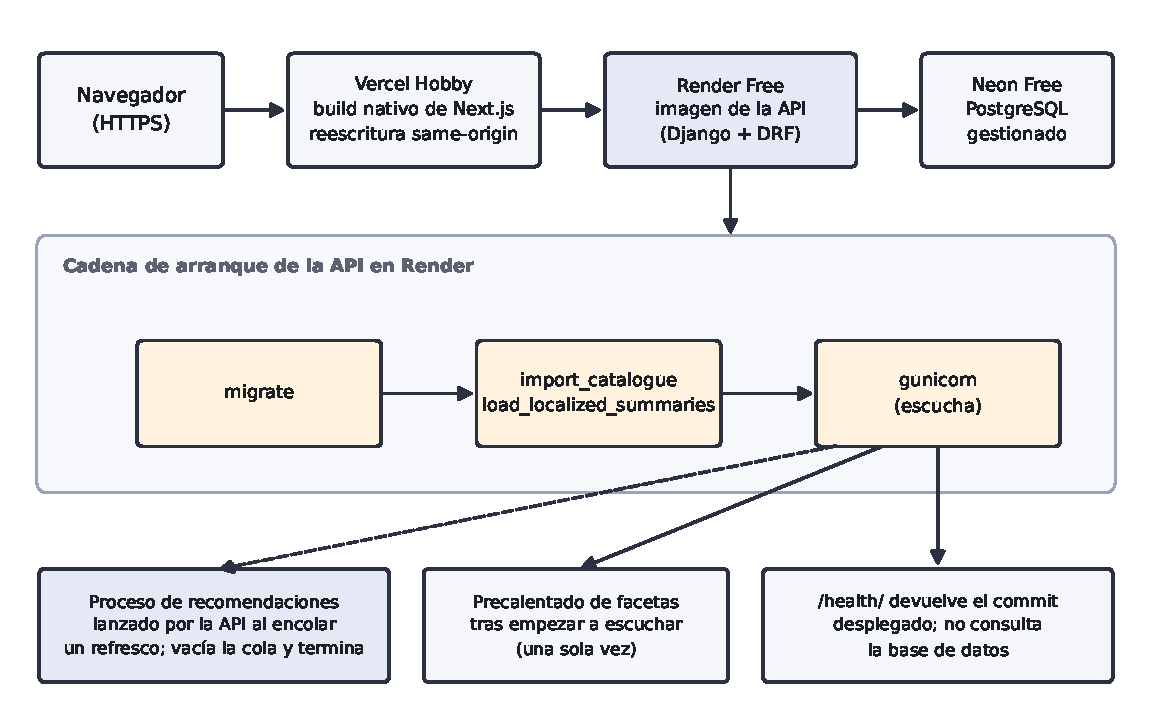
\includegraphics[width=0.92\textwidth]{figures/despliegue-flujo.pdf}
    \caption[Topología de despliegue público y cadena de arranque]{Topología de despliegue público, cadena de arranque en Render y procesos que cuelgan del servidor en marcha. Cada paso del arranque es idempotente y un paso fallido lo detiene. Docker Compose local (base de datos, API y frontend) construye las mismas imágenes sin depender de estos tres servicios.}
    \label{fig:despliegue-flujo}
\end{figure}

Docker Compose sigue siendo el entorno reproducible canónico
(Sección~\ref{sec:impl-entorno}). La equivalencia con el
despliegue público es funcional, de versiones y de commit, no de imagen byte a
byte ni de datos. El frontend público lo construye Vercel de forma nativa y no ejecuta la imagen de Docker
del frontend, una diferencia de despliegue documentada, no una divergencia de comportamiento; el corpus público
es un subconjunto del local, como recoge la Tabla~\ref{tab:local-publico}.
Si cualquier servicio gratuito duerme, cambia sus términos o desaparece, el entorno local sigue
disponible sin conexión. Los límites conocidos del nivel gratuito se declaran de forma
explícita: el servicio de la API en Render duerme tras quince minutos sin tráfico, de modo que
un visitante puede encontrar un arranque en frío de cerca de un minuto; las cuotas mensuales de
los tres proveedores pueden suspender un servicio y el nivel gratuito no promete copias de
seguridad ni restauración.

La demostración pública está en vivo desde el 5 de septiembre de 2026. En su primera versión servía la interfaz
anterior al rediseño contra el corpus curado de ciento cincuenta juegos de Wikidata. Desde el 5 de octubre de 2026 sirve
la interfaz rediseñada y un subconjunto del catálogo a escala real cargado en Neon, con las recomendaciones calculadas
por un proceso bajo demanda. No es el mismo catálogo que el del entorno local y la
Tabla~\ref{tab:local-publico} recoge la diferencia.

\begin{table}[H]
\centering
\begin{tabularx}{\textwidth}{ | L{0.26\textwidth} | Y | Y | }
    \hline
    \textbf{Aspecto} & \textbf{Entorno local (Docker)} & \textbf{Despliegue público} \\
    \hline
    Corpus gobernado visible en el catálogo & 190.479 obras & 32.550 juegos (el 17\,\%), más 10.714 DLC relacionados \\
    \hline
    Criterio del corpus & Corpus completo gobernado de la versión 2026.09.2 & Juegos con valoración de IGDB o con PopScore mayor que cero \\
    \hline
    Vectores de características & Uno por obra gobernada, varias versiones & Uno por juego publicado, solo la versión vigente \texttt{fs-v13} \\
    \hline
    Procesos de recomendación & Tres en paralelo, uno por cada variante publicada & Uno, lanzado bajo demanda, que procesa los trabajos de las tres variantes \\
    \hline
    Evaluación offline & Sí; de aquí salen los artefactos de esta memoria & No; se ejecuta solo en local \\
    \hline
    Tamaño de la base de datos & 3,77\,GB & 359\,MB (límite de Neon gratuito: 1\,GiB) \\
    \hline
    Disponibilidad & Mientras se ejecute Docker & La API duerme tras unos quince minutos sin tráfico \\
    \hline
\end{tabularx}
\caption{Diferencias entre el entorno local y el despliegue público, a 5 de octubre de 2026.}
\label{tab:local-publico}
\end{table}

El subconjunto público se eligió con un criterio explícito y reproducible: juegos con valoración de IGDB o con PopScore
mayor que cero, junto con los DLC relacionados con ellos. Ocupa 359\,MB de la gigabyte que ofrece Neon en el nivel
gratuito y los guiones que lo exportan y lo cargan están en \texttt{scripts/public-corpus/}. El corpus gobernado completo,
con los índices de las tablas que usa la API, no cabe en ese límite.

El nivel gratuito de Neon contabiliza horas de cómputo mientras la base está despierta, por lo que un proceso que
consultara la cola de recomendaciones cada pocos segundos la mantendría encendida las veinticuatro horas del día y
agotaría la cuota del mes. Por eso el despliegue no tiene ningún proceso permanente: cuando la API encola un refresco,
lanza un proceso corto que vacía la cola y termina, protegido por un candado de fichero para que nunca haya dos a la vez
y la base solo se consulta cuando alguien actúa. Se comprobó en producción con una cuenta desechable: la primera
recomendación de una cuenta nueva estuvo lista entre cuatro y seis minutos después y tras nueve minutos sin ninguna
petición Neon registró su suspensión.

Esta diferencia es una limitación del trabajo, no un detalle de despliegue. Los resultados de la evaluación offline del
Capítulo~\ref{cap:resultados} se calcularon sobre el corpus completo local, de modo que la web desplegada es una
demostración funcional del producto y no el entorno donde se midió. Las recomendaciones allí son además más lentas, porque
un único proceso comparte procesador y 512\,MB con la API. Los datos son de demostración: las cuentas no verifican el correo y
las claves son de demostración. Ampliar el despliegue al corpus gobernado completo exigiría una base de datos de mayor
capacidad, de pago y queda fuera del coste cero que fijó el diseño.

Este capítulo ha descrito la construcción, la verificación y el despliegue del sistema. El
capítulo siguiente presenta la evaluación experimental de los algoritmos de recomendación que
se ejecutan sobre él.

    \chapter{Evaluación y resultados}\label{cap:resultados}\label{cap:experimentos}

Con los dieciséis algoritmos ya formulados en la Sección~\ref{cap:algoritmos}, este capítulo los somete al protocolo de evaluación
sin conexión y presenta los resultados publicados junto con una discusión honesta de lo que permiten y de lo que no
permiten concluir. El énfasis no está en declarar un ganador, sino en dejar trazable cada cifra
hasta el corpus, la semilla, el reparto y la configuración exactos que la produjeron.

La evaluación se ejecuta sobre la misma plataforma descrita en los capítulos anteriores: los
usuarios sintéticos, sus bibliotecas y el corpus gobernado viven en la misma base de datos que
sirve la aplicación.

\section{Fundamentos de evaluación}\label{sec:exp-fundamentos}

La parte más delicada no es implementar los algoritmos, sino evaluarlos de forma
comparable~\cite{herlocker2004evaluating, gunawardana2015evaluating}. La literatura señala
varios riesgos recurrentes: ajustar los hiperparámetros sobre el conjunto de prueba, comparar
algoritmos con repartos o candidatas distintos, medir solo la precisión y olvidar la
cobertura, la diversidad o la novedad, o extraer conclusiones sobre personas reales a partir
de simulaciones sintéticas. El trabajo de Cremonesi y otros mostró además que las métricas de
error sobre la valoración predicha y las métricas de acierto sobre la lista recomendada
pueden ordenar los algoritmos de forma distinta~\cite{cremonesi2010performance}. La respuesta
metodológica aceptada es fijar por adelantado, de forma inmutable, el corpus, el reparto, las
exclusiones, las métricas, las semillas y el presupuesto de ajuste, antes de comparar nada.
El protocolo de SavePoint deja la comparación preparada y repetible, pero no debe confundirse
con una afirmación sobre usuarios reales: los resultados de este capítulo se miden sobre un
corpus y una población sintética concretos.

Evaluar un recomendador sin usuarios reales exige fijar por adelantado cinco decisiones: la
tarea concreta que se mide (recomendar los siguientes \(K\) ítems que a una persona le
interesarán, no predecir la nota exacta que pondría), el criterio de relevancia que separa un
acierto de un fallo, el conjunto de candidatas sobre el que compite cada algoritmo, la división
de los datos entre lo que el modelo puede ver y lo que se usa para medir y la forma de agregar
el resultado por usuario en una única cifra por algoritmo. SavePoint fija estas decisiones en
un protocolo versionado antes de ejecutar la comparación.

La precisión en \(K\) mide qué proporción de los \(K\) ítems recomendados resultan relevantes;
la exhaustividad en \(K\) mide qué proporción de todos los ítems relevantes aparecen entre
esos \(K\). Ninguna de las dos distingue la posición dentro de la lista: acertar en el primer
puesto cuenta igual que acertar en el último. Para corregir esa carencia se usa la ganancia
acumulada descontada normalizada~\cite{jarvelin2002cumulated}, que descuenta el valor
de un acierto cuanto más abajo aparece y lo normaliza frente al orden ideal posible. La
precisión media promedia, para cada usuario, la precisión acumulada en cada posición
donde hubo un acierto y después promedia ese valor entre usuarios; es sensible tanto a la
cantidad de aciertos como a su posición.

Estas cuatro métricas comparten una limitación de fondo: ninguna equivale a satisfacción
humana, porque miden coincidencia con un historial pasado, no si a la persona le va a gustar lo
recomendado. Por eso se completan con tres métricas de otra naturaleza. La diversidad mide
cuánto se parecen entre sí los ítems de una misma lista recomendada; la novedad mide cuánto se
aleja la recomendación de lo obvio o ya muy popular; y la cobertura mide qué proporción del
catálogo llega a aparecer alguna vez recomendada. Un recomendador que maximiza solo precisión
o nDCG puede hacerlo a costa de las tres, recomendando siempre lo mismo a todo el mundo; la
Sección~\ref{cap:algoritmos} explica cómo SavePoint reordena sus listas para compensarlo.

\section{Protocolo de evaluación}\label{sec:exp-protocolo}

La evaluación publicada se ejecutó offline con el corpus congelado \texttt{2026.09.2} (190.479 obras
gobernadas, Sección~\ref{sec:datos-congelacion}) y el conjunto de
características \texttt{fs-v12-curated-tags-idf} (Sección~\ref{cap:algoritmos} y
Tabla~\ref{tab:pesos-familia}); la revisión posterior \texttt{fs-v13} no se ha evaluado. La población experimental contiene 400 usuarios de prueba sintéticos, generados de forma determinista; 79 cumplen la elegibilidad del split de prueba. La población se reparte en dos cohortes: \texttt{active\_history\_10\_to\_20}, con los 390 usuarios que tienen una biblioteca de entre 10 y 20 entradas y \texttt{no\_history}, con los 10 de arranque en frío, que no tienen ítems relevantes y no se evalúan; los 79 usuarios evaluables pertenecen todos a la primera. Los perfiles se generan a partir de nueve arquetipos: dos sin historial (diez usuarios), tres de perfil inicial (cien), tres de usuario normal (doscientos cuarenta) y uno intensivo veterano (cincuenta). Los arquetipos con historial tienen bibliotecas de entre 10 y 20 entradas y varían el número de géneros preferidos, la generosidad al puntuar y la mezcla de estados; llevan el marcador \texttt{synthetic-eval-user} para no contaminar el baseline de popularidad de la aplicación. El protocolo v15 fija semilla, versiones, snapshots, hashes, candidatas y exclusiones antes de consumir el test. La semilla permite reproducir esta ejecución, pero no sustituye un estudio de sensibilidad con múltiples semillas.

El protocolo publicado, v15, usa \emph{leave-fraction-out} por usuario, no
\emph{leave-one-out}: retiene varios ítems relevantes por persona en lugar de uno solo. Una
obra relevante es una entrada terminada o valorada con al menos siete medios puntos, con un
piso adicional de calidad externa (valoración agregada de origen de al menos 70 puntos) sobre
las candidatas a retener. Para cada usuario, el runner localiza su etiqueta de contenido con
más peso en el perfil y retira de ella un \(\lceil 0{,}3\times\) tamaño del grupo de esa
etiqueta\(\rceil\) de obras, nunca menos de una, retrocediendo de una en una si la retirada
desplazara esa etiqueta del primer puesto del perfil restante. Cuando ese mecanismo no se
puede construir para un usuario (sin ninguna señal de etiqueta de contenido, o sin candidatas
que superen el piso de calidad), el runner recurre al \emph{leave-one-out} simple de un único
ítem en lugar de excluir a esa persona del estudio; solo queda fuera quien no tiene ningún
positivo elegible en absoluto. Sobre los setenta y nueve usuarios evaluables, este mecanismo
retuvo doscientos dos ítems en total, una media de 2{,}56 por usuario con un rango de uno a
cinco. Todos los algoritmos reciben el mismo manifiesto de candidatas; el diseño evita
filtración de datos: ningún ítem retenido participa en la construcción del perfil, mientras que su
presencia entre las candidatas permite medir si se recupera.

Se calcula \(K\in\{5,10,20\}\). Si \(R_u\) es el conjunto relevante retenido de un usuario y
\(L_u^K\) los primeros \(K\) ítems de su lista, \(Precision@K=|L_u^K\cap R_u|/K\) y
\(Recall@K=|L_u^K\cap R_u|/|R_u|\). Al retener varios ítems por usuario, \(Recall@K\) deja de
ser binario y se convierte en una fracción continua, lo que aporta más información por
comparación que el \emph{leave-one-out} de una sola versión anterior del protocolo. El nDCG
y el MAP se calculan sobre la misma
lista. El protocolo también conserva diversidad
intra-lista, novedad, coberturas y concentración cuando el artefacto permite estimarlas.

\subsection{Reparto de los usuarios y uso de la validación}\label{sec:exp-reparto}

Los 400 usuarios sintéticos se reparten por usuario, no por ítem, en tres subconjuntos disjuntos con una semilla
fija: 240 de entrenamiento, 80 de validación y 80 de prueba (Tabla~\ref{tab:exp-reparto}). Las métricas de este
capítulo se calculan solo sobre los usuarios de prueba; dentro de cada uno de ellos, el protocolo v15 retira después
la fracción de ítems relevantes descrita arriba.

\begin{table}[htp]
\centering
\small
\begin{tabularx}{\textwidth}{ | L{0.17\textwidth} | C{0.17\textwidth} | Y | }
    \hline
    \textbf{Partición} & \textbf{Usuarios} & \textbf{Papel en este capítulo} \\
    \hline
    Entrenamiento & 240 & Población de referencia del filtrado colaborativo por vecinos (\texttt{cf-user-knn-v1}) y base de frecuencias con la que se mide la novedad. No se evalúan. \\
    \hline
    Validación & 80 & Reservada para seleccionar configuraciones; no se ha utilizado para ello (véase más abajo). \\
    \hline
    Prueba & 80 (79 evaluados) & Comparación final de las dieciséis variantes, con un único consumo por versión del protocolo. \\
    \hline
\end{tabularx}
\caption{Reparto de los 400 usuarios sintéticos y papel de cada partición.}
\label{tab:exp-reparto}
\end{table}

\textbf{Por qué solo 79 de los 400 usuarios se evalúan.} Los 79 no son una selección de los 400 por falta de datos:
son la partición de prueba, de 80 usuarios, menos uno que no tiene ningún ítem relevante elegible. El artefacto lo
registra como 80 solicitados, 79 evaluados y 1 omitido. Los otros 320 usuarios, 240 de entrenamiento y 80 de
validación, no se evalúan en la comparación final por diseño, no por ser inservibles.

\textbf{Ajuste de hiperparámetros.} El protocolo declaró, antes de ejecutar nada, una rejilla de ajuste de como
máximo 31 configuraciones que debía puntuarse solo sobre validación con \(nDCG@10\), para bloquear la ganadora antes
de tocar la prueba. No se conserva ninguna ejecución de esa rejilla: todos los artefactos conservados corresponden a
la partición de prueba y no hay ninguno sobre validación. Los parámetros de las dieciséis variantes (los pesos por
familia, el \(\lambda\) de la reordenación, los pesos de PopScore y los demás) son decisiones de diseño justificadas
en la Sección~\ref{cap:algoritmos}, no valores seleccionados sobre validación. Por tanto no se ajustó ningún
hiperparámetro mediante una búsqueda sobre la prueba, pero tampoco se utilizó la validación para ello.

Esto no equivale a un aislamiento completo de la prueba. El protocolo se modificó de v12 a v15 después de ver los
resultados de prueba de las versiones anteriores (Sección~\ref{sec:exp-evolucion}), de modo que el consumo único de la
partición de prueba rige dentro de cada versión del protocolo, no entre versiones. Es una limitación del estudio y se
recoge entre las amenazas a la validez (Sección~\ref{sec:exp-amenazas}).

\section{Evolución del protocolo: tres intentos, no uno}\label{sec:exp-evolucion}\label{sec:exp-v15-fidelidad}

Los números de versión de esta sección designan el \emph{protocolo} de evaluación, no el conjunto de
características (v15 se calculó con \texttt{fs-v12}, Sección~\ref{cap:algoritmos}). El protocolo se versiona con un
número entero que sube cada vez que un cambio impide comparar sus resultados con los
de las versiones anteriores. La Tabla~\ref{tab:exp-versiones} resume las versiones, reconstruidas a partir del
historial del repositorio y de los documentos de verificación. Hasta v14 el esquema de partición fue siempre
\emph{leave-one-out}, con un único ítem retenido por usuario; lo que cambió fue la señal de calidad, la regla de
elegibilidad de las candidatas, el elenco de algoritmos, la población sintética y el piso de calidad. Con los 400
usuarios se ejecutaron sobre la partición de prueba v12, v13, v14 y v15, pero la ejecución de v13 se descartó por un
error del banco de pruebas, no del protocolo (candidatas duplicadas en las listas ordenadas): los resultados válidos
son los de v12, v14 y v15.

\begin{table}[htp]
\centering
\small
\begin{tabularx}{\textwidth}{ | C{0.13\textwidth} | C{0.13\textwidth} | Y | }
    \hline
    \textbf{Versión} & \textbf{Fecha (2026)} & \textbf{Qué cambió} \\
    \hline
    v1--v2 & 7--8 sep. & Congelación inicial del contrato: \emph{leave-one-out} por usuario, \(K \in \{5, 10, 20\}\) y \(nDCG@10\) como métrica titular. La versión v2 limita las candidatas a obras con valoración. Primera ejecución de prueba, con la población inicial (26 de 40 usuarios de prueba evaluables). \\
    \hline
    v3--v6 & 9 sep. & Similitud de contenido por facetas y señal de calidad con confianza, calibradas en varias iteraciones; v6 es la versión que congeló el documento del protocolo. \\
    \hline
    v7--v9 & 9 sep. & Peso de PopScore de 0,20, valoración bayesiana (contracción hacia la media del corpus con \(m = 25\)) y regla de elegibilidad: obra gobernada, con fecha no futura, valoración de usuarios y al menos cinco valoraciones totales. \\
    \hline
    v10 & 10 sep. & Señal final de valoración (calidad por confianza), reordenación híbrida con MMR y rejilla de ajuste de 31 configuraciones. \\
    \hline
    v11--v12 & 10 sep. & Unificación de las etiquetas curadas y congelación de las entradas del cálculo. v12 es el primer cálculo completo con los 400 usuarios. \\
    \hline
    v13 & 11 sep. & Población sintética regenerada, con todas las bibliotecas con historial de entre 10 y 20 entradas. Su ejecución de prueba se descartó: un error del banco de pruebas duplicaba candidatas en las listas de los algoritmos de contenido y desbordaba sus métricas; se conserva marcada como inválida y no es un resultado. \\
    \hline
    v14 & 11 sep. & Piso de calidad externa para el ítem retenido. Segundo cálculo completo. \\
    \hline
    v15 & 12 sep. & \emph{Leave-fraction-out} sobre la etiqueta dominante de cada usuario. Versión publicada. \\
    \hline
\end{tabularx}
\caption{Versiones del protocolo de evaluación.}
\label{tab:exp-versiones}
\end{table}

Los resultados de v15 no fueron el primer cálculo ejecutado hasta el final contra la partición de prueba: lo precedieron v12 y v14, cada uno consumido una sola vez, con sus resultados conservados sin alterar. La forma concreta de v15 (retención por fracción sobre una etiqueta propia de cada usuario, piso de calidad externa, población con mínimo garantizado) responde a dos problemas reales que esos intentos dejaron medidos, no a una elección de diseño arbitraria.

\textbf{El protocolo v12 (10 de septiembre de 2026)} fue el primer cálculo congelado hasta el final. Su
resultado no fue una comparación entre algoritmos, sino un hallazgo metodológico: el
setenta y cuatro por ciento de los setenta y tres usuarios evaluables de aquella partición
(cincuenta y cuatro de setenta y tres) caía en un modo de \enquote{historial insuficiente} del
recomendador de contenido en cuanto el \emph{leave-one-out} uno retiraba su único positivo
elegible, porque la población sintética de entonces no garantizaba un mínimo de positivos
por biblioteca. En ese modo, las diez variantes de contenido y sus derivadas dejaban de usar
similitud de etiquetas y colapsaban a la misma ordenación por valoración y popularidad que ya
usaban los métodos de referencia, de modo que quince de los dieciséis algoritmos publicaron precisión,
recall, nDCG y MAP exactamente en cero. La prueba de Friedman fue significativa
(\(\chi^2=30{,}00\), \(p=0{,}0119\), \(n=73\)), pero ninguna de las ciento veinte
comparaciones por pares sobrevivió la corrección de Holm: bajo ese protocolo, ningún
algoritmo era declarable superior a otro. Se verificó que no era un fallo del código de
puntuación (los vectores de contenido coincidían byte a byte con la caché versionada y el
conjunto de candidatas era idéntico para los dieciséis algoritmos), sino una interacción entre
dos piezas congeladas por separado: el generador de población sintética y el umbral de
arranque en frío del recomendador de contenido.

Corregir esa interacción exigió dos cambios sucesivos. El primero (protocolo v13), con la población
rediseñada, amplió el tamaño de biblioteca sintética, ensanchó la franja de popularidad de
origen y garantizó un mínimo de cinco positivos elegibles por biblioteca. La ejecución de prueba de v13 no es
válida: un error del banco de pruebas duplicaba candidatas en las listas de los algoritmos de contenido (una obra
con varias etiquetas curadas aparecía varias veces) y desbordaba sus métricas, por lo que se descartó y se conservó
solo como evidencia del fallo. Por eso el efecto de la población rediseñada se midió en la ejecución de v14, que ya
reúne ambos cambios: el modo de historial insuficiente dejó de afectar a la partición de prueba y pasó del setenta y
cuatro por ciento de los usuarios a un cero por ciento. El segundo cambio añadió, sobre esa
población ya corregida, un piso de calidad externa (valoración agregada de origen de al menos
setenta puntos) al ítem que la retención de uno podía retirar, para que el positivo
retenido no dependiera solo del gusto personal simulado sino también de una señal de calidad
independiente, cerrando un sesgo de popularidad conocido en la literatura de evaluación de
recomendadores~\cite{cremonesi2010performance}.

\textbf{El protocolo v14 (11 de septiembre de 2026)}, con esos dos cambios ya aplicados, sí produjo un
ganador defendible: \texttt{hybrid-weighted-cf-v1} (\(nDCG@10=0{,}1526\)) y
\texttt{content-cbf-weighted-v1} (\(0{,}1452\)) superaron con significación a los métodos de referencia y
a \texttt{recency-v1}, con catorce de las ciento veinte comparaciones por pares significativas
tras Holm, frente a cero en v12 (\(\chi^2=105{,}28\), \(p=1{,}29\times10^{-15}\), \(n=79\)). La
diversidad intra-lista y la concentración de recomendaciones mejoraron en la misma medida: el
índice de concentración de Herfindahl-Hirschman (HHI) pasó de un rango de 0,55 a 0,71 en v12, propio
de un catálogo minúsculo de recomendaciones repetidas, a un rango de 0,005 a 0,03, consecuencia
directa de que el contenido ya no colapsaba a la misma alternativa de respaldo que los métodos de referencia. Aun
así, v14 seguía reteniendo un único ítem por usuario mediante retención de uno: cada
comparación por usuario solo podía acertar o fallar una vez, lo que limitaba cuántas
diferencias entre algoritmos podían alcanzar significación. El colaborativo puro, por ejemplo,
no llegó a diferenciarse de forma significativa de ningún otro algoritmo en v14, pese a tener
un nDCG@10 más bajo que las variantes de contenido con mejor combinación.

Ese límite de potencia estadística, no un defecto de v14, es lo que motivó el cambio final a
retención por fracción por etiqueta dominante propia de cada usuario que define el
protocolo v15: retener varios positivos por persona en lugar de uno solo da a cada comparación
más información por usuario sin necesidad de una población mayor. El resultado, ya presentado
en la Sección~\ref{sec:exp-significacion}, fue el esperado: de catorce comparaciones
significativas en v14 a cincuenta y cuatro en v15, con una diferenciación entre contenido y
colaborativo puro que v12 y v14 no tenían potencia estadística suficiente para establecer.
Los tres protocolos válidos y sus artefactos quedan versionados sin modificar (la ejecución descartada de v13 se
conserva aparte, marcada como inválida): v15 no invalida ni
reescribe los resultados de v12 o v14, los sustituye como publicación vigente por haber
corregido, de forma medida y documentada, los problemas que los dos intentos anteriores dejaron
al descubierto.

Conviene defender que v15 se acerca más a una prueba realista de lo que los algoritmos hacen, no que se ajusta para producir números más altos, porque corrige tres formas en las que v12 y v14 se apartaban de la literatura y del propio sistema. La primera es de encuadre: retirar y recuperar un subconjunto de valoraciones, en lugar de un único ítem, es la generalización natural del esquema \emph{All-but-N}, nombrado así desde Breese, Heckerman y Kadie~\cite{breese1998empirical} y sistematizado por Herlocker et al.~\cite{herlocker2004evaluating}, del que el \emph{leave-one-out} de los protocolos v6 a v14 (Tabla~\ref{tab:exp-versiones}) es el caso \(N=1\); v15 solo calcula \(N\) por usuario, en proporción al tamaño de su grupo de obras con la etiqueta dominante. La segunda es de fidelidad a la señal que el sistema usa: \texttt{facet\_similarity()}, el código de puntuación de los dieciséis algoritmos, combina cada familia de faceta como una suma ponderada, nunca como un único rasgo ganador, de modo que el 21{,}3\,\% de los casos verificados antes de congelar el protocolo en los que la etiqueta retirada deja de ser la primera del perfil recalculado no invalida la prueba: el perfil sigue apoyándose en ella con menos peso~\cite{pazzani2007content} y exigir lo contrario habría excluido usuarios que el sistema sí atiende. La tercera es de inclusión: el usuario para el que el mecanismo por fracción no se puede construir cae al \emph{leave-one-out} simple en lugar de quedar fuera, lo que evita quedarse solo con los usuarios más fáciles de evaluar y llamar a eso representativo.

Ninguno de los tres argumentos convierte v15 en evidencia sobre jugadores reales, como recuerda la Sección~\ref{sec:exp-amenazas}. Lo que establecen es que, dentro de la simulación, v15 mide la pregunta que se propone medir (¿recupera el sistema contenido afín al gusto que la propia biblioteca del usuario ya demuestra?) con más fidelidad al mecanismo de puntuación real y con menos artefactos de diseño heredados que v12 o v14, no solo con mejores cifras.

\section{Resultados publicados}\label{sec:exp-resultados}\label{sec:exp-exito}

La Tabla~\ref{tab:resultados-ndcg10} resume \(nDCG@10\), MAP@10 y el tiempo de pared de cada algoritmo, en segundos, tal como los registra el artefacto v15. Las métricas son las de los 79 usuarios evaluables, que pertenecen a la cohorte \texttt{active\_history\_10\_to\_20}; esa cohorte no es el conjunto de los 79, sino los 390 usuarios sintéticos con una biblioteca de entre 10 y 20 entradas; solo se evalúan los 79 que caen en la partición de prueba y tienen al menos un ítem relevante elegible. El tiempo es la duración del proceso que ejecutó cada algoritmo, no un tiempo por usuario. Se muestra una tabla compacta para evitar repetir cuatro métricas por tres valores de \(K\); el artefacto versionado \texttt{evaluation-400-test-2026-09-12-v15.artifact.json} y su transcripción en \texttt{docs/verification/evaluation-cohorts-400-test-2026-09-12-v15.md} preservan la transcripción completa para \(K=5,10,20\).

\begin{table}[H]
\centering
\caption[Resultados v15 publicados para los 79 usuarios evaluables]{Resultados v15 publicados (conjunto de características \texttt{fs-v12}) para los 79 usuarios evaluables de la cohorte \texttt{active\_history\_10\_to\_20}, con el tiempo de pared de cada algoritmo en segundos. No son resultados con usuarios reales.}\label{tab:resultados-ndcg10}
\small
\renewcommand{\arraystretch}{1.2}
\setlength{\tabcolsep}{3pt}
\begin{tabularx}{\textwidth}{@{}>{\ttfamily\footnotesize\raggedright\arraybackslash}p{0.385\textwidth}Y>{\raggedleft\arraybackslash}p{0.105\textwidth}>{\raggedleft\arraybackslash}p{0.105\textwidth}>{\raggedleft\arraybackslash}p{0.105\textwidth}@{}}
\textnormal{Algoritmo} & \textnormal{Familia} & \textnormal{\footnotesize nDCG@10} & \textnormal{\footnotesize MAP@10} & \textnormal{\footnotesize Tiempo (s)} \\
\hline
random-v1 & referencia & 0,00000 & 0,00000 & 25,1 \\
popularity-v1 & referencia & 0,00340 & 0,00098 & 5,1 \\
content-cbf-weighted-v1 & contenido & 0,17245 & 0,10878 & 492,8 \\
content-cbf-multiplicative-v1 & contenido & 0,08558 & 0,05934 & 491,4 \\
content-cbf-twostage-v1 & contenido & 0,11724 & 0,06767 & 488,5 \\
content-cbf-neg-v1 & contenido & 0,11778 & 0,07368 & 488,2 \\
content-cbf-weighted-pop-v1 & contenido + popularidad & 0,15181 & 0,09826 & 484,0 \\
content-cbf-multiplicative-pop-v1 & contenido + popularidad & 0,08517 & 0,05898 & 480,4 \\
content-cbf-twostage-pop-v1 & contenido + popularidad & 0,11410 & 0,06551 & 484,2 \\
content-cbf-neg-pop-v1 & contenido + popularidad & 0,09936 & 0,06134 & 483,9 \\
recency-v1 & contenido + novedad & 0,00594 & 0,00422 & 427,6 \\
content-cbf-mmr-v1 & contenido + diversidad & 0,13888 & 0,08685 & 483,3 \\
content-cbf-mmr-pop-v1 & contenido + diversidad & 0,13824 & 0,09353 & 481,7 \\
cf-user-knn-v1 & colaborativo & 0,02098 & 0,01099 & 16,8 \\
hybrid-weighted-cf-v1 & híbrido & 0,16989 & 0,10758 & 439,7 \\
hybrid-mmr-v1 & híbrido + diversidad & 0,15913 & 0,09741 & 493,1 \\
\end{tabularx}
\end{table}

La Tabla~\ref{tab:ndcg-todos-k} conserva \(nDCG\) en los tres cortes solicitados para el catálogo completo de variantes v15. Precision, recall y MAP permanecen en el artefacto y en la matriz de algoritmos para evitar una tabla de dieciséis filas y doce métricas que perdería legibilidad.

\begin{table}[H]
\centering
\caption{nDCG publicado por algoritmo y corte $K$ en v15 (\texttt{fs-v12}).}\label{tab:ndcg-todos-k}
\tablecompact
\begin{tabularx}{\textwidth}{@{}>{\ttfamily\raggedright\arraybackslash}p{0.45\textwidth}Yrrr@{}}
\textnormal{Algoritmo} & \textnormal{Familia} & \textnormal{$K=5$} & \textnormal{$K=10$} & \textnormal{$K=20$} \\
\hline
random-v1 & referencia & 0,00000 & 0,00000 & 0,00000 \\
popularity-v1 & referencia & 0,00191 & 0,00340 & 0,00340 \\
content-cbf-weighted-v1 & contenido & 0,14114 & 0,17245 & 0,18987 \\
content-cbf-multiplicative-v1 & contenido & 0,07707 & 0,08558 & 0,10241 \\
content-cbf-twostage-v1 & contenido & 0,08827 & 0,11724 & 0,14002 \\
content-cbf-neg-v1 & contenido & 0,09656 & 0,11778 & 0,12992 \\
content-cbf-weighted-pop-v1 & contenido + popularidad & 0,13179 & 0,15181 & 0,17409 \\
content-cbf-multiplicative-pop-v1 & contenido + popularidad & 0,07677 & 0,08517 & 0,10200 \\
content-cbf-twostage-pop-v1 & contenido + popularidad & 0,08338 & 0,11410 & 0,14538 \\
content-cbf-neg-pop-v1 & contenido + popularidad & 0,08602 & 0,09936 & 0,11582 \\
recency-v1 & contenido + novedad & 0,00594 & 0,00594 & 0,00594 \\
content-cbf-mmr-v1 & contenido + diversidad & 0,11600 & 0,13888 & 0,16160 \\
content-cbf-mmr-pop-v1 & contenido + diversidad & 0,12211 & 0,13824 & 0,15362 \\
cf-user-knn-v1 & colaborativo & 0,01585 & 0,02098 & 0,03163 \\
hybrid-weighted-cf-v1 & híbrido & 0,14305 & 0,16989 & 0,18962 \\
hybrid-mmr-v1 & híbrido + diversidad & 0,13195 & 0,15913 & 0,17401 \\
\end{tabularx}
\end{table}

La diferencia numérica más visible en \(nDCG@10\) aparece entre \texttt{content-cbf-weighted-v1} y los métodos de referencia. El híbrido ponderado queda próximo a esa variante de contenido, mientras que el colaborativo aislado recupera menos positivos bajo esta partición. Esta observación es interna al artefacto: no prueba que contenido sea superior en una comunidad real, ni que los pesos del híbrido sean óptimos. De las tres variantes que publica la aplicación
(Sección~\ref{sec:alg-publicadas}), \texttt{content-cbf-weighted-v1} obtiene el mejor
\(nDCG@10\) (0{,}17245), \texttt{content-cbf-mmr-pop-v1} queda algo por debajo (0{,}13824) y
\texttt{recency-v1} apenas llega a 0{,}00594, lo que es coherente con su papel de variante de
descubrimiento, que prioriza la novedad sobre la afinidad. Para \(K=5\), \texttt{hybrid-weighted-cf-v1} publica \(nDCG=0{,}14305\), frente a \(0{,}14114\) de la variante ponderada. Para \(K=20\), la variante ponderada publica \(0{,}18987\) y el híbrido ponderado \(0{,}18962\). La proximidad de esas cifras ilustra por qué no basta con mirar la diferencia numérica sin contrastarla; la Sección~\ref{sec:exp-significacion} retoma esta misma comparación con una prueba estadística. El método de referencia aleatorio permanece en cero en la cohorte publicada; popularidad alcanza \(0{,}00340\) en \(nDCG@10\), lo que contextualiza la señal de contenido pero no mide utilidad subjetiva. La Figura~\ref{fig:ndcg-algoritmos} ordena los dieciséis algoritmos por \(nDCG@10\) y señala las tres variantes que publica la aplicación.

\begin{figure}[htp]
    \centering
    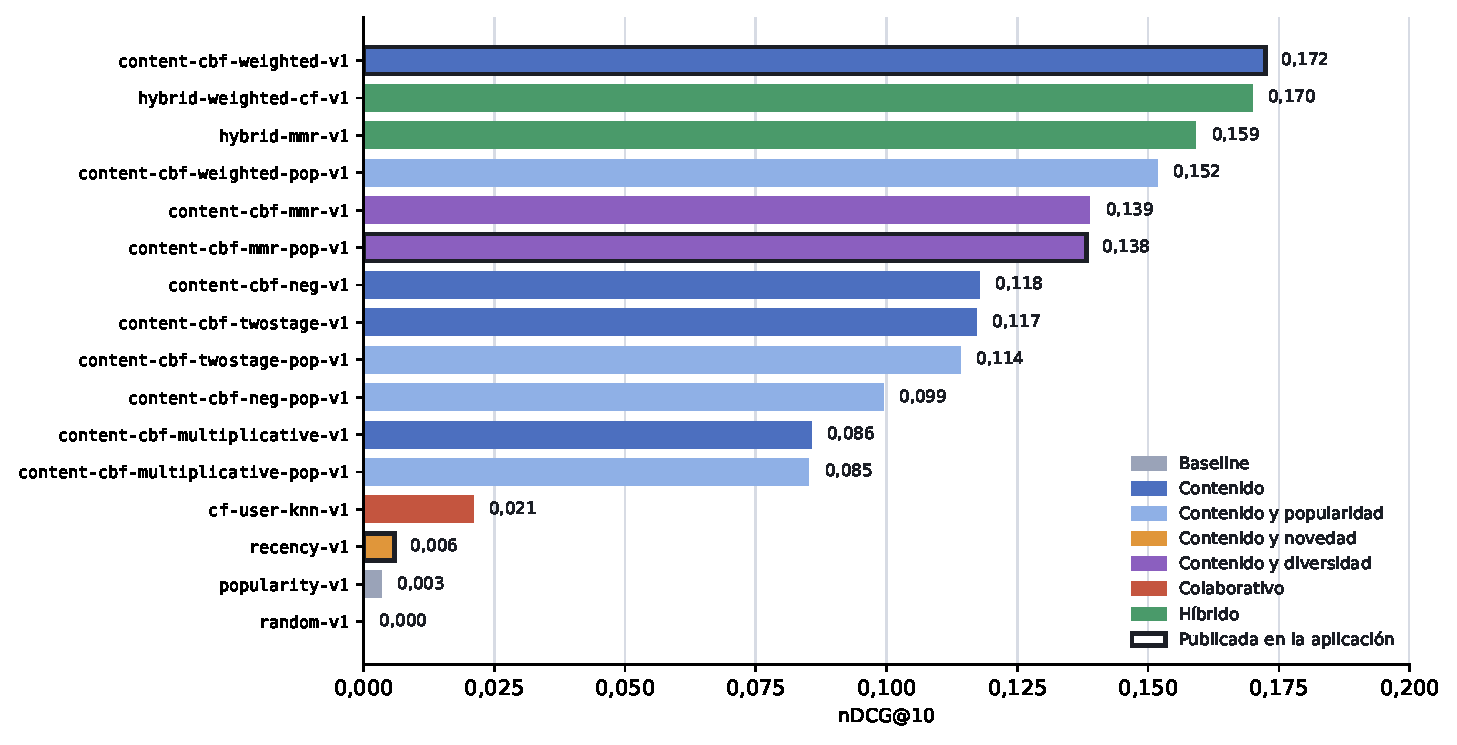
\includegraphics[width=0.9\textwidth]{figures/ndcg-algoritmos.pdf}
    \caption{\(nDCG@10\) de los dieciséis algoritmos en la evaluación v15 (\texttt{fs-v12}), por familia. El borde grueso marca las tres variantes publicadas en la aplicación.}
    \label{fig:ndcg-algoritmos}
\end{figure}

nDCG y MAP resumen la recuperación en una única cifra por algoritmo, pero no responden
directamente a la pregunta más intuitiva: ¿a cuántas personas le funcionó? La
Tabla~\ref{tab:exito-usuarios} lo hace explícito para \(K=10\), sobre los doscientos dos
ítems retenidos y los setenta y nueve usuarios evaluables.

\begin{table}[H]
\centering
\caption{Éxitos por algoritmo a \(K=10\): ítems retenidos recuperados sobre 202; usuarios
que recuperaron al menos uno de los suyos sobre 79.}\label{tab:exito-usuarios}
\small
\begin{tabularx}{\textwidth}{@{}>{\ttfamily\raggedright\arraybackslash}X C{0.22\textwidth} C{0.25\textwidth}@{}}
\textnormal{Algoritmo} & \textnormal{Ítems@10 (/202)} & \textnormal{Usuarios\(\geq\)1@10 (/79)} \\
\hline
content-cbf-weighted-v1 & 48 & 39 (49\,\%) \\
hybrid-weighted-cf-v1 & 48 & 38 (48\,\%) \\
hybrid-mmr-v1 & 42 & 35 (44\,\%) \\
content-cbf-weighted-pop-v1 & 38 & 34 (43\,\%) \\
content-cbf-mmr-v1 & 36 & 32 (41\,\%) \\
content-cbf-neg-v1 & 34 & 28 (35\,\%) \\
cf-user-knn-v1 & 7 & 7 (9\,\%) \\
popularity-v1 & 2 & 2 (3\,\%) \\
recency-v1 & 1 & 1 (1\,\%) \\
random-v1 & 0 & 0 (0\,\%) \\
\end{tabularx}
\end{table}

Leída así, la mejor variante de contenido devuelve al menos uno de los juegos retenidos del
usuario, dentro de las diez primeras posiciones, casi a la mitad de las personas evaluables
(49\,\%), frente al 9\,\% del colaborativo puro y el 3\,\% o menos de los métodos de referencia; a
\(K=20\) esa cifra sube al 58\,\% para \texttt{content-cbf-weighted-v1} (cuarenta y seis de
setenta y nueve usuarios). Esta tasa de éxito por usuario y el \(nDCG@10\) de la
Tabla~\ref{tab:resultados-ndcg10} miden cosas distintas y no deben confundirse: la primera
cuenta aciertos binarios por persona, mientras que la segunda además descuenta la posición
exacta del acierto dentro de la lista, por lo que una tasa de éxito alta no implica un nDCG
igual de alto si los aciertos tienden a aparecer hacia el final del top-\(K\) en vez de al
principio.

\section{Significación estadística}\label{sec:exp-significacion}

Las diferencias de la Tabla~\ref{tab:resultados-ndcg10} se sometieron a contraste antes de
interpretarlas, con una cadena de pruebas pensada para el caso en que dieciséis algoritmos se
miden sobre exactamente los mismos setenta y nueve usuarios (medidas repetidas, no muestras
independientes) y se quiere comparar cada par sin inflar el número de falsos positivos que
salen solo por probar muchas comparaciones a la vez. La cadena tiene cuatro piezas, todas ellas
procedimientos estadísticos estándar aplicados a este problema concreto, no invenciones del
proyecto.

Primero, una prueba de \textbf{Friedman} sirve de ómnibus: comprueba, con un único contraste,
si existe alguna diferencia entre los dieciséis algoritmos antes de gastar el presupuesto de
comparaciones en mirar pares sueltos. Es no paramétrica (no asume que los valores de nDCG se
distribuyan de forma normal, algo que no se puede dar por hecho con solo setenta y nueve
observaciones) y adecuada para medidas repetidas: cada usuario aporta una clasificación entre los
dieciséis algoritmos; la prueba contrasta si esas clasificaciones son consistentes entre sí. Sobre
\(nDCG@10\), rechaza la hipótesis de igualdad con \(\chi^2=258{,}07\) y
\(p=2{,}69\times10^{-46}\).

Segundo, confirmada la existencia de alguna diferencia, cada uno de los ciento veinte pares
posibles de algoritmos se contrasta con una prueba de \textbf{Wilcoxon de rangos con signo
pareada}: para cada usuario se calcula la diferencia de \(nDCG@10\) entre los dos algoritmos
del par; la prueba comprueba si esas diferencias pareadas se alejan de cero de forma
consistente, sin asumir tampoco su distribución. Es la elección natural aquí porque los dos
algoritmos de cada par se miden sobre las mismas setenta y nueve personas, no sobre grupos
distintos.

Tercero, probar ciento veinte pares a la vez con un umbral \(p<0{,}05\) fijo produciría, solo
por azar, varios falsos positivos aunque ningún algoritmo fuera realmente distinto de otro
(el problema de comparaciones múltiples). La \textbf{corrección de Holm} ajusta el umbral de
significación de cada una de las ciento veinte comparaciones, ordenadas de menor a mayor \(p\)
sin corregir, de forma escalonada y más potente que una corrección de Bonferroni simple sin
dejar de controlar el error de tipo I acumulado. Cincuenta y cuatro de las ciento veinte
comparaciones siguen siendo significativas después de este ajuste.

Cuarto, además del contraste de hipótesis, el artefacto conserva un \textbf{intervalo de
confianza por remuestreo BCa} (corregido por sesgo y acelerado, dos mil
remuestreos, confianza del 95\,\%, semilla fija) para el \(nDCG@10\) de cada algoritmo, que da
un rango de valores plausibles en lugar de una única cifra puntual y no exige asumir ninguna
forma concreta para la distribución del estadístico. La Tabla~\ref{tab:significacion} recoge
las comparaciones por pares más relevantes para la narrativa de este capítulo; la lista
completa de las ciento veinte vive en el artefacto versionado.

\begin{table}[H]
\centering
\caption{Comparaciones por pares más relevantes sobre \(nDCG@10\), con corrección de Holm
sobre las ciento veinte comparaciones totales.}\label{tab:significacion}
\small
\begin{tabularx}{\textwidth}{@{}Yrr@{}}
\textnormal{Comparación} & \textnormal{\(\Delta\) nDCG@10} & \textnormal{\(p\) ajustado} \\
\hline
content-cbf-weighted-v1 frente a random-v1 & +0{,}1725 & 0{,}00001 \\
content-cbf-weighted-v1 frente a popularity-v1 & +0{,}1691 & 0{,}00001 \\
hybrid-weighted-cf-v1 frente a random-v1 & +0{,}1699 & 0{,}00001 \\
cf-user-knn-v1 frente a content-cbf-weighted-v1 & \(-\)0{,}1515 & 0{,}00004 \\
cf-user-knn-v1 frente a hybrid-weighted-cf-v1 & \(-\)0{,}1489 & 0{,}00004 \\
\end{tabularx}
\end{table}

Dos lecturas se derivan de este contraste. La primera es que tanto las variantes de contenido
como los híbridos superan a los dos métodos de referencia y a \texttt{recency-v1} con significación
sobrada, lo que sí permite descartar el azar como explicación de esas diferencias concretas,
bajo este corpus y esta población. La segunda, nueva en este protocolo frente a versiones
anteriores, es que el colaborativo puro (\texttt{cf-user-knn-v1}) resulta significativamente
peor que ocho de las diez variantes de contenido, una diferenciación que la potencia
estadística de protocolos previos no alcanzaba a establecer con esta claridad. Esa lectura
tiene un matiz importante: esta prueba mide específicamente la recuperación de obras de la
etiqueta de contenido dominante del perfil de cada usuario y \texttt{cf-user-knn-v1} no usa
etiquetas en absoluto, sino similitud de patrones de valoración entre usuarios. La diferencia
es real y significativa, pero mide precisamente el terreno que la señal colaborativa no
modela; no es evidencia de que el filtrado colaborativo sea inferior en una tarea distinta,
como recuperar valoraciones de usuarios con gustos parecidos sin restricción de género. Los
híbridos combinan ambas señales en parte por esta razón: para no depender de ninguna de las
dos en solitario.

\section{Diversidad, cobertura y amenazas a la validez}\label{sec:exp-amenazas}

MMR introduce un objetivo distinto de la recuperación puntual: reducir redundancia entre elementos ya seleccionados. Sus resultados deben leerse junto con diversidad intra-lista, novedad, cobertura del catálogo, cobertura de predicción y HHI cuando el artefacto los publica. Una mejora de diversidad no compensa automáticamente una pérdida de nDCG, ni la métrica de acierto debe ocultar concentración. SavePoint mantiene estas medidas separadas para que el compromiso sea auditable. Con \(K=10\), la diversidad intra-lista de \texttt{content-cbf-weighted-v1} es 0,531 y sube a 0,652 en \texttt{content-cbf-mmr-v1}, mientras que su \(nDCG@10\) baja de 0,1725 a 0,1389; en el híbrido, de 0,532 a 0,655 de diversidad y de 0,1699 a 0,1591 de \(nDCG@10\). La cobertura es baja en todos los algoritmos: la mejor variante de contenido recomienda 241 de las 13.618 obras candidatas (el 1,77\,\%) entre los 79 usuarios y la popularidad solo 11 (el 0,08\,\%), con un HHI de 0,0988 frente a 0,0132 de la variante de contenido y de 0,0765 del colaborativo, que también concentra. La cobertura de predicción es completa (1,00) en los dieciséis algoritmos.

Las amenazas principales son población sintética, un solo consumo de la prueba y dependencia de
metadatos externos gobernados. El corpus y la versión inmutable son fortalezas de reproducibilidad,
pero acotan la generalización: la significación estadística de la Sección~\ref{sec:exp-significacion}
respalda que las diferencias observadas no son ruido bajo este corpus y esta población, no
que se sostengan sobre usuarios reales. Un estudio posterior debería incluir más semillas,
sensibilidades de hiperparámetros, datos observados con consentimiento y evaluación con
participantes, sin mutar el artefacto v15 ya publicado.

Este capítulo ha presentado la evaluación experimental de los algoritmos. El capítulo siguiente
cierra la memoria con el grado de cumplimiento de los objetivos y las líneas de continuación.

    \chapter{Conclusiones y continuidad}\label{cap:conclusiones}

Este capítulo cierra la memoria. Valora el grado de cumplimiento de los objetivos fijados en
el Capítulo~\ref{cap:introduccion}, resume las aportaciones del trabajo, declara sus
limitaciones sin suavizarlas y esboza las líneas de continuidad que el sistema deja abiertas.

\section{Grado de cumplimiento de los objetivos}\label{sec:conc-objetivos}

El objetivo general, construir una plataforma de catalogación que funcionara también como
banco de pruebas reproducible de recomendación, se cumple en lo esencial, con las salvedades que se detallan a
continuación. El catálogo tiene identidad canónica propia, procedencia por obra y licencia documentada, a escala
real sobre el catálogo importado de IGDB en el entorno local; el despliegue público solo sirve un subconjunto de
él. Una persona usuaria puede mantener su lista de pendientes, valorar juegos e inventariar copias físicas y
digitales con su formato y su edición, con privacidad de perfil y relaciones sociales cuya autorización se resuelve
en el backend. El protocolo de evaluación offline quedó congelado, versionado y probado antes de ejecutar ninguna
comparación, aunque se revisó entre versiones después de ver resultados de la partición de prueba
(Sección~\ref{sec:exp-evolucion}). Esa comparación se llevó a cabo: las tres familias de recomendación
(basada en contenido, colaborativa e híbrida), descritas con su formulación completa en la
Sección~\ref{cap:algoritmos}, se compararon bajo ese protocolo en el
Capítulo~\ref{cap:resultados} frente a los baselines de referencia, pero con usuarios sintéticos y una única
semilla, de modo que sus conclusiones valen para esa población y no para personas reales.

Por eso el cumplimiento no es íntegro. Quedan pendientes, de forma parcial, dos piezas del contrato de evaluación:
repetir la comparación con varias semillas y retroproyectar sobre la ejecución v15 la captura de entorno y consumo de
recursos. A ellas se suman tres carencias que la Sección~\ref{sec:conc-limitaciones} declara: la rejilla de ajuste
de hiperparámetros prevista sobre la partición de validación no se ejecutó, el conjunto de características vigente
(\texttt{fs-v13}) no se ha evaluado y el despliegue público no reproduce el corpus completo. Cada incremento del
sistema se cerró con sus criterios de éxito verificados de forma independiente, según la disciplina descrita en el
Capítulo~\ref{cap:gestion}; eso acredita que se cumplieron los criterios fijados, no que el sistema esté libre de
las limitaciones anteriores.

\section{Limitaciones y trabajo futuro}\label{sec:conc-limitaciones}\label{sec:conc-trabajo-futuro}

Las limitaciones conocidas se declaran sin ocultarlas. La evidencia experimental publicada
procede de una única ejecución del test sobre usuarios sintéticos, setenta y nueve de ellos
evaluables, con una sola semilla: es suficiente para comparar algoritmos entre sí bajo un
protocolo común, con significación estadística ya calculada sobre esa muestra (bootstrap BCa,
Friedman, Wilcoxon y corrección de Holm), pero no permite afirmar que esa significación sea
estable frente a otra semilla o a otra población sintética sin repetir el experimento. La
cobertura de valoraciones externas del catálogo es parcial, como corresponde a una fuente
agregada de terceros y no a un panel de crítica propio; esa parcialidad se propaga, de forma
documentada, a cualquier señal de calidad externa que la use. La captura de entorno de
ejecución y consumo de recursos, ya disponible en el ejecutor paralelo para comparaciones
futuras, no se retroproyectó sobre la ejecución v15 ya cerrada, de modo que esa ejecución
concreta carece de ese detalle. Tampoco se ha evaluado todavía el conjunto de características
\texttt{fs-v13}, posterior a esa ejecución: las cifras publicadas corresponden a \texttt{fs-v12}
(Sección~\ref{cap:algoritmos}). La rejilla de ajuste de hiperparámetros que el protocolo declaró para la partición de
validación no se ejecutó y el protocolo cambió de versión después de ver resultados de prueba, de modo que el consumo
único de esa partición rige dentro de cada versión y no entre ellas (Sección~\ref{sec:exp-reparto}). El despliegue público, descrito en la
Sección~\ref{cap:despliegue}, sirve un subconjunto del catálogo a escala real (32.550 de las 190.479 obras
gobernadas, el 17\,\%) y no el corpus completo, que no cabe en el nivel gratuito de la base de datos; la evaluación
offline se midió en el entorno local, no en el desplegado.

El banco de pruebas que esta memoria deja construido y ya explotado habilita líneas de
continuación concretas, no genéricas. La primera es repetir el protocolo publicado con nuevas
semillas y con cohortes sintéticas adicionales, para separar lo que es una diferencia
consistente entre algoritmos de lo que podría ser ruido de una única muestra y aplicar sobre la nueva ejecución la captura de entorno y consumo de recursos que el
ejecutor paralelo ya sabe registrar. La segunda es estudiar la sensibilidad del sistema a sus propios
hiperparámetros locales (los pesos de familia de facetas, la mezcla híbrida, el factor de
diversidad), en lugar de tratarlos como constantes fijadas de una vez.

Fuera del núcleo de recomendación, el producto deja cinco líneas abiertas. La primera es contrastar los algoritmos
con personas reales: la comparación publicada usa solo usuarios sintéticos y una prueba con un grupo pequeño que
usara la aplicación y valorara las recomendaciones daría una primera señal de hasta qué punto las conclusiones se
trasladan, algo que esta memoria no puede ofrecer. La segunda es completar la gestión de cuentas con verificación
de correo, recuperación de contraseña y una política de contraseñas común al registro y al cambio; hoy no existen
y por eso las cuentas del despliegue público son de demostración. La tercera es escalar el despliegue: ampliarlo al
corpus gobernado completo con una base de datos de mayor capacidad, dedicar un proceso de recomendación a cada
algoritmo, como ya hace el entorno local y servir las lecturas públicas del catálogo desde la caché en el borde de
Vercel. La cuarta es importar la colección desde una cuenta de Steam, para que quien ya tiene una biblioteca grande
no tenga que registrarla juego a juego; exigiría reconciliar los títulos de Steam con las obras canónicas del
catálogo, un problema de identidad semejante al que ya hubo que resolver entre Wikidata e IGDB y respetar los
términos de uso de la API de Steam y la privacidad del perfil. La quinta es una importación diaria del catálogo que
lo mantenga actualizado; como la evaluación depende de un corpus congelado, cada importación debería producir una
nueva versión del corpus, sin alterar las que ya usan los artefactos publicados.

Cualquier extensión de este trabajo deberá crear su propio protocolo y su propio artefacto
versionado, sin alterar de forma retroactiva la evidencia ya publicada.

\section{Aportaciones y valoración final}\label{sec:conc-aportaciones}\label{sec:conc-cierre}

Las tres aportaciones anunciadas en la Sección~\ref{sec:contexto-problema} quedan entregadas.
El producto está construido, verificado y documentado. El banco de pruebas está explotado: un
corpus citable, una población sintética documentada y un protocolo offline congelado sostienen
una comparación real entre dieciséis algoritmos, con sus artefactos, semillas y
configuraciones conservados para que un tercero pueda reproducir cada cifra publicada. Y la
metodología de ingeniería que gobernó el proyecto, versionada en el repositorio con su árbol
de planificación, sus registros de decisión y su registro de agentes, permite reconstruir el
rastro completo de decisiones. Así, el trabajo entrega las dos mitades de la idea de la que
parte SavePoint: un producto de catalogación y un banco de pruebas de recomendadores cuyos
resultados se pueden volver a obtener a partir de los mismos artefactos versionados.

\section{Valoración personal}\label{sec:conc-valoracion-personal}

Este trabajo me ha enseñado que construir una aplicación y comprobar de verdad que funciona bien son cosas distintas y
que la segunda es la más difícil. De la parte web, la que más se ve, me llevo sobre todo la experiencia de hacer un
producto completo y usable: un catálogo con cientos de miles de juegos, una biblioteca personal con sus listas,
valoraciones y copias, un perfil con privacidad y un apartado de amistades. Después de una primera versión funcional,
rediseñé la interfaz a partir de maquetas y la adapté al móvil y comprobé que los detalles que parecen menores, como
que un menú no se pise con el logo o que un botón se pueda pulsar con el dedo, son los que deciden si una aplicación se
siente terminada. También me llevo haberla puesto en internet con herramientas gratuitas, con las limitaciones que eso
conlleva y que dejo explicadas en la memoria.

Lo que más me costó fue medir si las recomendaciones eran buenas sin engañarme: las primeras pruebas no sirvieron para
sacar conclusiones, hubo que repetirlas y corregir errores y solo así llegué a resultados en los que puedo confiar. De
ahí me quedo con una idea que me parece lo más valioso del trabajo: es mejor decir con claridad lo que no se ha podido
comprobar que presentar resultados que parezcan más sólidos de lo que son.

Con más tiempo habría probado la aplicación con personas reales desde el principio, en lugar de depender solo de usuarios
simulados. Aun así, estoy satisfecho con el resultado: una aplicación que se puede abrir y usar y unas pruebas que otra
persona puede repetir para comprobar mis cifras, que era lo que me propuse al empezar.


    % Bibliografía
    \bibliographystyle{unsrtnat}
    \bibliography{bibliografia.bib}


% Fin del documento
\end{document}
